%%
\widowpenalty1000000
\clubpenalty1000000
% Copyright (c) 2017 - 2019, Pascal Wagler;
% Copyright (c) 2014 - 2019, John MacFarlane
%
% All rights reserved.
%
% Redistribution and use in source and binary forms, with or without
% modification, are permitted provided that the following conditions
% are met:
%
% - Redistributions of source code must retain the above copyright
% notice, this list of conditions and the following disclaimer.
%
% - Redistributions in binary form must reproduce the above copyright
% notice, this list of conditions and the following disclaimer in the
% documentation and/or other materials provided with the distribution.
%
% - Neither the name of John MacFarlane nor the names of other
% contributors may be used to endorse or promote products derived
% from this software without specific prior written permission.
%
% THIS SOFTWARE IS PROVIDED BY THE COPYRIGHT HOLDERS AND CONTRIBUTORS
% "AS IS" AND ANY EXPRESS OR IMPLIED WARRANTIES, INCLUDING, BUT NOT
% LIMITED TO, THE IMPLIED WARRANTIES OF MERCHANTABILITY AND FITNESS
% FOR A PARTICULAR PURPOSE ARE DISCLAIMED. IN NO EVENT SHALL THE
% COPYRIGHT OWNER OR CONTRIBUTORS BE LIABLE FOR ANY DIRECT, INDIRECT,
% INCIDENTAL, SPECIAL, EXEMPLARY, OR CONSEQUENTIAL DAMAGES (INCLUDING,
% BUT NOT LIMITED TO, PROCUREMENT OF SUBSTITUTE GOODS OR SERVICES;
% LOSS OF USE, DATA, OR PROFITS; OR BUSINESS INTERRUPTION) HOWEVER
% CAUSED AND ON ANY THEORY OF LIABILITY, WHETHER IN CONTRACT, STRICT
% LIABILITY, OR TORT (INCLUDING NEGLIGENCE OR OTHERWISE) ARISING IN
% ANY WAY OUT OF THE USE OF THIS SOFTWARE, EVEN IF ADVISED OF THE
% POSSIBILITY OF SUCH DAMAGE.
%%

%%
% This is the Eisvogel pandoc LaTeX template.
%
% For usage information and examples visit the official GitHub page:
% https://github.com/Wandmalfarbe/pandoc-latex-template
%%

\PassOptionsToPackage{unicode=true}{hyperref} % options for packages loaded elsewhere
\PassOptionsToPackage{hyphens}{url}
\PassOptionsToPackage{dvipsnames,svgnames*,x11names*,table}{xcolor}
%
\documentclass[
  a4paper,
  14pt,
  oneside,
  tablecaptionabove
]{scrbook}
\usepackage{lmodern}
\usepackage[shortlabels]{enumitem}
\usepackage{setspace}
\setstretch{1.2}
\usepackage{amssymb,amsmath}
\usepackage{ifxetex,ifluatex}
\ifnum 0\ifxetex 1\fi\ifluatex 1\fi=0 % if pdftex
  \usepackage[T1]{fontenc}
  \usepackage[utf8]{inputenc}
  \usepackage{textcomp} % provides euro and other symbols
\else % if luatex or xelatex
  \usepackage{unicode-math}
  \defaultfontfeatures{Scale=MatchLowercase}
  \defaultfontfeatures[\rmfamily]{Ligatures=TeX,Scale=1}
\fi
% use upquote if available, for straight quotes in verbatim environments
\IfFileExists{upquote.sty}{\usepackage{upquote}}{}
\IfFileExists{microtype.sty}{% use microtype if available
  \usepackage[]{microtype}
  \UseMicrotypeSet[protrusion]{basicmath} % disable protrusion for tt fonts
}{}
%\makeatletter
%\@ifundefined{KOMAClassName}{% if non-KOMA class
%  \IfFileExists{parskip.sty}{%
%    \usepackage{parskip}
%  }{% else
%    \setlength{\parindent}{0pt}
%    \setlength{\parskip}{6pt plus 2pt minus 1pt}}
%}{% if KOMA class
%  \KOMAoptions{parskip=half}}
%\makeatother
\usepackage{xcolor}
\definecolor{default-linkcolor}{HTML}{A50000}
\definecolor{default-filecolor}{HTML}{A50000}
\definecolor{default-citecolor}{HTML}{4077C0}
\definecolor{default-urlcolor}{HTML}{4077C0}
\IfFileExists{xurl.sty}{\usepackage{xurl}}{} % add URL line breaks if available
\IfFileExists{bookmark.sty}{\usepackage{bookmark}}{\usepackage{hyperref}}
\hypersetup{
  pdftitle={Computer-Assisted Language Comparison in Practice},
  pdfborder={0 0 0},
  breaklinks=true}
\urlstyle{same}  % don't use monospace font for urls
\usepackage[margin=2.5cm,includehead=true,includefoot=true,centering]{geometry}
\usepackage[export]{adjustbox}
\usepackage{graphicx}
\usepackage{listings}
\usepackage{makecell}

\newcommand{\passthrough}[1]{#1}

\usepackage{sourcecodepro}
\makeatletter
\defaultfontfeatures[\ttfamily]
       {
        Numbers   = \sourcecodepro@figurestyle ,
        Scale     = \SourceCodePro@scale ,
        Extension = .otf }

    % Monospace font
%        \setmonofont
%            [ UprightFont    = *-\sourcecodepro@regstyle ,
%              ItalicFont     = *-\sourcecodepro@regstyle It ,
%              BoldFont       = *-\sourcecodepro@boldstyle ,
%              BoldItalicFont = *-\sourcecodepro@boldstyle It ]
%            {SourceCodePro}
\makeatother

\usepackage{upquote}
\lstset{
    	upquote=true,
    	language=Python,
    	basicstyle=\ttfamily,
    	frame=lines,
    	tabsize=4,
    	numbers=left,
    	numberstyle=\tiny,
    	tabsize=2,
    	captionpos=b,
    	%breaklines=true,
    	%breakatwhitespace=false,
    	escapeinside={\%*}{*)}
}

\usepackage{etoolbox}
\BeforeBeginEnvironment{lstlisting}{\vspace{20pt}\par\noindent\begin{minipage}{\linewidth}}
\AfterEndEnvironment{lstlisting}{\end{minipage}\par\addvspace{\topskip}}
\usepackage{longtable,booktabs}
% Allow footnotes in longtable head/foot
\IfFileExists{footnotehyper.sty}{\usepackage{footnotehyper}}{\usepackage{footnote}}
\makesavenoteenv{longtable}
%\usepackage{graphicx,grffile}
%\makeatletter
%\def\maxwidth{\ifdim\Gin@nat@width>\linewidth\linewidth\else\Gin@nat@width\fi}
%\def\maxheight{\ifdim\Gin@nat@height>\textheight\textheight\else\Gin@nat@height\fi}
%\makeatother
%% Scale images if necessary, so that they will not overflow the page
%% margins by default, and it is still possible to overwrite the defaults
%% using explicit options in \includegraphics[width, height, ...]{}
%\setkeys{Gin}{width=\maxwidth,height=\maxheight,keepaspectratio}
%\setlength{\emergencystretch}{3em}  % prevent overfull lines
%\providecommand{\tightlist}{%
%  \setlength{\itemsep}{0pt}\setlength{\parskip}{0pt}}
%\setcounter{secnumdepth}{-\maxdimen} % remove section numbering
%% Redefines (sub)paragraphs to behave more like sections
%\ifx\paragraph\undefined\else
%  \let\oldparagraph\paragraph
%  \renewcommand{\paragraph}[1]{\oldparagraph{#1}\mbox{}}
%\fi
%\ifx\subparagraph\undefined\else
%  \let\oldsubparagraph\subparagraph
%  \renewcommand{\subparagraph}[1]{\oldsubparagraph{#1}\mbox{}}
%\fi

% Make use of float-package and set default placement for figures to H
\usepackage{float}
\floatplacement{figure}{H}

\ifnum 0\ifxetex 1\fi=0 % if pdftex or luatex
  \usepackage[shorthands=off,main=]{babel}
\else % if xetex
    % See issue https://github.com/reutenauer/polyglossia/issues/127
  \renewcommand*\familydefault{\sfdefault}
    % load polyglossia as late as possible as it *could* call bidi if RTL lang (e.g. Hebrew or Arabic)
  \usepackage{polyglossia}
  \setmainlanguage{english}
\fi

\title{Computer-Assisted Language Comparison in Practice}
\usepackage{etoolbox}
\makeatletter
\providecommand{\subtitle}[1]{% add subtitle to \maketitle
  \apptocmd{\@title}{\par {\large #1 \par}}{}{}
}
\makeatother
\subtitle{Tutorials on Computational Approaches to the History and Diversity of
Languages}
\date{Posts from 2018}
\author{Johann-Mattis List and Tiago Tresoldi (editors)}





%%
%% added
%%

%
% language specification
%
% If no language is specified, use English as the default main document language.
%


%
% for the background color of the title page
%
\usepackage{pagecolor}
\usepackage{afterpage}

%
% TOC depth and
% section numbering depth
%
\setcounter{tocdepth}{3}

%
% break urls
%
\PassOptionsToPackage{hyphens}{url}

%
% When using babel or polyglossia with biblatex, loading csquotes is recommended
% to ensure that quoted texts are typeset according to the rules of your main language.
%
\usepackage{csquotes}

%
% captions
%
\definecolor{caption-color}{HTML}{777777}
\usepackage[font={stretch=1.2}, textfont={color=caption-color}, position=top, skip=4mm, labelfont=bf, singlelinecheck=false, justification=raggedright]{caption}
\setcapindent{0em}

%
% blockquote
%
\definecolor{blockquote-border}{RGB}{221,221,221}
\definecolor{blockquote-text}{RGB}{119,119,119}
\usepackage{mdframed}
\newmdenv[rightline=false,bottomline=false,topline=false,linewidth=3pt,linecolor=blockquote-border,skipabove=\parskip]{customblockquote}
\renewenvironment{quote}{\begin{customblockquote}\list{}{\rightmargin=0em\leftmargin=0em}%
\item\relax\color{blockquote-text}\ignorespaces}{\unskip\unskip\endlist\end{customblockquote}}

%
% Source Sans Pro as the de­fault font fam­ily
% Source Code Pro for monospace text
%
% 'default' option sets the default
% font family to Source Sans Pro, not \sfdefault.
%
\usepackage[default]{sourcesanspro}
\usepackage{sourcecodepro}

% XeLaTeX specific adjustments for straight quotes: https://tex.stackexchange.com/a/354887
% This issue is already fixed (see https://github.com/silkeh/latex-sourcecodepro/pull/5) but the
% fix is still unreleased.
% TODO: Remove this workaround when the new version of sourcecodepro is released on CTAN.
\ifxetex
\makeatletter
\defaultfontfeatures[\ttfamily]
  { Numbers   = \sourcecodepro@figurestyle,
    Scale     = \SourceCodePro@scale,
    Extension = .otf }
\setmonofont
  [ UprightFont    = *-\sourcecodepro@regstyle,
    ItalicFont     = *-\sourcecodepro@regstyle It,
    BoldFont       = *-\sourcecodepro@boldstyle,
    BoldItalicFont = *-\sourcecodepro@boldstyle It ]
  {SourceCodePro}
\makeatother
\fi

%
% heading color
%
\definecolor{heading-color}{RGB}{40,40,40}
\addtokomafont{section}{\color{heading-color}}
% When using the classes report, scrreprt, book,
% scrbook or memoir, uncomment the following line.
%\addtokomafont{chapter}{\color{heading-color}}

%
% variables for title and author
%
\usepackage{titling}
\title{Computer-Assisted Language Comparison in Practice}
\author{Johann-Mattis List and Tiago Tresoldi}

%
% tables
%

\definecolor{table-row-color}{HTML}{F5F5F5}
\definecolor{table-rule-color}{HTML}{999999}

%\arrayrulecolor{black!40}
\arrayrulecolor{table-rule-color}     % color of \toprule, \midrule, \bottomrule
\setlength\heavyrulewidth{0.3ex}      % thickness of \toprule, \bottomrule
\renewcommand{\arraystretch}{1.3}     % spacing (padding)

% Reset rownum counter so that each table
% starts with the same row colors.
% https://tex.stackexchange.com/questions/170637/restarting-rowcolors
\let\oldlongtable\longtable
\let\endoldlongtable\endlongtable
\renewenvironment{longtable}{
\rowcolors{3}{}{table-row-color!100}  % row color
\oldlongtable} {
\endoldlongtable
\global\rownum=0\relax}

% Unfortunately the colored cells extend beyond the edge of the
% table because pandoc uses @-expressions (@{}) like so:
%
% \begin{longtable}[]{@{}ll@{}}
% \end{longtable}
%
% https://en.wikibooks.org/wiki/LaTeX/Tables#.40-expressions

%
% remove paragraph indention
%
\setlength{\parindent}{0pt}
\setlength{\parskip}{6pt plus 2pt minus 1pt}
\setlength{\emergencystretch}{3em}  % prevent overfull lines

%
%
% Listings
%
%


%
% listing colors
%
\definecolor{listing-background}{HTML}{F7F7F7}
\definecolor{listing-rule}{HTML}{B3B2B3}
\definecolor{listing-numbers}{HTML}{B3B2B3}
\definecolor{listing-text-color}{HTML}{000000}
\definecolor{listing-keyword}{HTML}{435489}
\definecolor{listing-identifier}{HTML}{435489}
\definecolor{listing-string}{HTML}{00999A}
\definecolor{listing-comment}{HTML}{8E8E8E}
\definecolor{listing-javadoc-comment}{HTML}{006CA9}

\lstdefinestyle{eisvogel_listing_style}{
  language         = java,
  numbers          = left,
  xleftmargin      = 2.7em,
  framexleftmargin = 2.5em,
  backgroundcolor  = \color{listing-background},
  basicstyle       = \color{listing-text-color}\small\ttfamily{}\linespread{1.15}, % print whole listing small
  breaklines       = true,
  frame            = single,
  framesep         = 0.19em,
  rulecolor        = \color{listing-rule},
  frameround       = ffff,
  tabsize          = 4,
  numberstyle      = \color{listing-numbers},
  aboveskip        = -0.7em,
  belowskip        = 0.1em,
  abovecaptionskip = 0em,
  belowcaptionskip = 1em,
  keywordstyle     = \color{listing-keyword}\bfseries,
  classoffset      = 0,
  sensitive        = true,
  identifierstyle  = \color{listing-identifier},
  commentstyle     = \color{listing-comment},
  morecomment      = [s][\color{listing-javadoc-comment}]{/**}{*/},
  stringstyle      = \color{listing-string},
  showstringspaces = false,
  escapeinside     = {/*@}{@*/}, % Allow LaTeX inside these special comments
  literate         =
  {á}{{\'a}}1 {é}{{\'e}}1 {í}{{\'i}}1 {ó}{{\'o}}1 {ú}{{\'u}}1
  {Á}{{\'A}}1 {É}{{\'E}}1 {Í}{{\'I}}1 {Ó}{{\'O}}1 {Ú}{{\'U}}1
  {à}{{\`a}}1 {è}{{\'e}}1 {ì}{{\`i}}1 {ò}{{\`o}}1 {ù}{{\`u}}1
  {À}{{\`A}}1 {È}{{\'E}}1 {Ì}{{\`I}}1 {Ò}{{\`O}}1 {Ù}{{\`U}}1
  {ä}{{\"a}}1 {ë}{{\"e}}1 {ï}{{\"i}}1 {ö}{{\"o}}1 {ü}{{\"u}}1
  {Ä}{{\"A}}1 {Ë}{{\"E}}1 {Ï}{{\"I}}1 {Ö}{{\"O}}1 {Ü}{{\"U}}1
  {â}{{\^a}}1 {ê}{{\^e}}1 {î}{{\^i}}1 {ô}{{\^o}}1 {û}{{\^u}}1
  {Â}{{\^A}}1 {Ê}{{\^E}}1 {Î}{{\^I}}1 {Ô}{{\^O}}1 {Û}{{\^U}}1
  {œ}{{\oe}}1 {Œ}{{\OE}}1 {æ}{{\ae}}1 {Æ}{{\AE}}1 {ß}{{\ss}}1
  {ç}{{\c c}}1 {Ç}{{\c C}}1 {ø}{{\o}}1 {å}{{\r a}}1 {Å}{{\r A}}1
  {€}{{\EUR}}1 {£}{{\pounds}}1 {«}{{\guillemotleft}}1
  {»}{{\guillemotright}}1 {ñ}{{\~n}}1 {Ñ}{{\~N}}1 {¿}{{?`}}1
  {…}{{\ldots}}1 {≥}{{>=}}1 {≤}{{<=}}1 {„}{{\glqq}}1 {“}{{\grqq}}1
  {”}{{''}}1
}
\lstset{style=eisvogel_listing_style}

\lstdefinelanguage{XML}{
  morestring      = [b]",
  moredelim       = [s][\bfseries\color{listing-keyword}]{<}{\ },
  moredelim       = [s][\bfseries\color{listing-keyword}]{</}{>},
  moredelim       = [l][\bfseries\color{listing-keyword}]{/>},
  moredelim       = [l][\bfseries\color{listing-keyword}]{>},
  morecomment     = [s]{<?}{?>},
  morecomment     = [s]{<!--}{-->},
  commentstyle    = \color{listing-comment},
  stringstyle     = \color{listing-string},
  identifierstyle = \color{listing-identifier}
}

%
% header and footer
%
\usepackage{fancyhdr}

\fancypagestyle{eisvogel-header-footer}{
  \fancyhead{}
  \fancyfoot{}
  \lhead[]{Computer-Assisted Language Comparison in Practice}
  \chead[]{}
  \rhead[Computer-Assisted Language Comparison in Practice]{}
  \lfoot[\thepage]{}
  \cfoot[]{}
  \rfoot[]{\thepage}
  \renewcommand{\headrulewidth}{0.4pt}
  \renewcommand{\footrulewidth}{0.4pt}
}
\pagestyle{eisvogel-header-footer}

%%
%% end added
%%

\begin{document}

%%
%% begin titlepage
%%

\begin{titlepage}
\newgeometry{left=6cm}
\definecolor{titlepage-color}{HTML}{2DA26C} %% original 2D6CA2
\newpagecolor{titlepage-color}\afterpage{\restorepagecolor}
\newcommand{\colorRule}[3][black]{\textcolor[HTML]{#1}{\rule{#2}{#3}}}
\begin{flushleft}
\noindent
\\[-1em]
\color[HTML]{FFFFFF}
\makebox[0pt][l]{\colorRule[FFFFFF]{1.3\textwidth}{2pt}}
\par
\noindent

{ \setstretch{1.4}
\vfill
\noindent {\huge \textbf{\textsf{Computer-Assisted Language Comparison in Practice}}}
\vskip 1em
{\Large \textsf{Tutorials on Computational Approaches to the History and Diversity of
Languages}}
\vskip 2em
{\large Contributions from 2019}
\vskip 2em
{\large Edited by \\ Johann-Mattis List and Tiago Tresoldi}
\noindent
{\Large \textsf{}
\vfill
{\large Jena, Max-Planck Institute for the Science of Human History}
%\includegraphics[width=\textwidth]{team-logo.pdf}
}

}
\end{flushleft}
\end{titlepage}
\restoregeometry

%%
%% end titlepage
%%



{
\setcounter{tocdepth}{3}
\tableofcontents
\newpage
}

\newpage
\section*{Introduction}
\phantomsection\addcontentsline{toc}{section}{Introduction (Johann-Mattis List)}

Lorem ipsum, dolor sit amet\ldots{}

\begin{flushright}
\noindent Johann-Mattis List (Jena, November 2019)
\end{flushright}

\newpage
\section*{From Fieldwork to Trees 3: CLDF recipes}
\phantomsection\addcontentsline{toc}{section}{From Fieldwork to Trees 3: CLDF recipes (Gereon A. Kaiping)}

Gereon A. Kaiping (21/01/2019)

\emph{Categories}: Code

\emph{Tags}: Austronesian Languages, CLDF recipes, cross-linguistic data
formats, example, lexical data

\begin{center}\rule{0.5\linewidth}{1pt}\end{center}

In the previous two posts ( \href{https://calc.hypotheses.org/803}{Part
1} , \href{https://calc.hypotheses.org/849}{Part 2} ), I took you from a
matrix of word lists from fieldwork to a LingPy-compatible CLDF Wordlist
with cognate codes and alignments. We can now feed this dataset into
existing tools and recipes for visualizing and analyzing CLDF Wordlists.

If we add geolocations to the languages in our dataset, we can use
\href{https://github.com/cldf/cookbook/tree/master/recipes/plot_representation}{an
existing CLDF recipe} from \href{https://github.com/cldf/cookbook}{the
CLDF cookbook} (Forkel et al.~2018) to plot the density of the data on a
map. Some more metadata on the lects would be a good thing to have
anyway, so let us add a table to the dataset: Dialects are described in
another CSV or TSV table, like this

\begin{longtable}[]{@{}lllll@{}}
\toprule
\endhead
ID & Name & Glottocode & Latitude & Longitude\tabularnewline
dul & Dulolong & alor1247 & 8.2357 & 124.4444\tabularnewline
alk & Alor Kecil & alor1247 & 8.2591 & 124.4092\tabularnewline
alb & Alor Besar & alor1247 & 8.2224 & 124.4079\tabularnewline
\bottomrule
\end{longtable}

The metadata file then gets some additional entries (mostly the
description of this new table, as well as a \enquote{Foreign Key}
relationship linking the form table to this table) to make sure that
this data is found and properly associated with the forms in the table,
which I have added to
\passthrough{\lstinline!Alorese-Lects-metadata.json!}. If we had
descriptions of the concepts, eg. with links to
\href{https://concepticon.clld.org}{Concepticon} (List, Cysouw \& Forkel
2016), they would also be associated using the metadata file.

Before we start using this enriched wordlist for other purposes, it may
be useful to see whether the file is indeed valid CLDF. The python
\passthrough{\lstinline!pycldf!} package comes with a tool to validate
and list statistics of datasets.

\begin{lstlisting}
$ pip install pycldf...
$ cldf validate Alorese-Lects-metadata.json
$ cldf stats Alorese-Lects-metadata.json
<cldf:v1.0:Wordlist at .>
key                      value

special:publisher_url    http://www.universiteitleiden.nl/en/humanities/leiden-university-centre-for-linguistics
dc:license               Ⓒ 2018 Yunus Sulistyono
special:contact          g.a.kaiping@hum.leidenuniv.nl
dc:identifier            Alorese Dialects 0.1.0, abridged
dc:conformsTo            http://cldf.clld.org/v1.0/terms.rdf#Wordlist
dc:title                 Alorese Dialects, abridged
dc:publisher             Leiden University Centre for Linguistics
dc:isReferencedBy        https://calc.hypotheses.org/803
dc:creator               ['Sulistyono, Yunus', '', 'Kaiping, Gereon Alexander']
dc:description           Lexical data of 13 Alorese [alor1247] dialects, abridged
dc:coverage              http://vocab.getty.edu/page/tgn/1009828
special:publisher_place  Leiden, The Netherlands

Path           Type             Rows
-------------  -------------  ------
aligned.tsv    FormTable          53
languages.tsv  LanguageTable       3
\end{lstlisting}

The lack of output after the second command is a good thing: It means
that no problems were found in our dataset. If there were errors in the
word list, \passthrough{\lstinline!cldf validate!} would complain.

This dataset is now easy to visualize: Get the
\href{https://github.com/cldf/cookbook/tree/master/recipes/plot_representation}{cookbook
recipe} and its dependencies (admittedly, getting
\passthrough{\lstinline!basemap!} to work can be a bit of a hassle), and
then a simple
\passthrough{\lstinline!python plot\_representation.py Alorese-Lects-metadata.json alorese.png --cmap viridis\_r!}
will generate a figure containing the three Alorese villages, each with
the number of forms sampled from there. (The
\passthrough{\lstinline!viridis!} color map is slightly greener, where
the default \passthrough{\lstinline!magma!} cmap has a yellow that is
even more similar to the land background color.)

\begin{figure}
\centering
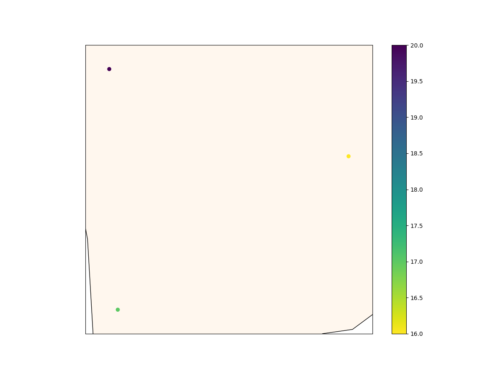
\includegraphics{images/__f.hypotheses.org_wp-content_blogs.dir_4500_files_2018_11_alorese-500x375.png}
\captionsetup{justification=centering}
\caption*{\small \textbf{Figure 1}: Number of forms given in the abridged Alorese dataset, for each
of the three different dialects. The black line is the coastline of the
birdshead peninsula of the island of Alor.}
\end{figure}

Another interesting tool to analyze CLDF wordlists comes in the Python
library accompanying the LexiRumah dataset (Kaiping, Edwards \& Klamer
2019): For creating orthographies for the languages in that dataset, we
needed to know what sounds they use. The
\passthrough{\lstinline!pylexirumah.get\_phonetic\_inventories!} module
goes through the CLDF wordlist and counts the frequency of all segments
that appear, both per-language and overall.

\begin{lstlisting}
$ python -m pylexirumah.get_phonetic_inventories --dataset Alorese-Lects-metadata.json
alk
    a   11
    o   8
    i   8
    e   7
    m   5
    k   4
    n   4
    r   4
    f   3
    p   3
    h   2
    _   2
    g   2
    ŋ   2
    l   1
    lː  1
    ã  1
    u   1
dul
    a   16
    i   6
    e   5
    _   5
    n   5
    t   5
    r   4
    f   3
    ŋ   3
    p   3
    u   3
    g   3
    dʒ  3
    ɔ   3
    h   2
    o   2
    ɛ   2
    m   2
    k   1
    l   1
    h̃  1
    eː  1
alb
    a   18
    n   8
    i   7
    g   6
    _   5
    r   5
    ə   5
    m   5
    f   4
    e   4
    ŋ   4
    ɔ   4
    k   3
    p   3
    o   3
    h   2
    u   2
    l   2
    t   2
    dʒ  1
    ɛ   1
    ;   1
    ã  1
Summa
    a   45
    i   21
    n   17
    e   16
    o   13
    r   13
    _   12
    m   12
    g   11
    f   10
    ŋ   9
    p   9
    k   8
    ɔ   7
    t   7
    h   6
    u   6
    ə   5
    dʒ  4
    l   4
    ɛ   3
    ã  2
    lː  1
    ;   1
    eː  1
    h̃  1
\end{lstlisting}

This again shows that the data is not entirely clean --
\lstinline!;! and \lstinline!h̃! are both
unexpected as phonetic segments.

Any other CLDF Wordlist tool you might come along should also work with
this dataset. For example, have a look at
\href{https://github.com/lexibank/pylexibank}{pylexibank} (Forkel 2018),
the python package for working with the Wordlists in the
\href{https://glottobank.org/\#lexibank}{LexiBank} project. The list of
useful tools also includes the BEASTling tool for generating
phylogenetic inference driver files, which we will work with in the next
step.

\subsection*{References}

\nopagebreak\hangindent=0.7cm {\small Forkel, Robert. 2018. \emph{pylexibank} . Python. lexibank.
\url{https://github.com/lexibank/pylexibank} (19 January, 2019). }

\nopagebreak\hangindent=0.7cm {\small Forkel, Robert, Sebastian Bank, Gereon A. Kaiping, Christoph Rzymski \&
Simon J. Greenhill. 2018. \emph{pycldf} . Python. Cross-Linguistic Data
Formats. \url{https://github.com/cldf/pycldf} (19 January, 2019). }

\nopagebreak\hangindent=0.7cm {\small Forkel, Robert, Christoph Rzymski, Gereon A. Kaiping \& Mattis List.
2019. \emph{The CLDF Cookbook} . Jupyter Notebook. Cross-Linguistic Data
Formats. \url{https://github.com/cldf/cookbook} (19 January, 2019). }

\nopagebreak\hangindent=0.7cm {\small Kaiping, Gereon A., Owen Edwards \& Marian Klamer. 2019. \emph{LexiRumah
2.0.0} . Zenodo. doi: \href{https://doi.org/10.5281/zenodo.2540954.}{10.5281/zenodo.2540954.}
\url{https://zenodo.org/record/2540954\#.XENYWaHrC00} (19 January,
2019). }

\nopagebreak\hangindent=0.7cm {\small List, Johann-Mattis, Michael Cysouw \& Robert Forkel (eds.).
2016. \emph{Concepticon} . Jena: Max Planck Institute for the Science of
Human History. doi:
\href{https://doi.org/10.5281/zenodo.51259.}{10.5281/zenodo.51259.}
\url{http://concepticon.clld.org/}. }


\vskip 2em
\framebox{\tabular{p{0.95\textwidth}}\textbf{Cite this article as}:
Gereon A. Kaiping,
\enquote{From Fieldwork to
Trees 3: CLDF recipes,}
in \emph{Computer-Assisted Language Comparison in Practice},
21/01/2019, \url{https://calc.hypotheses.org/867}.\endtabular}


\newpage
\section*{A Primer on Automatic Inference of Sound Correspondence
Patterns (1): Introduction}
\phantomsection\addcontentsline{toc}{section}{A Primer on Automatic Inference of Sound Correspondence
Patterns (1): Introduction (Johann-Mattis List)}

Johann-Mattis List (30/01/2019)

\emph{Categories}: Primer

\emph{Tags}: cognate detection, correspondence patterns, phonetic
alignment, tutorial

\begin{center}\rule{0.5\linewidth}{1pt}\end{center}

After about three years of work on the matter, I have managed (with help
of many colleagues who helped in testing) to develop a first approach
for the \emph{automatic inference of sound correspondence patterns} ,
which will soon be published with Computational Linguistics
\href{http://bibliography.lingpy.org?key=List2019a}{(List 2019)} . The
key task which this algorithm solves is to take aligned data as input
and to compute explicit \emph{sound correspondence patterns} from the
alignments.

Correspondence patterns are hereby understood as recurring alignment
sites (i.e., columns per alignment) in a given dataset. In contrast to
\emph{regular sound correspondences} (or \emph{systematic sound
correspondences} , as
\href{http://bibliography.lingpy.org?key=Trask2000}{Trask 2000} calls
them), a correspondence pattern is a statement of sound correspondences
across multiple languages, while regular sound correspondences are
usually discussed for two languages only, at least in automatic (see
\href{http://bibliography.lingpy.org?key=Kondrak2002a}{Kondrak 2002} )
and formal approaches (see e.g.,
\href{http://bibliography.lingpy.org?key=Hoenigswald1960}{Hoenigswald
1960} ).

The result of an automatic correspondence pattern analysis can be
thought of as some kind of a table, in which languages are placed in the
columns, and correspondence patterns are placed in rows, with each cell
indicating for each individual correspondence pattern, which reflex
sound a given language shows for this pattern.

As an example, consider the following table, which shows four varieties
of the Tableaux Phonétiques des Patois Suisses Romands (
\href{http://bibliography.lingpy.org?key=Gauchat1925}{Gauchat et al.
1925} ), which were included as test set for the alignment algorithm
presented in my thesis (
\href{http://bibliography.lingpy.org?key=List2014d}{List 2014} ).

\begin{longtable}[]{@{}llllll@{}}
\toprule
Pattern & Frequency & Champéry & Lourtier & Plagne &
Courtedoux\tabularnewline
\midrule
\endhead
` r   & 21 & r  & r  & r  & r  \tabularnewline
`-(1) & 8  & -- & -- & ə  & -- \tabularnewline
` t   & 8  & t  & t  & t  & t  \tabularnewline
` m   & 8  & m  & m  & m  & m  \tabularnewline
` f   & 8  & f  & f  & f  & f  \tabularnewline
` p   & 7  & p  & p  & p  & p  \tabularnewline
`-(2) & 4  & -- & -- & -- & ə  \tabularnewline
` s   & 4  & s  & ʃ  & s  & s  \tabularnewline
` k   & 3  & k  & k  & k  & tʲ \tabularnewline
\bottomrule
\end{longtable}

The table provides some ecclectic information (and I could easily
provide more), namely some \enquote{identifier} for the pattern (which I
created in an ad-hoc manner here), the frequency of attested alignment
sites, where the pattern occurs, and the concrete reflexes in the four
varieties.

While most of the patterns look boring, showing the same reflex in all
varieties (which should not be surprising, given that we're dealing with
dialect data here), some show some degree of variation, such as the two
patterns which I label as \passthrough{\lstinline!*!}-(1) and
\passthrough{\lstinline!*!}-(2), respectively, or the pattern
\passthrough{\lstinline!*!} s and \passthrough{\lstinline!*!} ku. The
first two patterns illustrate different degrees of metathesis across the
varieties, as they surface in words like \enquote{du poivre}, where
prototypical reflexes would be Champéry \passthrough{\lstinline![!}
paːvro \passthrough{\lstinline!]!} as opposed to Plagne
\passthrough{\lstinline![!} paːvər \passthrough{\lstinline!]!} for the
first, and Champéry \passthrough{\lstinline![!} pɛrdy
\passthrough{\lstinline!]!} as opposed to Courtedoux
\passthrough{\lstinline![!} prədʒy \passthrough{\lstinline!]!} . The
\passthrough{\lstinline!*!} s pattern illustrates the pronunciation of
original \passthrough{\lstinline![!} s \passthrough{\lstinline!]!} as
\passthrough{\lstinline![!} ʃ \passthrough{\lstinline!]!} in initials in
Lourtrier, and the third pattern illustrates a specific palatalization
process of velars in Courtedoux.

What is interesting and important about these data is how useful they
are for additional tasks in historical linguistics. Correspondence
patterns can, for example, be used to \emph{predict} the pronunciation
of missing reflexes in a given dataset (as I show in my forthcoming
paper, \href{http://bibliography.lingpy.org?key=List2019a}{List 2019} ),
they can also be used to reconstruct a given ancestor form
semi-automatically, given that all alignment sites which are assigned to
the same correspondence pattern directly reflect the same common
ancestor sound, and they can be used to investigate conditioning
context, given that patterns that look very similar but differ regarding
the reflexes of a few varieties often derive from the same proto-sound
whose change was then modified in specific environments.

While correspondence patterns can be investigated manually, and people
have been doing this in the past, the new computer-assisted methods
which we have developed so far greatly facilitate the systematic
investigation of correspondence patterns in historical linguistics. The
only problem is that --- in order to successfully carry out an automatic
search for sound correspondence patterns, the data needs to be provided
in a very good state, with a very high level of consistency and
annotation.

In the following couple of weeks, I want to provide examples for
different datasets, illustrating how these can be analyzed with help of
the tools for automatic correspondence pattern detection, which have
been developed in the past. In this context, I plan to select different
datasets and show how they have to be prepared in order to properly
analyze them. The posts will be accompanied by supplementary data and
code, so that interested users can directly apply and test the examples
discussed.

\subsection*{References}

\nopagebreak\hangindent=0.7cm {\small Gauchat, Louis and Jeanjaquet, Jules and Tappolet, Ernest (1925):
Tableaux phonétiques des patois suisses romands. Relevés comparatifs
d'environ 500 mots dans 62 patois-types. Publiés avec introduction,
notes, carte et répertoires . Neuchâtel:Attinger. }

\nopagebreak\hangindent=0.7cm {\small Hoenigswald, Henry M. (1960): Phonetic similarity in internal
reconstruction. \emph{Language} 36.2. 191-192. }

\nopagebreak\hangindent=0.7cm {\small Kondrak, Grzegorz (2002): Determining Recurrent Sound
Correspondences by Inducing Translation Models. In: Nineteenth
International Conference on Computational Linguistics (COLING 2002).
488-494. }

\nopagebreak\hangindent=0.7cm {\small List, Johann-Mattis (2014): Sequence comparison in historical
linguistics. Düsseldorf:Düsseldorf University Press. }

\nopagebreak\hangindent=0.7cm {\small List, Johann-Mattis (forthcoming): Automatic inference of sound
correspondence patterns across multiple languages. \emph{Computational
Linguistics} ?? 1-24. }

\nopagebreak\hangindent=0.7cm {\small Trask, Robert L. (2000): The dictionary of historical and
comparative linguistics . Edinburgh:Edinburgh University Press. }

\vskip 2em
\framebox{\tabular{p{0.95\textwidth}}\textbf{Cite this article as}:
Johann-Mattis List,
\enquote{A Primer on
Automatic Inference of Sound Correspondence Patterns (1): Introduction,}
in \emph{Computer-Assisted Language Comparison in Practice},
30/01/2019, \url{https://calc.hypotheses.org/1802}.\endtabular}

\newpage
\section*{A Primer on Automatic Inference of Sound Correspondence
Patterns (2): Initial Experiments with Alignments from the Tableaux
Phonétiques des Patois Suisses Romands}
\phantomsection\addcontentsline{toc}{section}{A Primer on Automatic Inference of Sound Correspondence
Patterns (2): Initial Experiments with Alignments from the Tableaux
Phonétiques des Patois Suisses Romands (Johann-Mattis List)}

Johann-Mattis List (27/02/2019)

\emph{Categories}: Analysis, Primer

\emph{Tags}: Benchmark Database of Phonetic Alignments, correspondence
patterns, EDICTOR, LingPy, Python, Tableaux Phonétiques des Patois
Suisses Romands

\begin{center}\rule{0.5\linewidth}{1pt}\end{center}

Following up on my announcement to present in more detail how the
algorithms for automatic correspondence pattern detection can be
applied, this post introduces the preliminary preparations needed to run
a first experiment with aligned data. In order to avoid that we have to
align a dataset completely from scratch, we make use of already aligned
data from the Tableaux Phonétiques des Patois Suisses Romands by
\href{http://bibliography.lingpy.org?key=Gauchat1925}{Gauchat et
al.~(1925)}, which were originally aligned for the study in
\href{http://bibliography.lingpy.org?key=List2014d}{List (2014)} and
later published as part of the
\href{http://alignments.lingpy.org}{Benchmark Database of Phonetic
Alignments} \href{http://bibliography.lingpy.org?key=List2014e}{(List
and Prokić 2014)} . In this post, I will introduce how we can harvest
the alignments from this dataset with help of
\href{http://lingpy.org}{LingPy} , and later analyze them with help of
the sound correspondence pattern algorithms.

The Tableaux Phonétiques des Patois Suisses Romands (Gauchat et al.
1925) is a large collection of dialect data on French dialects spoken in
Switzerland. Originally collected by Gauchat and colleagues, it was
digitized in a project by Hans Geisler (Heinrich Heine Universität
Düsseldorf) but could by then not be published officially due to
copyright restrictions. Fortunately, however, I could use parts of the
data for my dissertation (List 2014), where I aligned 76 of the charts
for as many as 62 dialect points. While the data in its form used by
then can still be interactively searched from the website offering all
\href{https://sequencecomparison.github.io}{supplementary material
accompanying my dissertation} , I figured later that it would be better
to share it officially as part of a larger benchmark database of
phonetic alignments, which I published together with Jelena Prokić, who
contributed alignments for Bulgarian dialects to that sample (List and
Prokić 2014). This \href{http://alignments.lingpy.org}{Benchmark
Database of Phonetic Alignments} (BDPA) offers a potentially more
convenient way of browsing and inspecting alignment data, although the
data is not necessarily offered in a convenient form to reuse.

As of now, the original alignment data underlying the BDPA has also been
submitted to \href{https://zenodo.org/record/11880}{Zenodo} , from where
it can still be downloaded. The data on the Zenodo repository is of a
very simple structure, containing a bunch of zip-folders for each of the
different datasets from which we harvested the alignments, along with
two redundant master-folders, containing all 750 multiple sequence
alignments. Each of the folders contains two sub-folders, one called
\passthrough{\lstinline!msa!} , containing the multiple alignments in
the so-called \passthrough{\lstinline!msa-format!} , which can be
readily imported and processed by LingPy, as well as a
\passthrough{\lstinline!psa!}-folder, containing all corresponding
pairwise phonetic alignments (i.e., pairwise alignments automatically
derived from the multiple alignments by extracting all possible pairs).

The \passthrough{\lstinline!msa!}-format is basically outdated, and we
don't use it anymore, although LingPy still parses it. For testing
purposes, this is quite useful, although we now usually tend to use
alignments exclusively in wordlists, where we have more consistent ways
of handling the data, and also doing more interesting analyses. The
\passthrough{\lstinline!msa!}-format is described in detail on the
\href{http://lingpy.org/tutorial/formats.html\#multiple-alignments-msq-and-msa}{LingPy
website}, so I will spare the readers and myself a closer description
here. What is important to know is that we want to convert those files
corresponding to the TPPSR in the BDPA, asprovided in
\passthrough{\lstinline!msa!}-format on Zenodo to the \enquote{normal}
\emph{wordlist-format} , as it is used by the LingPy package (see
\href{http://bibliography.lingpy.org?key=List2018d}{List et al. 2018}
for a closer description) and also required in order to compute
correspondence patterns with help of
\href{https://github.com/lingpy/lingrex}{LingRex} and the correspondence
pattern recognition algorithm (
\href{http://bibliography.lingpy.org?key=List2019a}{List 2019} ).

Assuming that you have downloaded the data from Zenodo and unpacked the
\passthrough{\lstinline!multiple.zip!} folder, placing the
\passthrough{\lstinline!msa!}-folder in your current working directory
(or \passthrough{\lstinline!cd!}-ing into it), we can now get started to
convert the data. Our goal is to select some 15 representative dialects
from the data, extract their alignments, and store them in the
wordlist-format, so that we can later analyze the correspondence
patterns in the data. We thus start by setting up our Python script in
which we import the packages required:

\begin{lstlisting}
from lingpy import *
from glob import glob
import re
import tqdm
from lingpy.align.sca import normalize_alignment
\end{lstlisting}

We use \passthrough{\lstinline!glob!} to retrieve the paths of the
files, and \passthrough{\lstinline!tqdm!} to have a status bar that
informs us about the process. We further need the
\passthrough{\lstinline!re!} module to retrieve some information about
the data, \passthrough{\lstinline!lingpy!} in general, and the
\passthrough{\lstinline!normalize\_alignment!} function in specific.
This latter function will delete all those columns from an alignment,
which consist only of gaps. This can happen when taking only a small
selection of language varieties from a larger selection of aligned
words.

We can now retrieve all files with help of
\passthrough{\lstinline!glob!} .

\begin{lstlisting}
files = glob('msa/*.msa')
\end{lstlisting}

To make sure that we find the varieties we want, I made a manual
pre-selection, which we represent as a Python dictionary:

\begin{lstlisting}
selection = {'Boudry': '46',
 'Cerneux-Péquignot': '53',
 'Champéry': '18',
 'Courtedoux': '62',
 'Courtepin': '41',
 'Côte-aux-Fées': '50',
 'Dompierre': '42',
 'Evolène': '30',
 'Grimentz': '31',
 'Hermance': '36',
 'Lourtier': '22',
 'L’Auberson': '3',
 'Ormont-Dessus': '15',
 'Plagne': '56',
 }
\end{lstlisting}

We also represent our wordlist as a Python dictionary, where the
\passthrough{\lstinline!0!}-key represents the column header.\\
~\\

\begin{lstlisting}
D = {0: [
    'doculect',
    'language_id',
    'concept',
    'latin',
    'french',
    'form',
    'tokens',
    'alignment',
    'cogid'
    ]}
\end{lstlisting}

As we want to fill the wordlist with identifiers for the words
themselves and for cognates consecutively, we set them now as variables.

\begin{lstlisting}
idx, cogid = 1, 1
\end{lstlisting}

We also define a very lazy converter, since we want to replace all
underscores in the alignments by a \passthrough{\lstinline!+!} symbol,
which is now the standard marker for morpheme boundaries, which we
decided for during the last year (but older versions have still the
underscore \passthrough{\lstinline!\_!} as a marker for word
boundaries).

\begin{lstlisting}
converter = {
        '_': '+'
        }
\end{lstlisting}

We can now start by looping over all files and extracting the relevant
data. In this loop, we open each of the
\passthrough{\lstinline!msa!}-files with help of LingPy, and assess it's
\passthrough{\lstinline!dataset!} property. If the dataset is
\passthrough{\lstinline!French!} , we keep the file and try to process
it further. We use a regular expression to parse the HTML-like coding of
the so-called \passthrough{\lstinline!sequence identifier!} of the
alignment, which is the counterpart of the aligned word forms in French
and its projected ancestral form in Latin. Since the
\passthrough{\lstinline!msa!} format does not specify how the dataset or
the sequence identifier should be structured, the formats are pretty
free, and by then, I used HTML-like tags for convenience (1).

Once we have extracted the dataset, made sure it is
\passthrough{\lstinline!French!} , and also extracted the Latin and the
French word form, we can extract the aligned data from the
\passthrough{\lstinline!MSA!}-object, stored in the variable
\passthrough{\lstinline!msa!} . Here, we iterate over its properties
\passthrough{\lstinline!msa.taxa!} and
\passthrough{\lstinline!msa.alignment!} and check if the name of the
variety also occurs in our dictionary of pre-selected varieties. If this
is the case, we retrieve the unaligned but segmented form (called
\passthrough{\lstinline!tokens!} ) by stripping off all dashes from the
alignment, and we also retrieve the raw, unsegmented
\passthrough{\lstinline!form!} by even deleting the spaces that would
otherwise indicate the boundaries between the sound segments.

We can now add all data to our wordlist (or our dictionary, 3), but we
should not forget to incremend the index for the word identifier (
\passthrough{\lstinline!idx!} ) and the cognate set identifier (
\passthrough{\lstinline!cogid!} ).

\begin{lstlisting}
for f in tqdm.tqdm(files):
    # (1: initiate MSA object)
    msa = MSA(f)
    if msa.dataset == 'French':
        french, latin = re.findall(
                r'\*(.*?)\*',
                msa.seq_id
                )
        # (2: extract alignments)
        for taxon, alm in zip(msa.taxa,
                msa.alignment):
            taxon_id = selection.get(taxon, '')
            if taxon_id:
                tokens = [converter.get(
                    x,
                    x
                    ) for x in alm if x != '-']
                form = ''.join(tokens)
                # (3: add data to wordlist)
                D[idx] = [
                        taxon,
                        taxon_id,
                        french,
                        latin,
                        french,
                        form,
                        tokens,
                        alm,
                        cogid
                        ]
                idx += 1
        cogid += 1
\end{lstlisting}

Now that we have assembled the data readily, we can load it with help of
LingPy's \passthrough{\lstinline!Alignments!} class, which we call by
passing the dictionary with \passthrough{\lstinline!cogid!} as the
keyword for the \emph{reference} ( \passthrough{\lstinline!ref!} ),
which we use to construct our alignments.

\begin{lstlisting}
alms = Alignments(D, ref='cogid')
\end{lstlisting}

We need to do this in order to make sure that all alignments are
\enquote{normalized}, i.e., they should not contain empty columns. We do
this by iterating over all alignments in the
\passthrough{\lstinline!Alignments!} object, which we can access as a
dictionary, in which the key is the cognate identifier, and the value is
a dictionary identical with the data needed to construct an
\passthrough{\lstinline!MSA!} object. The normalization is now
straightforward, and we re-write all individual alignments attached to
individual word forms to make sure this is readily stored.

\begin{lstlisting}
for cogid, msa in alms.msa['cogid'].items():
    for idx, alm in zip(
            msa['ID'],
            normalize_alignment(
                msa['alignment']
                )
            ):
        alms[idx, 'alignment'] = alm
\end{lstlisting}

We can now write the data to file. By passing the
\passthrough{\lstinline!prettify!} keyword and setting it to
\passthrough{\lstinline!False!} , we make sure that the data will be
written to plain TSV format.

\begin{lstlisting}
alms.output(
        'tsv',
        filename='tppsr-bdpa',
        prettify=False
        )
\end{lstlisting}

How we can use this file to calculate correspondence patterns with help
of the correspondence pattern recognition algorithm described in List
(2019) is something I will describe in more detail in a follow-up post.
But what we can do already with the data by now is loading it into
\href{http://edictor.digling.org}{EDICTOR} (
\href{http://bibliography.lingpy.org?key=List2017d}{List 2017} ), and
use the built-in tool for correspondence pattern analyses. This tool is
less accurate than the Python implementation in the LingRex package,
since it is written in plain JavaScript. All it does is that it tries to
sort the sound correspondences in a rather smart way, using JavaScripts
rather convenient ways to sort arrays. This works --- at least to some
degree--- surprisingly well, as you can see yourself, when opening the
EDICTOR at \url{http://edictor.digling.org} and then either dragging the
file \passthrough{\lstinline!tppsr-bdpa.tsv!} to the BROWSE button or
selecting it by clicking on this button. You then click on ANALYZE in
the menu, and select CORRESPONDENCE PATTERNS from there. Select
\enquote{full cognates}, as we are not dealing with partial cognates
here, and press OK.

\begin{figure}[htb]
\centering
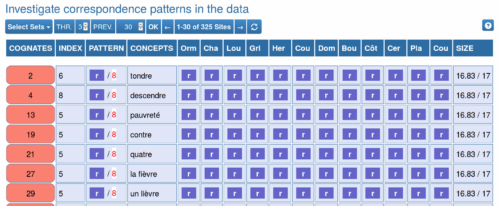
\includegraphics[width=\textwidth]{images/__f.hypotheses.org_wp-content_blogs.dir_4500_files_2019_02_edictor1-500x206.png}
\captionsetup{justification=centering}
\caption*{\small \textbf{Figure 1}: Correspondence pattern display in EDICTOR.}
\end{figure}

What you will see is a collection of all your correspondence patterns
which EDICTOR's simple method extracts from the alignments.The
arrangement is by language variety in the columns, and by cognate set
(or alignemnt) in each row. By clicking on a given value, EDICTOR will
show you the full word for that entry.

\begin{figure}[htb]
\centering
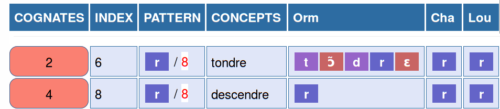
\includegraphics[width=\textwidth]{images/__f.hypotheses.org_wp-content_blogs.dir_4500_files_2019_02_edictor2-500x109.png}
\captionsetup{justification=centering}
\caption*{\small \textbf{Figure 2}: Viewing original words for a given correspondence pattern.}
\end{figure}


Clicking on the cognate ID on the very left, it will show you the
alignment.

\begin{figure}[htb]
\centering
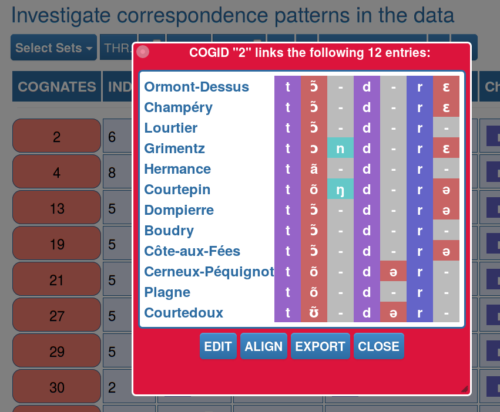
\includegraphics[width=\textwidth]{images/__f.hypotheses.org_wp-content_blogs.dir_4500_files_2019_02_edictor3-500x412.png}
\captionsetup{justification=centering}
\caption*{\small \textbf{Figure 2}: Alignment popups in EDICTOR's correspondence pattern viewer.}
\end{figure}

It would take too long to describe all possibilities for searching here,
so I recommend those interested in exploring this further, to simply
download the dataset, prepared with the script described here from the
\href{https://gist.github.com/LinguList/994317214fbdc78460feb551b113b05f}{Github.Gist}
accompanying this tutorial, and see yourself what can be done. If you
have ideas on how the tool could be enhanced, I would furthermore be
happy about any kind of feedback or questions or suggestions, which you
shoudl ideally share via our project page with
\href{https://github.com/digling/edictor}{GitHub/digling/edictor} .

\subsection*{References}

\nopagebreak\hangindent=0.7cm {\small Gauchat, Louis and Jeanjaquet, Jules and Tappolet, Ernest (1925):
Tableaux phonétiques des patois suisses romands. Relevés comparatifs
d'environ 500 mots dans 62 patois-types. Publiés avec introduction,
notes, carte et répertoires . Neuchâtel:Attinger. }

\nopagebreak\hangindent=0.7cm {\small List, Johann-Mattis (2014): Sequence comparison in historical
linguistics. Düsseldorf:Düsseldorf University Press. }

\nopagebreak\hangindent=0.7cm {\small List, J.-M. and Prokić, J. (2014): A benchmark database of phonetic
alignments in historical linguistics and dialectology. In: Proceedings
of the Ninth International Conference on Language Resources and
Evaluation. 288-294. }

\nopagebreak\hangindent=0.7cm {\small List, Johann-Mattis (2017): A web-based interactive tool for
creating, inspecting, editing, and publishing etymological datasets. In:
Proceedings of the 15th Conference of the European Chapter of the
Association for Computational Linguistics. System Demonstrations.
9-12. }

\nopagebreak\hangindent=0.7cm {\small List, Johann-Mattis and Walworth, Mary and Greenhill, Simon J. and
Tresoldi, Tiago and Forkel, Robert (2018): Sequence comparison in
computational historical linguistics. \emph{Journal of Language
Evolution} 3.2. 130--144. }

\nopagebreak\hangindent=0.7cm {\small List, Johann-Mattis (2019): Automatic inference of sound
correspondence patterns across multiple languages. \emph{Computational
Linguistics} 1.45. 1-24. }

\vskip 2em
\framebox{\tabular{p{0.95\textwidth}}\textbf{Cite this article as}:
Johann-Mattis List,
\enquote{A Primer on
Automatic Inference of Sound Correspondence Patterns (2): Initial
Experiments with Alignments from the Tableaux Phonétiques des Patois
Suisses Romands,}
in \emph{Computer-Assisted Language Comparison in Practice},
27/02/2019, \url{https://calc.hypotheses.org/1807}.\endtabular}

\newpage
\section*{A Primer on Automatic Inference of Sound Correspondence
Patterns (3): Extended Experiments with Alignments from the Tableaux
Phonétiques des Patois Suisses Romands}
\phantomsection\addcontentsline{toc}{section}{A Primer on Automatic Inference of Sound Correspondence
Patterns (3): Extended Experiments with Alignments from the Tableaux
Phonétiques des Patois Suisses Romands (Johann-Mattis List)}

Johann-Mattis List (27/03/2019)

\emph{Categories}: Code, Primer

\emph{Tags}: correspondence patterns, introduction, Python, TPPSR

\begin{center}\rule{0.5\linewidth}{1pt}\end{center}

Having illustrated how a quick correspondence pattern analysis can be
done with help of readily formatted data and the
\href{http://edictor.digling.org}{EDICTOR} tool alone, it is now time to
show how we can use the
\href{https://github.com/lingpy/lingrex}{LingRex} package in order to
carry out a full-fledged correspondence pattern analysis. While EDICTOR
uses a simple algorithm that is based on sorting the patterns, the
Python algorithm for correspondence pattern detection, which is
described in detail in
\href{http://bibliography.lingpy.org?key=List2019a}{List (2019)} , uses
a greedy approach inspired by the Welsh-Powell algorithm for graph
coloring ( \href{http://bibliography.lingpy.org?key=Welsh1967}{Welsh and
Powell 1967} ), in order to cluster all alignment sites in the data into
clusters which are compatible with each other.

In the following, I will demonstrate how the LingRex package, which I
plan to include into \href{http://lingpy.org}{LingPy} in the future,
after sufficient tests have been written, can be used to apply the
correspondence pattern detection algorithm, and how the results can ---
again --- be investigated with help of EDICTOR. In order to get started,
you should make sure to install the package with its dependencies. In
order to do so, the easiest way is to download the package from GitHub
or to clone it with GIT, and to install the depencencies with help of
PIP.

\begin{lstlisting}
$ git clone https://github.com/lingpy/lingrex.git
$ cd lingrex
$ pip install -r pip-requirements.txt
$ python setup.py develop
\end{lstlisting}

As data for testing, we will use the same dataset of 70 alignments taken
from the \emph{Tableaux Phonétiques des Patois Suisses Romands} (
\href{http://bibliography.lingpy.org?key=Gauchat1925}{Gauchat et
al.~1925} ), which were included as alignments in the \emph{Benchmark
Database for Phonetic Alignments} (http://alignments.lingpy.org,
\href{http://bibliography.lingpy.org?key=List2014e}{List and Prokić
2014} ). Now, that the data has already been prepared as a wordlist that
can be accessed by LingPy and EDICTOR, we can directly access it from
Python. Since LingRex uses LingPy's datastructures, it expects the same
data as input. In fact, the major class that we will use to carry out
the correspondence pattern detection is an extension of LingPy's
\passthrough{\lstinline!Alignments!} class which can be used to handle
alignments in wordlists. That means, that all the functions that are
available as part of the \passthrough{\lstinline!Alignments!} class in
LingPy are also available as part of the \passthrough{\lstinline!CoPaR!}
class in LingRex. We thus start by loading the data.

\begin{lstlisting}
from lingrex.copar import CoPaR
cop = CoPaR(
    'tppsr-bdpa.tsv',
    ref='cogid',
    segments='tokens'
)
print('{0} / {1} / {2}'.format(
    cop.height,
    cop.width,
    len(cop)
)
\end{lstlisting}

Now that we have imported the data, we need to add prosodic information
to all sequences. This information serves as some kind of an initial
clustering of the data, based on the prosodic environment of a given
alignment site. In its simplest form, we treat all sites alike. But
since we know, for example, that our alignments never place a vowel and
a consonants into the same column, we can already use that information
to make the task a little bit easier for the algorithm. This can be done
by adding, what is called \passthrough{\lstinline!structure!} in the
LingRex package.

\begin{lstlisting}
cop.add_structure(model='cv', structure='structure')
\end{lstlisting}

This method will add another column to our data, in which each sound
sequence is characterized by a string that indicates if the segment is a
vowel or a consonant. The result of this can be seen when looking at the
first ten entries of our wordlist, as shown in the table below.

\begin{longtable}[]{@{}llll@{}}
\toprule
ID & DOCULECT & TOKENS & STRUCTURE\tabularnewline
\midrule
\endhead
1 & Ormont-Dessus & ʃ e & C V\tabularnewline
2 & Champéry & ʃ i & C V\tabularnewline
3 & Lourtier & ʃ e & C V\tabularnewline
4 & Grimentz & ʃ aː & C V\tabularnewline
5 & Hermance & s e & C V\tabularnewline
6 & Courtepin & ʃ eː & C V\tabularnewline
7 & Dompierre & s e & C V\tabularnewline
8 & Boudry & s aː & C V\tabularnewline
9 & Côte-aux-Fées & s a & C V\tabularnewline
10 & Cerneux-Péquignot & s aː v u & C V C V\tabularnewline
\bottomrule
\end{longtable}

Now that we have added the \passthrough{\lstinline!STRUCTURE!} to our
data, we can start with the real analysis. We start by retrieving the
alignment sites with all relevant information, restricting the sites we
consider to those which have at least two reflexes (indicated by the
\passthrough{\lstinline!minrefs!} keyword).

\begin{lstlisting}
cop.get_sites(minrefs=2, structure='structure')
\end{lstlisting}

This method will add a new attribute to our
\passthrough{\lstinline!CoPaR!} object, called
\passthrough{\lstinline!sites!} . These sites are organized as a
dictionary, with tuples of the cognate identifier and the position in
the alignment as a key, and the structure (if it is consonant or vowel,
in our case) along with the concrete alignment site as a value. If a
site contains missing entries, this is by default represented with help
of the symbol \passthrough{\lstinline!Ø!} , which we use to denote
missing data (in contrast to \passthrough{\lstinline!-!} denoting a gap
in an alignment. The following table illustrates this for the cognate
sets 31 and 63 in the data, which contain reflexes for the concepts
\emph{le chasseur} and \emph{la hache} , with the latter being only
reflected in 8 out of 12 varieties in our dataset. The alignment site
column shows the reflex for each variety in alphabetical order by the
variety name.

\begin{longtable}[]{@{}llll@{}}
\toprule
COGID & POSITION & STRUCTURE & ALIGNMENT SITE\tabularnewline
\midrule
\endhead
31 & 0 & C & \enquote{ts}, \enquote{tʃ}, \enquote{ts}, \enquote{tʃ},
\enquote{ts}, \enquote{ts}, \enquote{ts}, \enquote{ts}, \enquote{θ},
\enquote{ts}, \enquote{ts}, \enquote{tʃ}\tabularnewline
31 & 1 & V & \enquote{a}, \enquote{ɛ}, \enquote{a}, \enquote{-},
\enquote{a}, \enquote{a}, \enquote{a}, \enquote{a}, \enquote{ɛ},
\enquote{a}, \enquote{a}, \enquote{-}\tabularnewline
31 & 2 & C & \enquote{s}, \enquote{s}, \enquote{ç}, \enquote{s},
\enquote{ç}, \enquote{ʃ}, \enquote{ç}, \enquote{s}, \enquote{f},
\enquote{ç}, \enquote{-}, \enquote{s}\tabularnewline
31 & 3 & V & \enquote{œː}, \enquote{u}, \enquote{œː}, \enquote{u},
\enquote{aː}, \enquote{œ}, \enquote{aː}, \enquote{ou}, \enquote{œ},
\enquote{ɔː}, \enquote{au}, \enquote{u}\tabularnewline
31 & 4 & C & \enquote{r}, \enquote{-}, \enquote{-}, \enquote{-},
\enquote{-}, \enquote{-}, \enquote{-}, \enquote{-}, \enquote{-},
\enquote{-}, \enquote{-}, \enquote{-}\tabularnewline
63 & 0 & C & \enquote{ts}, \enquote{tʃ}, \enquote{Ø}, \enquote{tʃ},
\enquote{ts}, \enquote{ts}, \enquote{ts}, \enquote{Ø}, \enquote{θ},
\enquote{Ø}, \enquote{Ø}, \enquote{tʃ}\tabularnewline
63 & 1 & V & \enquote{-}, \enquote{ɔ}, \enquote{Ø}, \enquote{ɑ},
\enquote{ɛ}, \enquote{-}, \enquote{ɛ}, \enquote{Ø}, \enquote{õ},
\enquote{Ø}, \enquote{Ø}, \enquote{a}\tabularnewline
63 & 2 & C & \enquote{-}, \enquote{t}, \enquote{Ø}, \enquote{t},
\enquote{t}, \enquote{-}, \enquote{t}, \enquote{Ø}, \enquote{-},
\enquote{Ø}, \enquote{Ø}, \enquote{t}\tabularnewline
63 & 3 & V & \enquote{-}, \enquote{ɛ}, \enquote{Ø}, \enquote{-},
\enquote{a}, \enquote{-}, \enquote{a}, \enquote{Ø}, \enquote{-},
\enquote{Ø}, \enquote{Ø}, \enquote{-}\tabularnewline
\bottomrule
\end{longtable}

Now that we have stored the alignment sites, we can start clustering
them.

\begin{lstlisting}
cop.cluster_sites()
\end{lstlisting}

This analysis will add another property to our
\passthrough{\lstinline!CoPaR!} object, called
\passthrough{\lstinline!clusters!} . This is again a Python dictionary,
consisting of the structure segment and the pattern as a key, and the
alignment sites, represented by cognate identifier and position as
value. If we now check in the data for the alignment sites for cognate
set number 31 and 63, we can see that the initials in both cognate sets
are assigned to the same pattern (as they are compatible), and that the
last site in cognate set 31 is clustered with the last site in cognate
set 50 (not shown here), while the rest of the sites are singletons,
which do not recur anywhere else in the data. That we find a lot of
singletons in the data is not surprising, given that we have a very
limited number of cognate sets.

In order to analyze the clusters further, we can now make a secondary
analysis, during which we compare all patterns that were inferred in
this run with each alignment site a second time, this time assigning
alignment sites to all patterns with which they are \emph{compatible} .
This may result in a fuzzy clustering, as one alignment site could
easily be compatible with two or more patterns, provided it contains
enough missing data.

\begin{lstlisting}
cop.sites_to_pattern()
\end{lstlisting}

The results of this analysis are stored in the attribute
\passthrough{\lstinline!patterns!} of the
\passthrough{\lstinline!CoPaR!} object, and they are again provided in
form of a Python dictionary, with the cognate set and the position as
the key for the alignment site, and the patterns to which the site was
assigned provided in a list as value, with each pattern represented by
its size, its structure, and the pattern itself. In our analysis, only
three sites occur, which could be assigned to more than one pattern. One
of these is the second column of the alignment of cognate set 24
\emph{m'appeler} , reflected in only three varieties. Given the large
number of missing data in this alignment, it is compatible with seven
different patterns in the data, shown below in the table.

\begin{longtable}[]{@{}llllllllllll@{}}
\toprule
Ø & Ø & Ø & Ø & Ø & Ø & Ø & r & r & Ø & r & Ø\tabularnewline
\midrule
\endhead
r & r & r & r & r & r & r & r & r & r & r & r\tabularnewline
\textbf{l} & r & r & r & r & r & r & r & r & r & r & r\tabularnewline
r & r & r & \textbf{--} & r & r & r & r & r & r & r &
\textbf{--}\tabularnewline
r & r & \textbf{rː} & r & r & r & r & r & r & \textbf{ʁ} & r &
r\tabularnewline
\textbf{--} & r & r & Ø & r & r & r & r & r & r & r & Ø\tabularnewline
r & r & \textbf{--} & r & r & r & r & Ø & r & Ø & Ø & r\tabularnewline
Ø & Ø & r & Ø & Ø & Ø & r & r & Ø & \textbf{ʁ} & Ø & Ø\tabularnewline
\bottomrule
\end{longtable}

Since it is difficult to spot the differences between these patterns, I
have marked all those sounds which are different from a normal \emph{r}
with bold font. We can see that the pattern is indeed compatible with
all seven patterns, and that the seven patterns themselves are
incompatible with each other. We can, however, also see that the
differences are minor. There are different possibilities to explain the
differences. They could be due to errors in the data or the alignments,
they could be due to borrowing, due to individual \emph{irregular} sound
changes, or due to some specific phonetic environment that triggered a
certain sound change in the individual varieties. What holds in all
cases needs to be checked qualitatively, by investigating the variety in
detail.

As a final step, we add the patterns to our wordlist, and write both the
patterns and the wordlist to a new file.

\begin{lstlisting}
cop.add_patterns(ref='patterns')
cop.output('tsv', filename='tppsr-copped')
cop.write_patterns('patterns.tsv')
\end{lstlisting}

This will result in two new files, the file
\passthrough{\lstinline!tppsr-copped.tsv!} being a wordlist, which we
can inspect in EDICTOR, and the file
\passthrough{\lstinline!patterns.tsv!} being a spreadsheet that shows
all patterns for each language variety along with the reflexes and the
alignment sites. If you open the file
\passthrough{\lstinline!tppsr-copped.tsv!} now with EDICTOR and inspect
the correspondence patterns, as shown in the
\href{https://calc.hypotheses.org/1807}{previous post} , you will find,
that EDICTOR displays the patterns inferred with the Python algorithm
instead of using its own simple method. In this way, you can
conveniently investigate the results with the interactive EDICTOR
application that facilitates the detailed inspection of correspondence
pattern data.

Instead of investigating the data further, I will end here, and leave it
to interested readers to check the data and the results themselves. A
script to run the analysis along with the data is available in form of a
GitHub Gist, which you can find
\href{https://gist.github.com/LinguList/6bd37f375c9715e3ecda395e23a17fcb}{here}.

\subsection*{References}

\nopagebreak\hangindent=0.7cm {\small Gauchat, Louis and Jeanjaquet, Jules and Tappolet, Ernest (1925):
Tableaux phonétiques des patois suisses romands. Relevés comparatifs
dénviron 500 mots dans 62 patois-types. Publiés avec introduction,
notes, carte et répertoires . Neuchâtel:Attinger. }

\nopagebreak\hangindent=0.7cm {\small List, J.-M. and Prokić, J. (2014): A benchmark database of phonetic
alignments in historical linguistics and dialectology. In: Proceedings
of the Ninth International Conference on Language Resources and
Evaluation. 288-294. }

\nopagebreak\hangindent=0.7cm {\small List, Johann-Mattis (2019): Automatic inference of sound
correspondence patterns across multiple languages. \emph{Computational
Linguistics} 1.45. 137-161. }

\nopagebreak\hangindent=0.7cm {\small Welsh, D. J. A. and Powell, M. B. (1967): An upper bound for the
chromatic number of a graph and its application to timetabling problems.
\emph{The Computer Journal} 10.1. 85-86. }

\vskip 2em
\framebox{\tabular{p{0.95\textwidth}}\textbf{Cite this article as}:
Johann-Mattis List,
\enquote{A Primer on
Automatic Inference of Sound Correspondence Patterns (3): Extended
Experiments with Alignments from the Tableaux Phonétiques des Patois
Suisses Romands,}
in \emph{Computer-Assisted Language Comparison in Practice},
27/03/2019, \url{https://calc.hypotheses.org/1823}.\endtabular}

\newpage
\section*{Using pyconcepticon to map concept lists}
\phantomsection\addcontentsline{toc}{section}{Using pyconcepticon to map concept lists (Tiago Tresoldi)}

Tiago Tresoldi (01/04/2019)

\emph{Categories}: Analysis, Annotation

\emph{Tags}:

\begin{center}\rule{0.5\linewidth}{1pt}\end{center}

A major problem for data reuse in computer-assisted historical
linguistics, especially when employing data collected with no
computational workflows in mind, is linking datasets in terms of the
meanings of the words (or, technically, \enquote{forms}) they carry.
Just as linking languages across different datasets is not as
straightforward as one might naively assume, demanding a complex
reference catalog such as \href{https://glottolog.org/}{Glottolog} ,
linking the concepts used in a wordlist (a \enquote{concept list}) to
our \href{https://concepticon.clld.org/}{Concepticon} project might well
be the most intensive task in preparing a dataset for cross-linguistic
studies.

We could discuss the more theoretical issues at hand, ranging from
pragmatic lexicographic decisions to deep philosophical disputations on
hermeneutics --- even though it is always worth remembering, Concepticon
is \emph{not} an ontology, but a catalog for linking concept lists.
However, for the time being, let's take a hard-headed view and look at
the practical issues at play. Common issues are: - Plain errors in the
glosses, especially when OCR or typing from published sources is
involved, such as in a recent concept list where I had a typo
\passthrough{\lstinline!barl!} for \passthrough{\lstinline!bark!}
(readers will note how \enquote{L} and \enquote{K} are next to each
other in the most common keyboard layouts).- Problems with homonyms
where the meaning is not specified, such as in
\passthrough{\lstinline!bark!} itself (which could be either a noun, the
\enquote{skin} of a tree, or a verb, \enquote{to bark}) or in the
recurring examples of \passthrough{\lstinline!fly!} (either the insect
or the verb meaning \enquote{to move in the air}) and of
\passthrough{\lstinline!dull!} (either as opposed to \enquote{sharp} or
to \enquote{smart}).- Problems with synonyms, such as in the case of a
word being annotated as \passthrough{\lstinline!eggplant!} in one
concept list but as AUBERGINE in Concepticon.- Glosses given in a
language other than English, and perhaps one you are not entirely
familiar with, or sometimes in multiple languages (like Chinese
\emph{and} English) where the difference in semantics might be more of a
hindrance than a help.

These problems alone would be enough to make concept mapping tedious,
but most people involved in Concepticon would be happy if they were the
only ones. Other common issues can lead almost to frustration are: - The
same dataset using slightly similar (and sometimes visually alike)
glosses for the same concept, such as \passthrough{\lstinline!dog!} and
\passthrough{\lstinline!dog!} (note the trailing whitespace in the
second one).- Just like when reporting forms, authors including all kind
of notes
in their glosses, some useful for the mapping (like
\passthrough{\lstinline!fly (noun)!} ), some
less so (such as \passthrough{\lstinline!poor (dubious)!} ) some which
would better be in a \enquote{Comments} column (like
\passthrough{\lstinline!happy [given by only one speaker]!} ).- People
never shy on coming up with different ways to annotate
additional information, such as part-of-speech, hardly in a consistent
way. Using the flying insect as a common denominator, our collection
already includes specimens such as \passthrough{\lstinline!fly (noun)!}
, \passthrough{\lstinline!fly (n.)!} , \passthrough{\lstinline!fly (n)!}
, \passthrough{\lstinline!fly noun!} , \passthrough{\lstinline!fly:n!} ,
\passthrough{\lstinline!fly [n.]!} , \passthrough{\lstinline!(N) fly!} ,
\passthrough{\lstinline!fly (insect)!} ,
\passthrough{\lstinline!the fly!} , \passthrough{\lstinline!a fly!} ,
\passthrough{\lstinline!the/a fly!} , and
\passthrough{\lstinline!fly (mouche)!} , besides mutations such as
\passthrough{\lstinline!FLY (n)!} and
\passthrough{\lstinline!fly (noun!} (note the missing
close-parenthesis).- Notations for polysemies being just as innovative
and free, with commas ( \passthrough{\lstinline!hand,arm!} ), semicolons
( \passthrough{\lstinline!hand;arm!} ), slashes (
\passthrough{\lstinline!hand/arm!} ), or even nothing (
\passthrough{\lstinline!hand arm!} ), also allowing for inverted orders
and spaces (e.g., \passthrough{\lstinline!arm / hand!} ).- The lists of
basic vocabulary including, and for good reasons, terms which are very
culture-specific or not colloquial in other languages, when it is not
immediately obvious if the concept is already found in Concepticon (and,
if not, whether it should be added) and under which gloss.

When facing repetitive tasks, programmers will immediately think of ways
to facilitate and automate them. The Concepticon team did just that,
with a set of tools from which we can gain a lot in terms of mapping
speed and consistency, and it is fundamental to demonstrate such tools
and make them known --- after all, programmers also tend to have the bad
habit of reinventing the wheel.

The first idea for mapping, and which can be used for some quick
exploration, is probably to query the Concepticon catalog either online
or from the command-line. For example, if we were to map a single
coconut-related concept, we would likely think about querying for the
string \passthrough{\lstinline!coco!} using the
\href{https://concepticon.clld.org/parameters}{online catalog} or just
using the tool \enquote{grep} from the command line:

\begin{lstlisting}
$ grep -i "coco" concepticondata/concepticon.tsv
147    COCONUT TREE    Agriculture and vegetation    A tropical tree with feathery leaves which bears coconuts.    Person/Thing
970    COCONUT    Agriculture and vegetation    The large hard-shelled oval nut with a fibrous husk of the cocos palm.    Person/Thing
1641    SILK    Clothing and grooming    One of the finest textiles, obtained from cocoons of certain species of caterpillars; it is soft, very strong and absorbent and has a brilliant sheen.    Person/Thing
2442    COCOA BEAN    Agriculture and vegetation    The dried and fully fermented fatty seed of Theobroma cacao, from which cocoa solids and cocoa butter are extracted.    Person/Thing
2649    COCONUT SHELL LADLE    Food and drink    A large spoon made from coconut shell.    Person/Thing
3034    GREEN COCONUT    Agriculture and vegetation    A green (i.e., not mature) oval nut with a fibrous husk of the cocos palm, used as source of coconut water.    Person/Thing
3035    RIPE COCONUT    Agriculture and vegetation    A ripe (i.e., mature) oval nut with a fibrous husk of the cocos palm, used as source of coconut meat.    Person/Thing
\end{lstlisting}

This strategy would work for straightforward cases, however missing most
of the problems listed above, including homonyms, synonyms, and typos.
Some could be circumvented by expanded strategies, such as by collecting
synonyms (like the case of \passthrough{\lstinline!eggplant!} ) in the
more of 200 concept lists already mapped, checking to which Concepticon
gloss the entries are mapped to. Once more, something far from
practical.

The \href{https://pypi.org/project/pyconcepticon/}{pyconcepticon
library} offers a much better alternative for this kind of query: a
JavaScript library with pre-computed information (such as glosses from
already mapped concepts lists, as just discussed) which also takes care
of performing a number of string manipulations that we would probably
need to perform by hand (in particular, all the common and not-so-common
kinds of part-of-speech annotation). With pyconcepticon installed, just
call

\begin{lstlisting}
concepticon app
\end{lstlisting}

from the command line, and a new browser-tab will be opened where you
can run your queries, as in the images below.~ Alternatively, you can
also visit \url{http://calc.digling.org/concepticon/} where we store a
version corresponding to the most recent release of the Concepticon.
Note that, depending on how you installed pyconcepticon, you might need
to pass as an argument the path to your Concepticon data repository,
such as in
\passthrough{\lstinline!concepticon --repos /home/tresoldi/concepticon-data/ map\_concepts conceptlist.tsv!}.

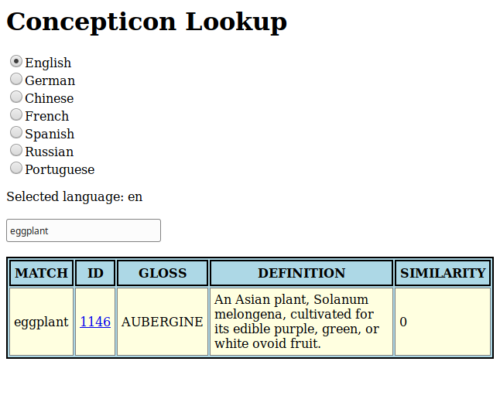
\includegraphics[width=5.20833in,height=4.15625in]{images/__f.hypotheses.org_wp-content_blogs.dir_4500_files_2019_03_Screenshot_2019-03-26-Concepticon-Lookup-eggplant-500x399.png}

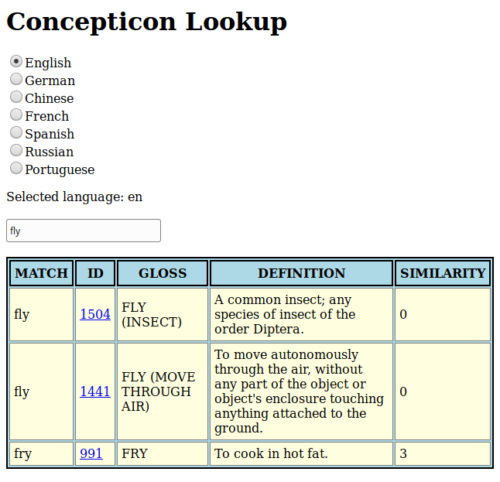
\includegraphics[width=5.20833in,height=5.02083in]{images/__f.hypotheses.org_wp-content_blogs.dir_4500_files_2019_03_Screenshot_2019-03-26-Concepticon-Lookup-fly-500x482.png}

You can see that with this application not only
\passthrough{\lstinline!eggplant!} is matched to AUBERGINE as desired,
but also that basic fuzzy matching is allowed, like in the query for
\passthrough{\lstinline!fly!} returning a list of potential mappings FLY
(INSECT), FLY (MOVE THROUGH AIR), and FRY. The output includes\\
a similarity score which we might investigate in more detail in future
posts, but in its essence the lower the score, the higher the match
probability.

This tool is a great improvement on manual searching, but it would still
be impractical for mapping entire concept lists, which usually range
anywhere from 100 to 2,500 concepts. Thankfully, we already have a set
of Python functions in pyconcepticon that allow automating this
procedure, and which can be used from the command line. Let's create a
fake concept list with different mapping issues (some clear-cut cases,
but also glosses with annotations, colexified concepts, typing errors,
etc.), which we store in a text file with one entry per line (note the
mandatory \passthrough{\lstinline!GLOSS!} column name in the first
line):

\begin{lstlisting}
GLOSS
dog
eggplant
fly (N)
to fly
hand/arm
dull
bambu
\end{lstlisting}

By running the command

\begin{lstlisting}
concepticon map_concepts conceptlist.tsv
\end{lstlisting}

we obtain the following output:

\begin{lstlisting}
GLOSS    CONCEPTICON_ID    CONCEPTICON_GLOSS    SIMILARITY
dog                2009    DOG                           2
eggplant           1146    AUBERGINE                     2
fly (N)            1504    FLY (INSECT)                  2
to fly             1441    FLY (MOVE THROUGH AIR)        1
hand/arm           2121    ARM OR HAND                   2
#<<<
dull               1518    STUPID                        2
dull                379    BLUNT                         2
#>>>
bambu               ???
#    6/7    86%
\end{lstlisting}

We can see that the method had no problem to map the five first
entries,\\
\passthrough{\lstinline!dog!} (a straightforward case),
\passthrough{\lstinline!eggplant!} (using data already mapped),
\passthrough{\lstinline!fly (N)!} (using an annotation for nouns),
\passthrough{\lstinline!to fly!} (using an annotation for verbs), and
\passthrough{\lstinline!hand/arm!} (using an annotation for
colexifications). It was not possible to decide if
\passthrough{\lstinline!dull!} should be linked to STUPID or to BLUNT
(equal similarity scores), but the items are grouped together and
clearly marked, so that review should be easy. Finally, a case of a typo
or different orthography, such as \passthrough{\lstinline!bambu!} , was
not mapped as the method does not try to be too clever, but the unmapped
item is clearly identified as such with a triple question mark (a
fall-back fuzzy string search for these cases might be implemented in
the future). The method also informs us about how many concepts were
mapped in the last line.

While glosses in English will perform better, due to its status as
default language for glosses and a consequent higher count of entries,
the same method can be used for other languages. For example, the
concept list below, in Spanish:

\begin{lstlisting}
GLOSS
perro
hombre
mujer
mano
mosca
hacer
\end{lstlisting}

can be linked with the same method by passing the
\passthrough{\lstinline!--language es!} argument to
\passthrough{\lstinline!concepticon map\_concepts!}, with the output:

\begin{lstlisting}
GLOSS    CONCEPTICON_ID    CONCEPTICON_GLOSS    SIMILARITY
perro              2009    DOG                           2
hombre             1554    MAN                           2
mujer               962    WOMAN                         2
mano               1277    HAND                          2
mosca              1504    FLY (INSECT)                  2
hacer              2575    DO OR MAKE                    2
#    6/6    100%
\end{lstlisting}

It is worth giving some notes on the inner workings of this method, also
introducing the internals aspects of Concepticon. The
\passthrough{\lstinline!map\_concepts!} command wraps a call to the
internal \passthrough{\lstinline!api.map()!} method, which will read
entries from column \passthrough{\lstinline!GLOSS!} or
\passthrough{\lstinline!ENGLISH!} and parse them with the
\passthrough{\lstinline!parse\_gloss()!} function. This helper method
offered in the pyconcepticon library is used to extract the most
important information from the \enquote{raw} gloss, along with its
annotated part-of-speech (if any), as illustrated by the code snippet
below:

\begin{lstlisting}
from pyconcepticon import glosses

for gloss in ['kill', 'kill (v)', 'to kill', 'to kill (somebody)']:
    parsed_gloss = glosses.parse_gloss(gloss)[0]
    print([gloss, parsed_gloss.main, parsed_gloss.pos])
\end{lstlisting}

Which returns:

\begin{lstlisting}
['kill', 'kill', '']
['kill (v)', 'kill', 'verb']
['to kill', 'kill', 'verb']
['to kill (somebody)', 'kill', 'verb']
\end{lstlisting}

The main part of glosses and their part-of-speech tags are used in
combination with mappings in already included concept lists, where each
\enquote{raw} gloss is aligned to Concepticon as in the snippet below (a
full list can be found
\href{https://github.com/concepticon/pyconcepticon/blob/master/tests/fixtures/mappings/map-en.tsv}{in
the repository tests} ):

\begin{lstlisting}
1504    FLY (INSECT)///FLY  1
1504    FLY (INSECT)///Fly (n.) 1
1504    FLY (INSECT)///a fly    4
1504    FLY (INSECT)///blowfly/housefly 4
1504    FLY (INSECT)///fly  16
1504    FLY (INSECT)///fly (N)  1
1504    FLY (INSECT)///fly (animal) 1
1504    FLY (INSECT)///fly (insect) 5
1504    FLY (INSECT)///fly (n)  3
1504    FLY (INSECT)///fly (n.) 2
1504    FLY (INSECT)///fly (nn.)    1
1504    FLY (INSECT)///fly (noun)   1
1504    FLY (INSECT)///fly (sb.)    1
1504    FLY (INSECT)///fly_N    1
1504    FLY (INSECT)///housefly 2
1504    FLY (INSECT)///the fly  2
1504    FLY (INSECT)///the fly (insect) 46
1504    FLY (INSECT)///the fly (insect)s    46
1441    FLY (MOVE THROUGH AIR)///(the bird) flew    1
1441    FLY (MOVE THROUGH AIR)///FLY    1
1441    FLY (MOVE THROUGH AIR)///FLY (VERB) 1
1441    FLY (MOVE THROUGH AIR)///FLY (v.)   1
1441    FLY (MOVE THROUGH AIR)///Fly    2
1441    FLY (MOVE THROUGH AIR)///TO FLY 3
1441    FLY (MOVE THROUGH AIR)///To fly 1
1441    FLY (MOVE THROUGH AIR)///fly    59
1441    FLY (MOVE THROUGH AIR)///fly (as a bird)    1
1441    FLY (MOVE THROUGH AIR)///fly (of bird)  2
1441    FLY (MOVE THROUGH AIR)///fly (to)   1
1441    FLY (MOVE THROUGH AIR)///fly (v)    4
1441    FLY (MOVE THROUGH AIR)///fly (v.)   4
1441    FLY (MOVE THROUGH AIR)///fly (vb)   3
1441    FLY (MOVE THROUGH AIR)///fly (vb.)  2
1441    FLY (MOVE THROUGH AIR)///fly [vb]   1
1441    FLY (MOVE THROUGH AIR)///fly v. 4
1441    FLY (MOVE THROUGH AIR)///fly vb 1
1441    FLY (MOVE THROUGH AIR)///fly, to    2
1441    FLY (MOVE THROUGH AIR)///fly_V  1
1441    FLY (MOVE THROUGH AIR)///flying 2
1441    FLY (MOVE THROUGH AIR)///to fly 26
1441    FLY (MOVE THROUGH AIR)///to fly (move through air)  126
1441    FLY (MOVE THROUGH AIR)///to fly / the bird flies / flew 1
1441    FLY (MOVE THROUGH AIR)///to fly away    1
\end{lstlisting}

This mapping does more than inform us that, say, the gloss
\passthrough{\lstinline!the fly (insect)!} is mapped 46 times to the
concept FLY (ANIMAL) or that \passthrough{\lstinline!to fly!} is mapped
26 times to FLY (MOVE THROUGH AIR). It also allows the algorithm to
internally parse all the different glosses for \enquote{fly} as either a
noun or a verb, so that it collects enough information to link any
different and still unobserved gloss to the correct concept. We can also
take a first glimpse at how pyconcepticon works under the hood,
preparing for future blog posts where the internals will be explored in
more detail.

Other commands in pyconcepticon might help the mapping process, such as
\passthrough{\lstinline!link!} (to link concepts to a concept set, so
that if either CONCEPTICON\_GLOSS or CONCEPTICON\_ID is given, the other
is added) and \passthrough{\lstinline!mergers!} (which prints the
Concepticon id of potential mergers), but
\passthrough{\lstinline!map\_concepts!} and
\passthrough{\lstinline!app!} are the most important ones which cannot
be lacking from your computer-assisted language comparison toolbox.

\subsection*{References}

\nopagebreak\hangindent=0.7cm {\small List, Johann Mattis \& Cysouw, Michael \& Greenhill, Simon \&
Forkel, Robert (eds.) 2018. \emph{Concepticon} . Jena: Max Planck
Institute for the Science of Human History. (Available online at
\url{http://concepticon.clld.org} , Accessed on 2019-03-26.) }

\vskip 2em
\framebox{\tabular{p{0.95\textwidth}}\textbf{Cite this article as}:
Tiago Tresoldi,
\enquote{Using pyconcepticon to
map concept lists,}
in \emph{Computer-Assisted Language Comparison in Practice},
01/04/2019, \url{https://calc.hypotheses.org/1820}.\endtabular}

\newpage
\section*{Using pyconcepticon to map concept lists (II)}
\phantomsection\addcontentsline{toc}{section}{Using pyconcepticon to map concept lists (II) (Tiago Tresoldi)}

Tiago Tresoldi (08/04/2019)

\emph{Categories}: Code

\emph{Tags}: code example, concept mapping, Concepticon, Tucanoan
languages

\begin{center}\rule{0.5\linewidth}{1pt}\end{center}

Mapping a given concept list to Concepticon can be done in a
straight-forward way, even if automatic mappings need manual refinement.
But what can we do when having to deal with larger datasets, say, a
dictionary, from which we want to extract specific concepts, such as,
for example, the ones in the classical
\href{https://concepticon.clld.org/contributions/Swadesh-1955-100}{Swadesh
list of 100 items} (Swadesh 1955)?

In the previous post on this topic, we discussed how the tools offered
by the \passthrough{\lstinline!pyconcepticon!} library, in particular,
the \passthrough{\lstinline!concepticon!} program that can be used from
the command line or with a JavaScript interface, make concept mapping
easier and more consistent. We also mentioned that they should be enough
for automating many of the tasks that make up the mapping of a concept
list to Concepticon, especially in those cases when programmers might be
tempted to come up with half-baked implementations that are not
reusable. Still, cases of one-time, dataset-specific solutions might be
desirable or even necessary, such as when dealing with difficult concept
lists that need to be pre-processed for manual intervention. While
Concepticon, as part of the CLDF standard, is composed of plain-text
files that could be loaded and manipulated with any programmer's
favorite language or approach, in most cases it makes sense to use the
internal component of the \passthrough{\lstinline!pyconcepticon!}
library, wrapping them around our functions and workflows.

Let's illustrate this with an actual example, presented step-by-step. We
recently had to start mapping a dataset for Barasana, a Tukanoan
language spoken in Colombia. We had the following issues: - Unlike most
desirable cases for computer-assisted language comparison, at least in
its more common current settings, the data does not come from lists of
basic vocabulary (usually collected with the comparative method in
mind), but from a bilingual Barasana-Spanish dictionary compiled by
Jones and Jones (2009).- The \enquote{dictionary} feature leads to two
issues: first, most of the entries are far from comparable in the sense
that they are too culture-specific or are clearly the output of word
formation processes; second, second, the definitions, while occasionally
similar to glosses, are in most cases long and complex lexicographic
definitions.- As the source is a bilingual \emph{dictionary} , and not a
bilingual \emph{wordlist} or \emph{vocabulary} , in many cases different
words in our source language (Barasana) are translated with the same
Spanish \enquote{gloss}, especially in case of common vocabulary.- The
same definitions constitute our proxy to the forms glosses, but as
mentioned they are given in Spanish, a language with less representation
in Concepticon due to the majority of the concept lists already there
using English or Mandarin for elicitation.- For the purpose of the
analysis, we did not want to map all possible concepts found in the data
and already in Concepticon, but only the essential Swadesh-100 list,
thus excluding entries with perfect matches like TELEPHONE.

Most of the issues above should be clear just from the first lines of
our raw data:

\begin{lstlisting}
$ head barasana.tsv
 SOURCE-ORTHOGRAPHY    SOURCE-PHONETIC SOURCE-WORD-CLASS   SOURCE-DEF  ENGLISH-GLOSS   DIALECT-NOTE    GRAMMAR-NOTE
 abarijʉ     ɑ́ˈbɑ.ɾi.hɨ́ E][ɑbɑ́.ˈɾí.hɨ J   s.v.inan.   cosa blanda (como tierra, fruta de árbol, coca pilada, herida, abdomen)
 abase     ɑ́ˈbɑ.se E][ɑˈbɑ́.sé J  v.i.    (ser/estar) blando, blanda (casabe, lodo)           ntg BARS,91 //aba// ‘soft’ with the stative verb //aba// ‘to be soft’ is// aba-se// ‘that which is soft’, no459; lf caus.
 abee     ɑˈbéé   interj.     ¡ay no! (exclamación de amor frustrado)             ntg BARS,91 //Abe!// ‘expression of love for someone’ p40, 2.27-2.30 Interjections, 2.29. Exclamatory;
 abi     ɑˈbí    interj.     ¡ay!            ntg BARS,91 //Abi!// ‘Oh, how small!/Oh, what a small quantity!’, p39, 2.29. Exclamatory. //Abo!// ‘oh, how big!; oh, what a huge quantity!’ is an example of an exclamatory interjection. /o/ is used iconically for ‘bigness’ and /i/ is used for ‘smallness’. Thus, //Abi//! ‘oh, how small!; oh, what a small quantity!’ We have recorded over thirty exclamatory interjections, many of which are synonymous, and most of which begin with /a/. Some of these are listed in (118);
 aboo     ɑˈbóo   interj.     ¡ah!        va abuu , ph ɑˈbúúú ,   ntg BARS,91 //Abo!// ‘Oh, how big!/Oh, what a huge quantity!’, p.39, 2.29. Exclamatory. is an example of an exclamatory interjection. o is used iconically for ‘bigness’ and i is used for ‘smallness’. Thus, //Abi!// ‘oh, how small!; oh, what a small quantity!’ We have recorded over thirty exclamatory interjections, many of which are synonymous, and most of which begin with a. Some of these are listed in (118);
 abore         v.caus.dep.     ser.blando-CAUS-nS          ntg BARS,91 //abo// (soft.CAUS) p70, no311;
 abu     ˈɑ́bu   inan.s.de masa  alga        va aburi , uv E , vn J
 aburi     ɑ́ˈbúɾí     inan.s.de masa  alga        va abu , uv J , vn E
 áburi     ˈɑ́buɾi     inan.s.de masa  zumo; jugo de yuca brava (no venenoso)
\end{lstlisting}

No acceptable automatic mapping seems possible, which makes this one
more supporting evidence for our insistence in computer- \emph{assisted}
language comparison: assisted mappings, where our algorithm does not try
to be too clever but gives enough information for an expert decision
later, \emph{are} possible. We can demonstrate how such data can be
generated, all while relying on previous work by means of the
\passthrough{\lstinline!concept\_map()!} and
\passthrough{\lstinline!concept\_map2()!} functions of
\passthrough{\lstinline!pylexibank!} (briefly mentioned in the previous
post).

While there are some differences in their inner workings, with
\passthrough{\lstinline!concept\_map()!} more a \enquote{full search}
than \passthrough{\lstinline!concept\_map2()!} , both mapping functions
work similarly, requiring two lists of strings: - The first one,
\passthrough{\lstinline!glosses!} , is a list of glosses or definitions
we want to map, as found in the source data.- The second one,
\passthrough{\lstinline!map\_reference!} , is a list of reference points
composed of Concepticon glosses and reference glosses, separated by
triple slashes \passthrough{\lstinline!"///"!} . Examples, as those
provided in the previous post and available on-line in pre-compiled
lists (such as
\href{https://github.com/concepticon/pyconcepticon/blob/master/tests/fixtures/mappings/map-en.tsv}{this}
for English), are
\passthrough{\lstinline!"FLY (INSECT)///fly (insect)"!} and
\passthrough{\lstinline!"FLY (MOVE THROUGH AIR)///fly (as a bird)"!} .

The items composing the \passthrough{\lstinline!glosses!} list can be
pre-processed by the user in terms of textual manipulations, like
removing leading and trailing spaces, or information extraction (such as
obtaining the actual gloss from definitions with comments, like
\passthrough{\lstinline!dog!} from
\passthrough{\lstinline!the dog (noun)!} ), but both functions take care
of that by default. The \passthrough{\lstinline!map\_reference!} list
can also be compiled by the user as needed, but, in most cases, we will
use \passthrough{\lstinline!pyconcepticon!} 's
\passthrough{\lstinline!\_get\_map\_for\_language()!} function, which
loads the precompiled, per-language references from concept lists mapped
in the past, allowing us to quickly stand in the shoulders of past
concept mappers.

Let's explore these data structures: we load our raw data using Python's
default \passthrough{\lstinline!csv!} library, extract the glosses with
a list comprehension, and build a reference map from the second element
of each item of the value returned by
\passthrough{\lstinline!\_get\_map\_for\_language()!} (readers are free
to explore the additional information returned by this function; the
\passthrough{\lstinline!"es"!} parameter is the language code for
Spanish, which is necessary as \passthrough{\lstinline!pyconcepticon!}
defaults to \passthrough{\lstinline!"en"!} for English).

\begin{lstlisting}
# Imports the necessary libraries
import csv
import pyconcepticon.api

# Loads the Concepticon API with data from the specified path
# NOTE: REMEMBER TO SET YOUR OWN PATH IF NECESSARY!!!
CONCEPTICON_PATH = "/home/tresoldi/src/concepticon-data"
Concepticon = pyconcepticon.api.Concepticon(CONCEPTICON_PATH)

# Loads the raw data
with open('barasana.tsv') as csvfile:
    reader = csv.DictReader(csvfile, delimiter='\t')
    data = [row for row in reader]

# Loads the full language mapping, also setting the `lang`uage
lang = "es"
spanish_map = Concepticon._get_map_for_language(lang)

# Builds lists of glosses and references, and shows some contents
glosses = [entry.get('SOURCE-DEF') for entry in data]
map_reference = [entry[1] for entry in spanish_map]
print("glosses", glosses[:5])
print("map_reference", map_reference[:5])
\end{lstlisting}

Which returns:

\begin{lstlisting}
glosses ['cosa blanda (como tierra, fruta de árbol, coca pilada, herida, abdomen)', '(ser/estar) blando, blanda (casabe, lodo) ', '¡ay no! (exclamación de amor frustrado) ', '¡ay! ', '¡ah! ']
map_reference ['ABACUS///Ábaco', 'ABSTAIN FROM FOOD///ayunar', 'ACCORDION///Acordeón', 'ACCUSE///acusar, denunciar', 'ACHIOTE///achiote, bija']
\end{lstlisting}

We can now obtain the automatic mapping for each gloss, by calling
either \passthrough{\lstinline!concept\_map()!} or
\passthrough{\lstinline!concept\_map2()!} on the
\passthrough{\lstinline!glosses!} list (from which we first remove any
empty glosses); the differences between the methods will be explained in
a future post, but it should be enough to know that they are essentially
interchangeable, both returning a dictionary with the indexes in
\passthrough{\lstinline!glosses!} as the keys and a tuple with the list
of matched entries in \passthrough{\lstinline!map\_reference!} and the
similarity score as the values (
\passthrough{\lstinline!concept\_map2()!} return all entries with a
similarity score lower than the requested one). Such formal description
might be a bit unintuitive, so let's demonstrate with code:

\begin{lstlisting}
# Import the functions for the mapping
from pyconcepticon.glosses import concept_map, concept_map2

# Remove empty glosses
glosses = [gloss for gloss in glosses if gloss]

# Perform the mapping and show some of the entries (if they are found,
# otherwise print `None`)
mapping = concept_map(glosses, map_reference, language=lang, similarity_level=5)
for i in range(5):
    print([i, glosses[i], mapping.get(i, None)])
\end{lstlisting}

And, especially, with its results (also noting as some definitions, here
\enquote{glosses}, are not mapped as the algorithm is unable to find an
acceptable match with the similarity range we requested), below. The
first entry, \passthrough{\lstinline!([1757], 4)!} , means that a single
match, of index 1757 and similarity score of 4, was found for the gloss
starting with \passthrough{\lstinline!cosa blanda...!} ; gloss of
indexes 2 to 4, all interjections such as \passthrough{\lstinline"¡ay!"}
, had no match.

\begin{lstlisting}
[0, 'cosa blanda (como tierra, fruta de árbol, coca pilada, herida, abdomen)', ([1757], 4)]
[1, '(ser/estar) blando, blanda (casabe, lodo) ', ([978], 4)]
[2, '¡ay no! (exclamación de amor frustrado) ', None]
[3, '¡ay! ', None]
[4, '¡ah! ', None]
\end{lstlisting}

As humans, we prefer textual representations to indexes of list indexes.
The code should do us the heavy and boring work of mapping the latter to
the former, so we collect the matched glosses by iterating over the
\passthrough{\lstinline!mapping!} dictionary and extracting the part of
the \passthrough{\lstinline!reference!} string found before the
\passthrough{\lstinline!"///"!} delimiter--- note that we do so by
setting a default value \passthrough{\lstinline!([], None)!}, which
indicates no matched concepts (its first element is an empty list) and,
consequently, no similarity score (thus, \passthrough{\lstinline!None!}
). As the list of matched elements will likely have repeated elements
(because more than one reference gloss might be matched, and those will
likely share their Concepticon ID), we also take a
\passthrough{\lstinline!set!} of the elements before storing the results
we care about in \passthrough{\lstinline!mapped\_glosses!} . This
programming logic could be done in a single Python list comprehension,
but it is better to proceed stepwise here and collect each gloss match
within a \passthrough{\lstinline!for!} loop.

\begin{lstlisting}
# Collect matched glosses and show some of them
mapped_glosses = {}
for gloss_idx, gloss in enumerate(glosses):
    match_idxs, sim = mapping.get(gloss_idx, ([], None))

    match_glosses = set([
        map_reference[match_idx].split('///')[0]
        for match_idx in match_idxs
    ])

    mapped_glosses[gloss] = list(match_glosses)

for item in sorted(mapped_glosses.items())[:10]:
    print(item)
\end{lstlisting}

The output shows that our code works and, once more, that most
definitions will \emph{not} be mapped.

\begin{lstlisting}
('(año, semana) pasado', [])
('(estar) abierto, abierta', [])
('(estar) agotado, agotada (persona, animal) ', ['ANIMAL'])
('(estar) agotado, agotada (personas, animales) ', [])
('(estar) agotado, agotada (una persona, un animal) ', [])
('(estar) agrio, agria (limón, lulo, casabe hecho del almidón guardado por demasiado tiempo) ', ['SOUR'])
('(estar) alerto, alerta; ', [])
('(estar) apretado, apretada ', [])
('(estar) arrugada ', [])
('(estar) atrancado, atrancada; ', [])
\end{lstlisting}

At this point, we have our automatic mapping of all lexicographic
definitions in the source as a list of potential matches in Concepticon
with no, one, or multiple elements. We now need to filter only the
entries with potential matches in the Swadesh 100 list.

As mentioned earlier, given that Concepticon data is stored in
plain-text files, we could just read the raw
\passthrough{\lstinline!concepticon-data/concepticondata/conceptlists/Swadesh-1964-100.tsv!}
file and collect all its gloss under the
\passthrough{\lstinline!CONCEPTICON\_GLOSS!} column. However,
\passthrough{\lstinline!pyconcepticon!} already has functions in place
for iterating over the properties of a concept list, so that it is
easier and faster for us to just wrap it in our own code. Considering
that we need to perform some checks and operations, and especially that
such code might be useful in the future, we can write our own function
for collecting the glosses of an existing concept list.

\begin{lstlisting}
# Define a function for obtaining the glosses of a concept list
def glosses_from_list(list_id):
    """
    Returns a list with the Concepticon glosses for a given conceptlist.

    Takes care of removing duplicates, empty entries, etc.

    Parameters
    ----------
    list_id : str
        The unique identifier for the list, as used in Concepticon, such
        as "Swadesh-1964-100".
    """

    # Obtain the concept list with a list comprehension; note the [0]
    # subsetting for getting the first element of the comprehension
    concept_list = [
        cl for cl in Concepticon.conceptlists.values()
        if cl.id == list_id
    ][0]

    # Obtain all the Concepticon glosses in the list; remember that they
    # glosses might be duplicated or empty at this point
    glosses = [
        concept.concepticon_gloss for concept
        in concept_list.concepts.values()
    ]

    # Remove any empty (i.e., non mapped) glosses and make sure there are
    # no duplicates (using `set`)
    glosses = set([gloss for gloss in glosses if gloss])

    # Return as a list
    return sorted(glosses)

# Obtain the glosses from the Swadesh 100 list and show some of them
swadesh = glosses_from_list("Swadesh-1964-100")
print(swadesh[:10])
\end{lstlisting}

Which works as expected:

\begin{lstlisting}
['ALL', 'ASH', 'BARK', 'BELLY', 'BIG', 'BIRD', 'BITE', 'BLACK', 'BLOOD', 'BONE']
\end{lstlisting}

We are now ready to generate our results, iterating over the data we
collected earlier and writing to a
\passthrough{\lstinline!barasana-swadesh.tsv!} file the rows that hold
potential Swadesh entries. A better output than the one coded below
could be provided, making the reviewing task even easier--- for example,
by sorting entries by similarity score, listing glosses alphabetically,
or already including the Concepticon ID. However, this should be easy to
any Python programmer and is beyond our scope of illustrating the inner
working of \passthrough{\lstinline!pyconcepticon!} .

\begin{lstlisting}
# Write the output
with open('barasana-swadesh.tsv', 'w') as handler:
    # Write headers
    handler.write('FORM\tPHONETIC\tDEFINITION\tGLOSSES\tNOTES\n')

    # Iterate over all rows looking for potential Swadesh data
    for row in data:
        # Extract the list of glosses per form, defaulting to an empty list
        glosses = mapped_glosses.get(row['SOURCE-DEF'], [])

        # Get the subset of glosses that are in Swadesh 100
        glosses = [gloss for gloss in glosses if gloss in swadesh]

        # If there is at least one Swadesh gloss, build a buffer from the
        # row, adding an information on all potential glosses (separated with a
        # vertical bar in case of multiple glosses), and print it
        if glosses:
            buf = [
                row['SOURCE-ORTHOGRAPHY'],
                row['SOURCE-PHONETIC'],
                row['SOURCE-DEF'],
                '|'.join(glosses),
                row['GRAMMAR-NOTE'],
            ]

            handler.write('%s\n' % '\t'.join(buf))
\end{lstlisting}

We can finally inspect the results and confirm that the code is working,
such as in good potential matches as \lstinline!ãmo! for
HAND and \lstinline!baáre! for EAT. We can already spot
problems, as well: \lstinline!adocʉ̃! was mapped to PERSON
due to the parsing of its definition, and
\lstinline!baásãare! , clearly a word formation including
the \lstinline!baáre! above, is also mapped to EAT (which
was expected in our logic, as both have the same Spanish gloss
\enquote{comer}). Nevertheless, we surely saved a lot of time for the
linguists that would correct this first mapping, also gaining much in
terms of consistency. Even better, once the results will be finished and
included in Concepticon, the new concept list from Barasana with Spanish
definitions will improve the results for future semi-automatic and
automatic mappings, especially in case of other datasets with glosses in
Spanish (thus helping, for example, to include more Native American
Languages in Lexibank).

\begin{lstlisting}
$ head barasana-swadesh.tsv
 FORM    PHONETIC    DEFINITION  GLOSSES NOTES
 adocʉ̃     ɑˈdó.kɨ̃́   este tamaño de (animal, persona)    PERSON
 ãmo     ˈɑ̃́mõ E][ˈɑ̃́mṍ J  mano    HAND
 ãmʉa     ɑ̃́ˈmɨ̃ɑ̃ E][ˈɑ̃́mɨ̃́ɑ̃́ J  cuello (ser humano, botella)    NECK
 ãmʉtutu     ɑ̃́mɨ̃.tuˈtú E][ɑ̃́mˈɨ̃́.tútu J     cuello (ser humano, botella)    NECK
 baare     ˈbɑ́ɑ́.ɾe E][ˈbɑ́ɑ́.ɾé J    nadar   SWIM
 baáre     ˈbɑɑ́.ɾe    comer   EAT ntg BARS,91 //ba// ‘eat’ no4;
 baásãare     ˈbɑɑ́.sɑ̃́ɑ̃́.ɾẽ E][ˈbɑɑ́.sɑ̃́ɑ̃.ɾẽ J   comer   EAT
 bajirocare     bɑˈhí.ɾókɑ.ɾe   morir (una persona)     DIE ntg BARS,91 p.23, 2.4. Verbs with only a subject argument, p.24,  Verbs which agree in number with the subject. A very productive verb used in verb compounds, both transitive and intransitive, is roka 'to move down/away (s)'; roka becomes rea  with plural subjects. For example, baji roka 'to die (s)' and baji rea 'to die (p)';
 boagʉ, boago     ˈbóɑ́.gɨ    (ser/estar) podrido, podrida (animal, persona)  PERSON
\end{lstlisting}

The entire source code here developed is available at \href{URL}{this
GitHub Gist} .

\subsection*{References}

\nopagebreak\hangindent=0.7cm {\small Barasana Literacy Committee, Paula S. Jones and Wendell H. Jones
(compilers). 2009. \emph{Diccionario bilingüe: Eduria \&
Barasana-Español, Español-Eduria \& Barasana} . Bogotá, D.C.: Editorial
Fundación para el Desarrollo de los Pueblos Marginados. 613pp. }

\nopagebreak\hangindent=0.7cm {\small Swadesh, M. (1955): Towards greater accuracy in lexicostatistic
dating. International Journal of American Linguistics. 21.2. 121-137. }

\vskip 2em
\framebox{\tabular{p{0.95\textwidth}}\textbf{Cite this article as}:
Tiago Tresoldi,
\enquote{Using pyconcepticon to
map concept lists (II),}
in \emph{Computer-Assisted Language Comparison in Practice},
08/04/2019, \url{https://calc.hypotheses.org/1844}.\endtabular}


\newpage
\section*{Behind the Sino-Tibetan Database of Lexical
Cognates: Introductory remarks}
\phantomsection\addcontentsline{toc}{section}{Behind the Sino-Tibetan Database of Lexical
Cognates: Introductory remarks (Johann-Mattis List)}

Johann-Mattis List (13/05/2019)

\emph{Categories}: Primer

\emph{Tags}: data curation, database, EDICTOR, lexical cognates,
lexicostatistics

\begin{center}\rule{0.5\linewidth}{1pt}\end{center}

One of the major efforts behind our recently published paper on the
\href{https://www.pnas.org/content/early/2019/04/30/1817972116}{origin
and spread of the Sino-Tibetan languages} (
\href{http://bibliography.lingpy.org?key=Sagart2019}{Sagart et al.~2019}
) was the creation of a database of lexical cognates which was used to
run the phylogenetic analyses. The creation of this database started
about four years ago, when I joined the Centre des Recherches
Linguistiques sur l'Asie Oriental in Paris as a research fellow in
January 2015, and Guillaume Jacques and Laurent Sagart approached me
with the idea of making a phylogenetic study of Sino-Tibetan languages.
In December 2017, almost three years after having started, our database
consisted of 180 concepts translated into 50 different languages. Since
creating the database was not directly straightforward from the
beginning, with quite a few situations in which we realized we had to
re-arrange the data or the procedure, I thought it might be useful to
share our experience in a series of blog posts, as it might be
interesting for scholars who wish to create their own database.

A database of lexical cognates is nothing else than a comparative
wordlist in which cognate relations between words from different
languages are annotated. For the database itself, no specific software
is needed, and spreadsheet editors like LibreOffice, Excel, or Google
Sheets can easily be used for this purpose. As a minimal requirement,
such a database provides information on how a given \emph{language}
expresses a given \emph{concept} and with which other \emph{words} the
word denoting this concept in the language is etymologically related.
Ideally, more information should be supplied, of course, for example,
regarding the source of information (be it a reference or original
fieldwork), if the word has been borrowed or not, or how the word is
pronounced. If one wants to be very detailed, one can also indicate who
made the respective cognate judgments, or even supply alignments that
indicate where the experts think that the words are cognate.

While it sounds rather straightforward to create such a database at a
first glance, there are many pitfalls one should better be aware of
before starting to build one from scratch. There is a large amount of
potential problems one can encounter during the creation process. It can
turn out that the data for a key language is insufficient, key
collaborators may leave the project, coding data may turn out to require
much more time than estimated, and the results may also be disappointing
in the end.

In order to be prepared for what can happen, it would be ideal, if we
had some kind of a guideline on how to create datesets of lexical
cognates. Given large projects of datasets that were prominently used in
the past, such as \href{https://abvd.shh.mpg.de}{ABVD} (
\href{http://bibliography.lingpy.org?key=Greenhill2008}{Greenhill et al.
2008} ), IELex ( \href{http://bibliography.lingpy.org?key=Dunn2012}{Dunn
et al.~2012} ), or the datasets published as part of the
\href{http://starling.rinet.ru/new100/}{Global Lexicostatistical
Database} project (
\href{http://bibliography.lingpy.org?key=Starostin2011}{Starostin and
Krylov 2011} ), one might even think that this problem has been
discussed long enough, so that scholars who want to build a new database
on their own should not have a hard time to find enough guidance on how
to get started. Unfortunately, when going from theory to practice, our
own experience in working with lexical data from different scholars as
part of large data aggregation projects like CLICS² (
\href{http://bibliography.lingpy.org?key=List2018f}{List et al. 2018} )
has shown that this is usually not the case. While fieldworkers have
their \href{https://software.sil.org/toolbox/}{toolbox} to create
dictionaries, there is no equivalent for historical linguists working on
comparative databases of lexical cognates. As a result, scholars who
start datasets from scratch often reinvent many wheels, and the wheels
they reinvent may be squared at times.

Our experience with building the
\href{https://dighl.github.io/sinotibetan}{Sino-Tibetan Database of
Lexical Cognates} underlying the study by
\href{http://bibliography.lingpy.org?key=Sagart2019}{Sagart et
al.~(2019)} does not solve these problems. We were making use of tools
like \href{http://tsv.lingpy.org}{EDICTOR} (
\href{http://bibliography.lingpy.org?key=List2017d}{List 2017} ), which
facilitate the process of cognate coding and making alignments of the
data, but in order to get the data in a first instance, we mostly relied
on the fact that we had people (mostly also myself) in our team who
could quickly prepare custom scripts to parse available data and extract
the data we needed. We also profited much from the fact that some
projects, especially \href{http://stedt.berkeley.edu/}{STEDT} (
\href{http://bibliography.lingpy.org?key=Matisoff2015}{Matisoff 2015} ),
but also \href{http://starling.rinet.ru/}{Tower of Babel} , had been
digitizing large amounts of data in a rather regular form in the past.
We were also lucky to have people in our team who have done original
fieldwork (which enabled them to quickly fill in a list of certain
varieties, consulting informants where data was missing), and to have
external collaborators who generously shared their data and answered our
queries on specific items (see the list of acknowledgments in Sagart et
al.~2019 for details).

The way in which we assembled the data for our study was not
straightforward, but rather a winding road of many dead-ends, some
surprises, lots of discussions, some disappointments, and a lot of
lessons we learned for the future. We did not reach our (or maybe
preliminary my) initial goal of providing a database of cognates that
would provide fully aligned cognate sets and list all correspondence
patterns in an indisputable way, so that it could be inspected,
challenged, and improved by our colleagues in all kind of details one
could think of as a historical linguist. But we achieved to provide a
dataset of 180 concepts translated into 50 different varieties of
Sino-Tibetan, along with an interface to easily inspect the data which
goes beyond many of the datasets that have been published in the past.

Our data is open, scholars can easily inspect it in detail from its
\href{https://dighl.github.org/sinotibetan}{URL} , and they can even
correct the cognate judgments, add alignments, and further expand or
correct it. In order to do so, however, one needs to learn a bit about
the way in which we (1) assembled the data, (2) coded the data, and (3)
how the tools for data curation and annotation can be used. In order to
make it easier to understand what was going on \emph{behind} the
\emph{Sino-Tibetan Database of Lexical Cognates,} we plan to write a
couple of blog posts in which we will explain how the data was
assembled, curated, and analyzed.

\subsection*{References}

\nopagebreak\hangindent=0.7cm {\small Dunn, Michael (2012): Indo-European lexical cognacy database
(IELex). \href{//ielex.mpi.nl/”}{http://ielex.mpi.nl/} }

\nopagebreak\hangindent=0.7cm {\small Greenhill, Simon J. and Blust, Robert and Gray, Russell D. (2008):
The Austronesian Basic Vocabulary Database: From bioinformatics to
lexomics. \emph{Evolutionary Bioinformatics} 4. 271-283. }

\nopagebreak\hangindent=0.7cm {\small List, Johann-Mattis (2017): A web-based interactive tool for
creating, inspecting, editing, and publishing etymological datasets. In:
Proceedings of the 15th Conference of the European Chapter of the
Association for Computational Linguistics. System Demonstrations.
9-12. }

\nopagebreak\hangindent=0.7cm {\small List, Johann-Mattis and Simon Greenhill and Cormac Anderson and
Thomas Mayer and Tiago Tresoldi and Robert Forkel (eds.) (2018): CLICS:
Database of Cross-Linguistic Colexifications. Max Planck Institute for
the Science of Human History. Jena:
\href{//clics.clld.org/”}{http://clics.clld.org/} . }

\nopagebreak\hangindent=0.7cm {\small Matisoff, James A. (2015): The Sino-Tibetan Etymological Dictionary
and Thesaurus project. Berkeley:University of California. }

\nopagebreak\hangindent=0.7cm {\small Sagart, Laurent and Jacques, Guillaume and Lai, Yunfan and Ryder,
Robin and Thouzeau, Valentin and Greenhill, Simon J. and List,
Johann-Mattis (2019): Dated language phylogenies shed light on the
ancestry of Sino-Tibetan. \emph{Proceedings of the National Academy of
Science of the United States of America} . 1-6. DOI:
\href{https://doi.org/10.1073/pnas.1817972116}{10.1073/pnas.1817972116} }

\nopagebreak\hangindent=0.7cm {\small Starostin, George S. and Krylov, Phil (eds.) (2011): The Global
Lexicostatistical Database. Compiling, clarifying, connecting basic
vocabulary around the world: From free-form to tree-form.
\href{//starling.rinet.ru/new100/main.htm”}{http://starling.rinet.ru/new100/main.htm}. }

\vskip 2em
\framebox{\tabular{p{0.95\textwidth}}\textbf{Cite this article as}:
Johann-Mattis List,
\enquote{Behind the
Sino-Tibetan Database of Lexical Cognates: Introductory remarks,}
in \emph{Computer-Assisted Language Comparison in Practice},
13/05/2019,
\url{https://calc.hypotheses.org/1882}.\endtabular}


\newpage
\section*{Biological metaphors and methods in
historical linguistics (1): Introduction}
\phantomsection\addcontentsline{toc}{section}{Biological metaphors and methods in
historical linguistics (1): Introduction (Nathanael E. Schweikhard)}

Nathanael E. Schweikhard (15/05/2019)

\emph{Categories}: Methodology

\emph{Tags}: biology, discussion, interdisciplinary research, metaphors,
methodological transfer

\begin{center}\rule{0.5\linewidth}{1pt}\end{center}

Evolutionary biology and historical linguistics share a long history of
scientific exchange, reflected both not only in the sharing and transfer
of metaphors but more recently also in the transfer of methods. Already
Charles Darwin claimed that both species and languages evolve in
tree-like patterns, and linguists, like Wilhelm Meyer-Lübke, used terms
like \enquote{sprachliche{[}n{]} Biologie} (\enquote{linguistic
biology}) when referring to the history of languages (Meyer-Lübke 1890,
x). While the discipline of historical-comparative linguistics allowed
biologists to adopt evolutionary thought against religious dogma in the
late 19th century (Wells 1987: 54), it was biological applications which
opened up the possibility of large quantitative studies in linguistics
based on computational approaches (Geisler and List 2013, 111).

Many articles and essays have been written listing possible similarities
between the disciplines (for recent ones see for example Pagel 2016 or
List et al.~2016). Yet biology is considered a natural science, while
linguistics is thought to belong to the humanities. One could even say
that their research objects belong to two different worlds, the
objective universe, on the one hand, and the world of the products of
the subjective mind, on the other hand (Geisler and List 2013: 121).
Therefore, one may rightfully ask what it is that makes the exchange of
ideas so fruitful.

Both disciplines deal with historical processes and can therefore be
seen as belonging to the wider field of historical sciences which are
dealing with the past and how it lead to the present by
\enquote{analyz{[}ing{]} persistence with modification of systems
(\enquote{descent with modification})} (Stevick 1963, 160). In other
words, they describe and reconstruct earlier stages of their research
objects, proposing ancestral character states in biology or proto-forms
in linguistics (Atkinson and Gray 2005, 519), or investigate earlier
stages directly, where they are still attested as fossils or in form of
manuscripts and inscriptions (ibid: 514). Additionally, both disciplines
propose theories that seek to explain the transmission of their research
objects, be it vertical (in form of inheritance) or horizontal (in form
of direct exchange).

Change in linguistics and biology can be studied from different
perspectives. One can restrict oneself to study only one language or
species at the same time, investigating its internal history from its
oldest attestations to the present, or one can compare several languages
or species, which form a family, and investigate how they separated and
interacted after separation.

In addition, one can also carry out a general comparison of languages
and species in order to find the general laws and tendencies by which
they change, which is part of the typologogical approach in linguistics.
Both fields are thus based on the assumption that all languages and
species change through time. Already August Schleicher stated that
\enquote{Sprachen sich verändern so lange sie leben} (Schleicher 1863:
18, \enquote{Languages change as long as they are alive}). There is some
debate among scholars as to whether the principles of change might also
change with time or whether they remain constant.

Considering these similarities, but also the obvious differences between
the fields, looking at historical linguistics against the contrast of
evolutionary biology is of particular benefit when modeling language
history as it forces one to be explicit about one's assumptions. This
inspired us to start a series of blogposts on comparisons between
biology and linguistics. In future posts we will describe in more detail
which correspondences and differences there are between the research
objects of biology and linguistics and what needs to be taken into
account when using methods from evolutionary biology to tackle problems
in historical linguistics.

\subsection*{References}

\nopagebreak\hangindent=0.7cm {\small Atkinson, Quentin D., and Russell D. Gray. 2005. \enquote{Curious
Parallels and Curious Connections: Phylogenetic Thinking in Biology and
Historical Linguistics.} \emph{Systematic Biology} 54 (4): 513--26.
\url{http://www.jstor.org/stable/20061257} . }

\nopagebreak\hangindent=0.7cm {\small Geisler, H., and J.-M. List. 2013. \enquote{Do Languages Grow on
Trees? The Tree Metaphor in the History of Linguistics.} In
\emph{Classification and Evolution in Biology, Linguistics and the
History of Science. Concepts-- Methods -- Visualization} , edited by
Heiner Fangerau, Hans Geisler, Thorsten Halling, and William Martin,
111--24. Stuttgart: Franz Steiner Verlag. }

\nopagebreak\hangindent=0.7cm {\small Gray, Russell D., Simon J. Greenhill, and Malcolm D. Ross. 2007.
\enquote{The Pleasures and Perils of Darwinzing Culture (with
Phylogenies).} \emph{Biological Theory} 2 (4): 360--75. }

\nopagebreak\hangindent=0.7cm {\small List, Johann-Mattis, Jananan Sylvestre Pathmanathan, Philippe Lopez,
and Eric Bapteste. 2016. \enquote{Unity and Disunity in Evolutionary
Sciences: Process-Based Analogies Open Common Research Avenues for
Biology and Linguistics.} \emph{Biology Direct} , nos. 39, 11: 1--17. }

\nopagebreak\hangindent=0.7cm {\small Meyer-Lübke, Wilhelm. 1890. \emph{Italienische Grammatik} . Leipzig:
Verlag von O. R. Reisland. }

\nopagebreak\hangindent=0.7cm {\small Pagel, Mark. 2016. \enquote{Darwinian Perspectives on the Evolution
of Human Languages.} \emph{Psychonomic Bulletin \& Review} , 1--7.
\url{https://doi.org/10.3758/s13423-016-1072-z} . }

\nopagebreak\hangindent=0.7cm {\small Schleicher, August. 1863. {]} {[} \emph{Die darwinsche Theorie und
die Sprachwissenschaft} . Weimar: Hermann Böhlau. }

\nopagebreak\hangindent=0.7cm {\small Stevick, Robert D. 1963. \enquote{The Biological Model and
Historical Linguistics.} \emph{Language} , nos. 2, 39: 159--69.
\url{https://www.jstor.org/stable/411199} . }

\nopagebreak\hangindent=0.7cm {\small Wells, Rulon S. 1987. \enquote{The Life and Growth of Language:
Metaphors in Biology and Linguistics.} In \emph{Biological Metaphor and
Cladistic Classification: An Interdisciplinary Perspective; {[}Papers
from Symposium on Biological Metaphor Outside Biology (1982.03.04-05,
Philadelphia) Interdisciplinary Round-Table on Cladistics and Other
Graph Theoretical Representations (1983.04.28-29, Philadelphia){]}} ,
edited by Henry Max Hoenigswald, 39--80. Philadelphia: Univ. of
Pennsylvania Pr. }

\vskip 2em
\framebox{\tabular{p{0.95\textwidth}}\textbf{Cite this article as}:
Nathanael E. Schweikhard,
\enquote{Biological
metaphors and methods in historical linguistics (1): Introduction,}
in \emph{Computer-Assisted Language Comparison in Practice},
15/05/2019,
\url{https://calc.hypotheses.org/1866}.\endtabular}


\newpage
\section*{Rooting MADness}
\phantomsection\addcontentsline{toc}{section}{Rooting MADness (Gerhard J\"{a}ger)}

Gerhard J\"{a}ger (22/05/2019)

\emph{Categories}: Analysis

\emph{Tags}: phylogenetic reconstruction, rooting

\begin{center}\rule{0.5\linewidth}{1pt}\end{center}

\leavevmode\hypertarget{write}{}%
Rooting of phylogenetic trees is an important task, not only in
evolutionary biology, but also in historical linguistics. So far,
however, different rooting methods have not yet been sufficiently tested
on linguistics data. Given that a new method for the automatic rooting
of phylogenetic trees has been presented recently in biology, it seemed
to be a good occasion to test in detail how well this new method works
in comparison with alternative methods.

{A few months ago, Mattis List pointed my attention to a (relatively)
novel method for rooting phylogenetic trees with branch lengths:
\emph{Minimal Ancestor Deviation} rooting (Kümmel Tria et al.~2017). I
will not go into the details of that algorithm here; the interested
reader is referred to the mentioned article. Suffice it to give two
quotations:}

\begin{quote}
{\emph{\enquote{The MAD method operates on binary unrooted trees and
assumes that branch lengths are additive and that OTUs are
contemporaneous.} (Kümmel Tria et al.~2017:1)}}
\end{quote}

{and}

\begin{quote}
{\emph{Branch ancestor deviations quantify the departure from strict
clock-like behaviour, reflecting the level of rate heterogeneity among
lineages. Wrong positioning of the root will lead to ­erroneous iden-
tification of ancestor nodes, and apparent deviations will tend to be
larger. We therefore infer the MAD root as the branch and position that
minimizes the ancestor deviation {[}\ldots{}{]}. (Kümmel Tria et al.
2017: 2)}}
\end{quote}

{Several standard algorithms for phylogenetic infernce (e.g., Neighbor
Joining, most off-the-shelf implementations of Maximum Likelihood)
produce unrooted trees with branch lengths, and one needs to perform
rooting as a separate step. So if this new kid in town is better than
standard techniques such as midpoint rooting or outgroup rooting, this
might come in handy.}

{Mattis and me were interested in how well this method performs in
comparison to other rooting methods when applied to language trees
derived from word lists. So I did a little experiment.}

{In Jäger (2018), I describe a method to apply automatic cognate
detection to the data from the \href{https://asjp.clld.org/}{ASJP
project} (Wichmann et al.~2016), to extract character matrices and to
apply Maximum Likelihood (ML) phylogenetic inference (Data and code are
available at \url{https://osf.io/cufv7/} ). In the meantime I have
updated my database to ASJP v. 18. I used those data to infer ML trees
for all Glottolog families for which ASJP contains at least 10
contemporaneous doculects, using the Glottolog classification as
constraint tree. This gave me 64 unrooted trees. (To my dismay, I
noticed along the way that the Glottolog classification that is shipped
with ASJP is incomplete, so I extracted the Glottolog classification
from the Glottolog website.)}

{I will use
\href{https://glottolog.org/resource/languoid/id/nduu1242}{Ndu} (a
language family spoken in Papua New Guinea; traditionally considered as
part of the Sepik family) as my running example. The Glottolog
classification looks like this:}

{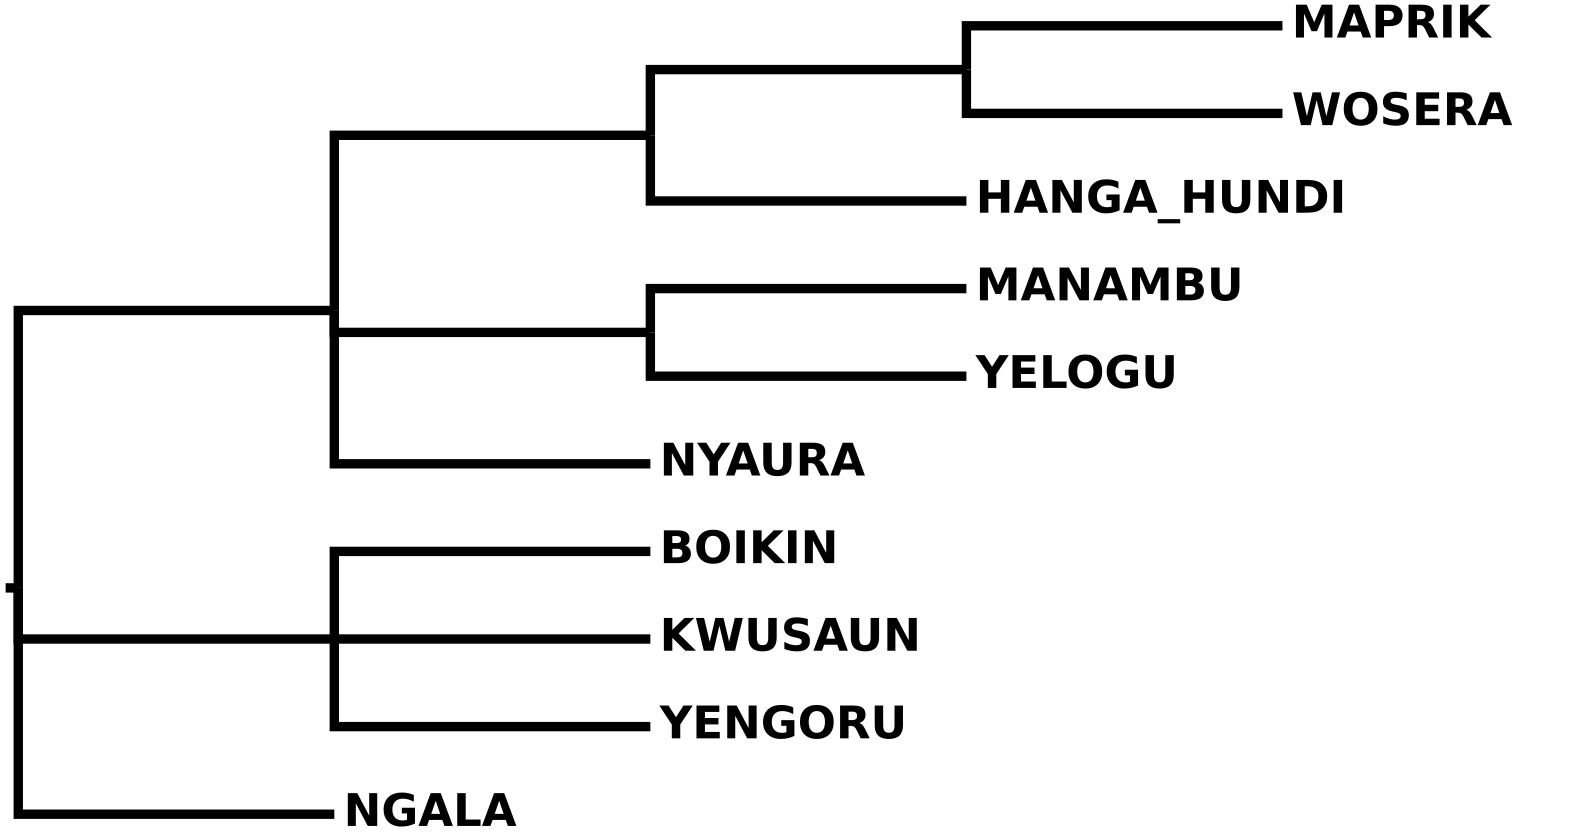
\includegraphics[width=5.21875in,height=2.78125in]{images/Ndu.glot.jpg}}

{My ML-tree (obtained using the great software
\href{https://cme.h-its.org/exelixis/web/software/raxml/index.html}{RAxML}
) is here:}

{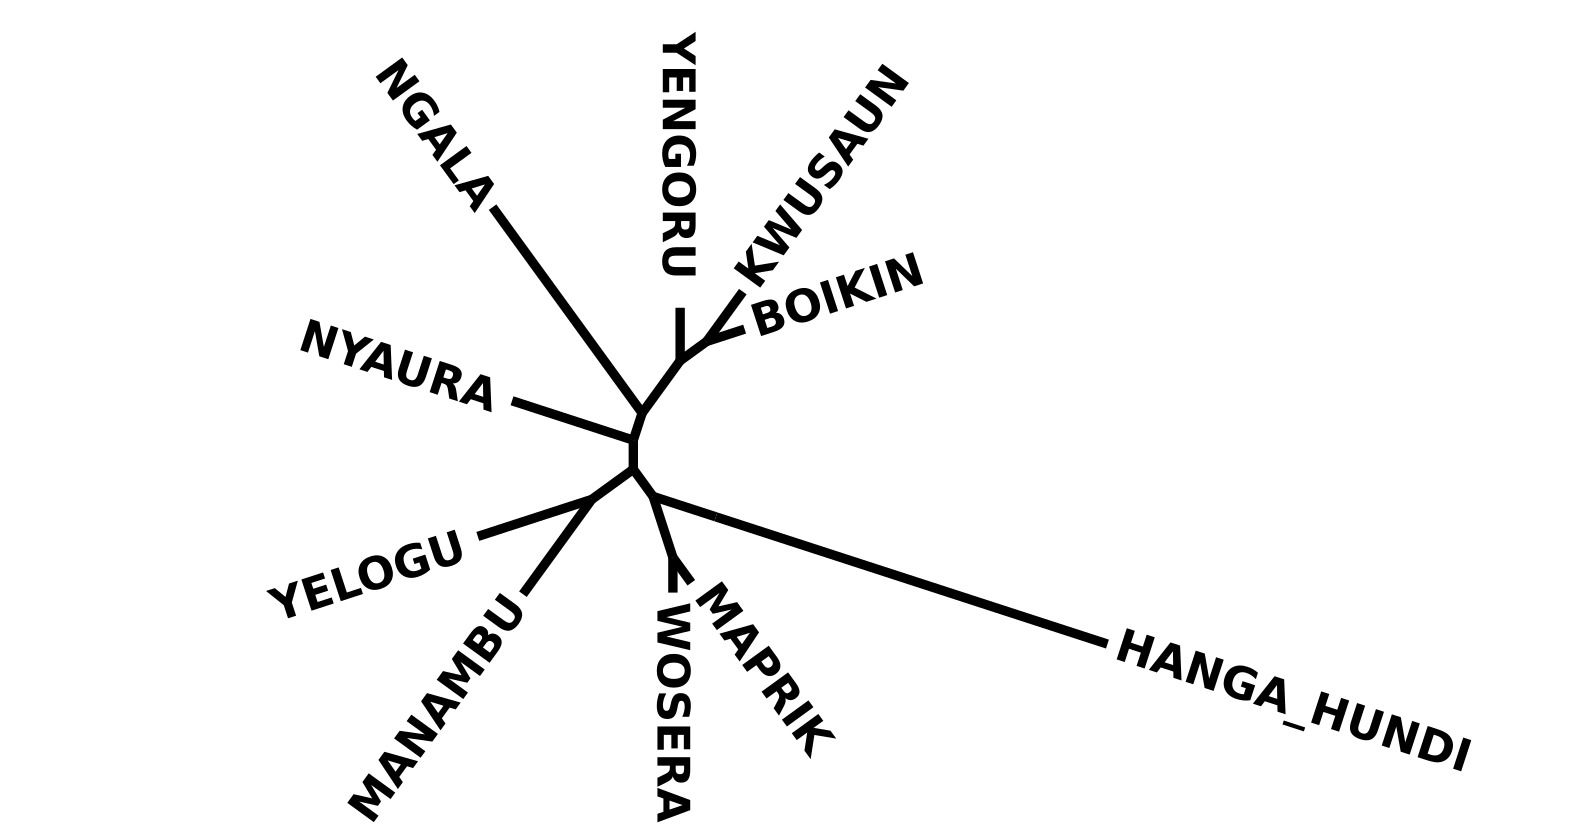
\includegraphics[width=5.21875in,height=2.78125in]{images/Ndu.unrooted.jpg}}

{The task is to find the correct root of the unrooted tree. However, the
goldstandard does not identify a unique root, as Glottolog identifies
three subgroups (Boikin, Ngala, and Nuclear Ndu).}

{Consider, e.g., the midpoint-rooted version of the ML tree:}

{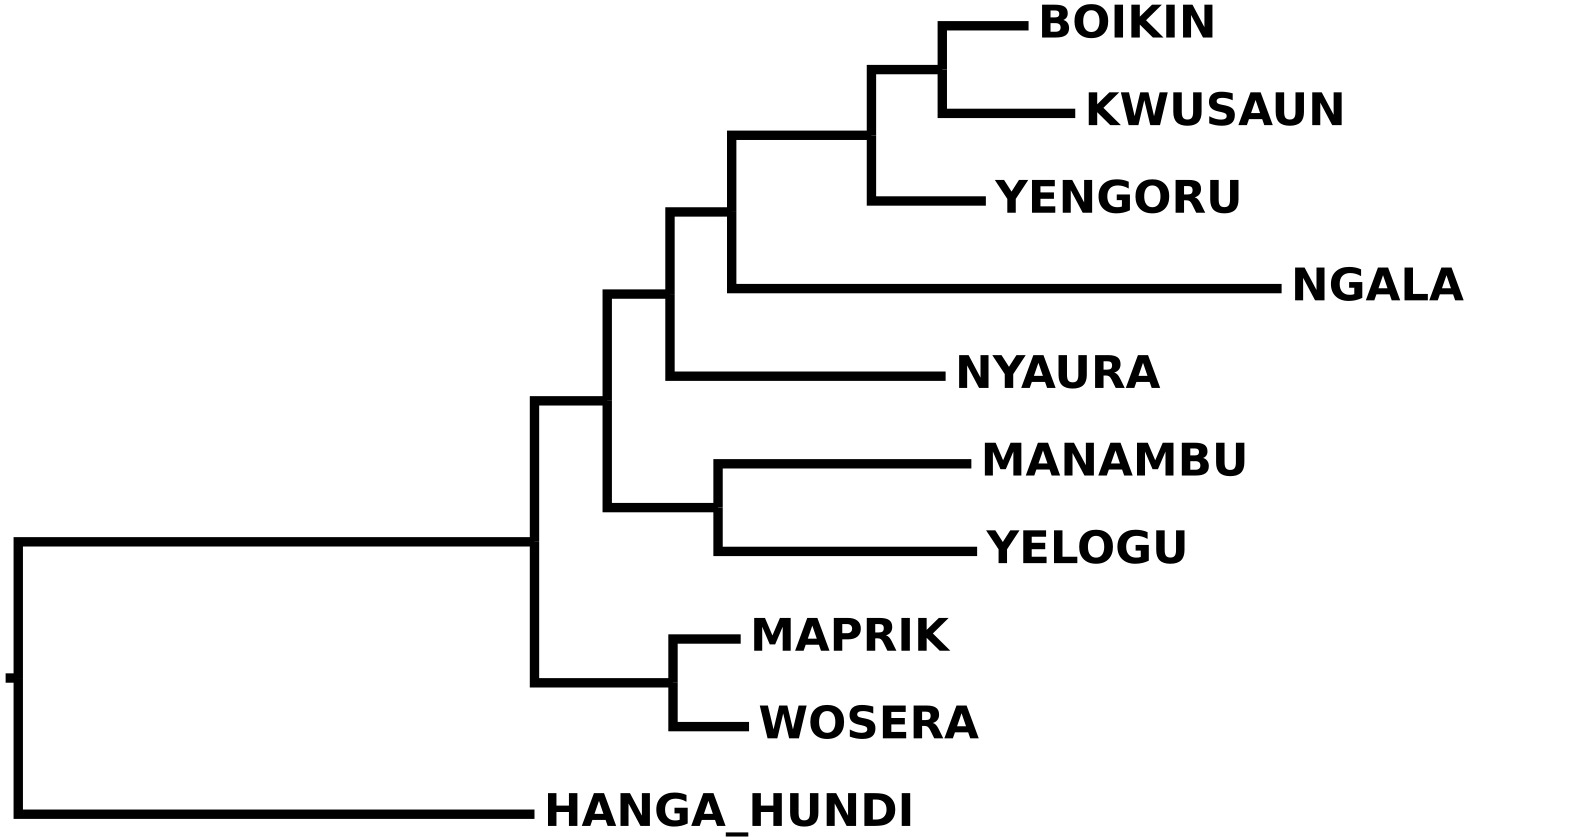
\includegraphics[width=5.21875in,height=2.78125in]{images/Ndu.midpointRooted.jpg}}

{This looks pretty bad, but can we quantify how bad it is?}

{One way to do it is to harness the \emph{triplet distance} (Sand et al.
2014) between the rooted tree and the Glottolog goldstandard.}

{To see what this is about, consider the triplet (Yengoru, Yelogu,
Wosera). In the goldstandard tree, it is grouped as (Yengoru, (Yelogu,
Wosera)).}

{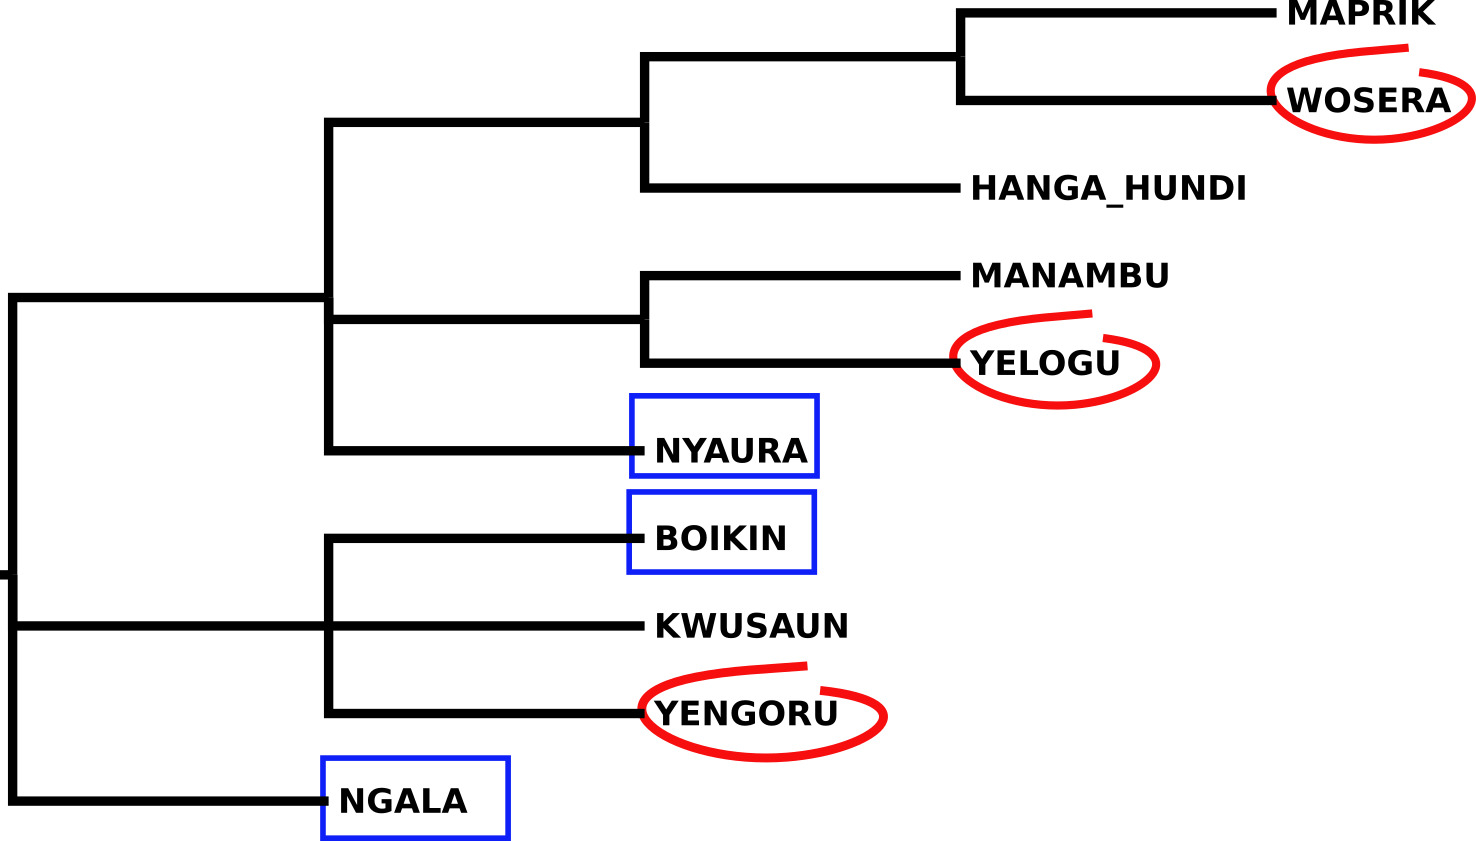
\includegraphics[width=5.20833in,height=2.96875in]{images//Ndu.glot_triplets.jpg}}

{In the midpoint rooted tree, the grouping is (Wosera, (Yelogu,
Yengoru)).}

{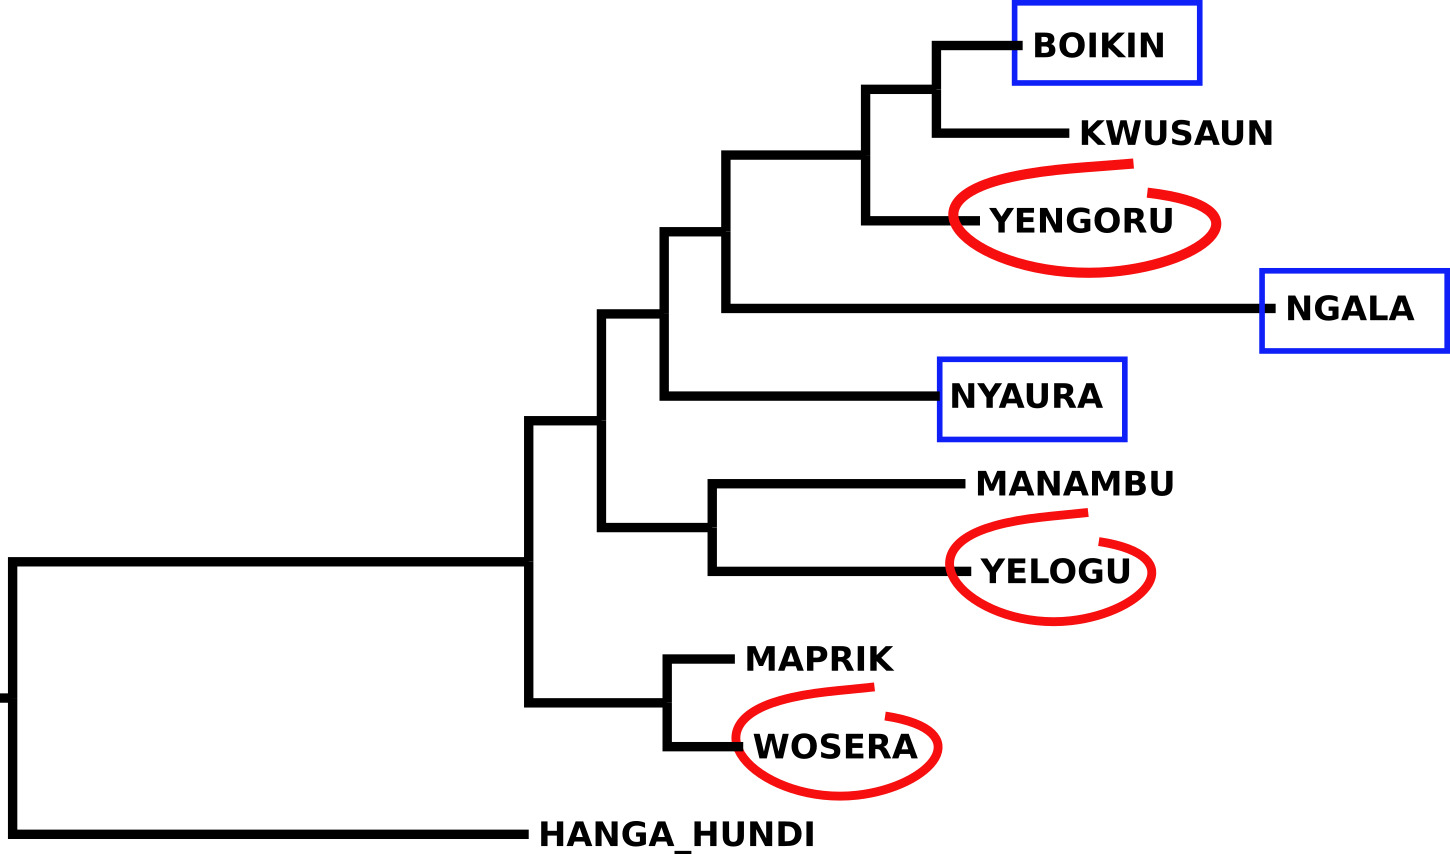
\includegraphics[width=5.27083in,height=3.10417in]{images/Ndu.midpointRooted.triplets.jpg}}

{So this triplet is mis-classified by midpoint rooting. This evaluation
is performed for each triplet of doculects. We disregard triplets like
(Ngala, Boikin, Nyaura), which remain unresolved in the goldstandard. I
call the number of misclassified triplets, divided by the number of
goldstandard-resolved triplets, the \emph{Generalized Triplet Distance}
(GTD) between the rooted binary-branching tree and the goldstandard
tree. (This is inspired by the \emph{Generalized Quartet Distance} from
Pompei et al.~2011).}

{I compared four rooting methods:}

\begin{enumerate}
\def\labelenumi{\arabic{enumi}.}
\item
  {\textbf{MAD rooting.}}
\item
  {\textbf{Midpoint rooting.}}
\item
  {\textbf{Outgroup rooting.} For this I created an artificial outgroup,
  with a character vector consisting entirely of 0s.}
\item
  {\textbf{Yule rooting.} This method is derived from (Steel and
  McKenzie 2001). They give a formula to compute the likelihood of a
  rooted tree \emph{topology} under the assumption that it was generated
  by a Yule process. The tree is rooted by calculating this likelihood
  for each possible root location and picking the one with the maximal
  likelihood. If there was a tie between different branches, I picked
  one at random.}
\end{enumerate}

{Here is the MAD rooted tree for Ndu (which happens to be identical to
the midpoint rooted version here):}

{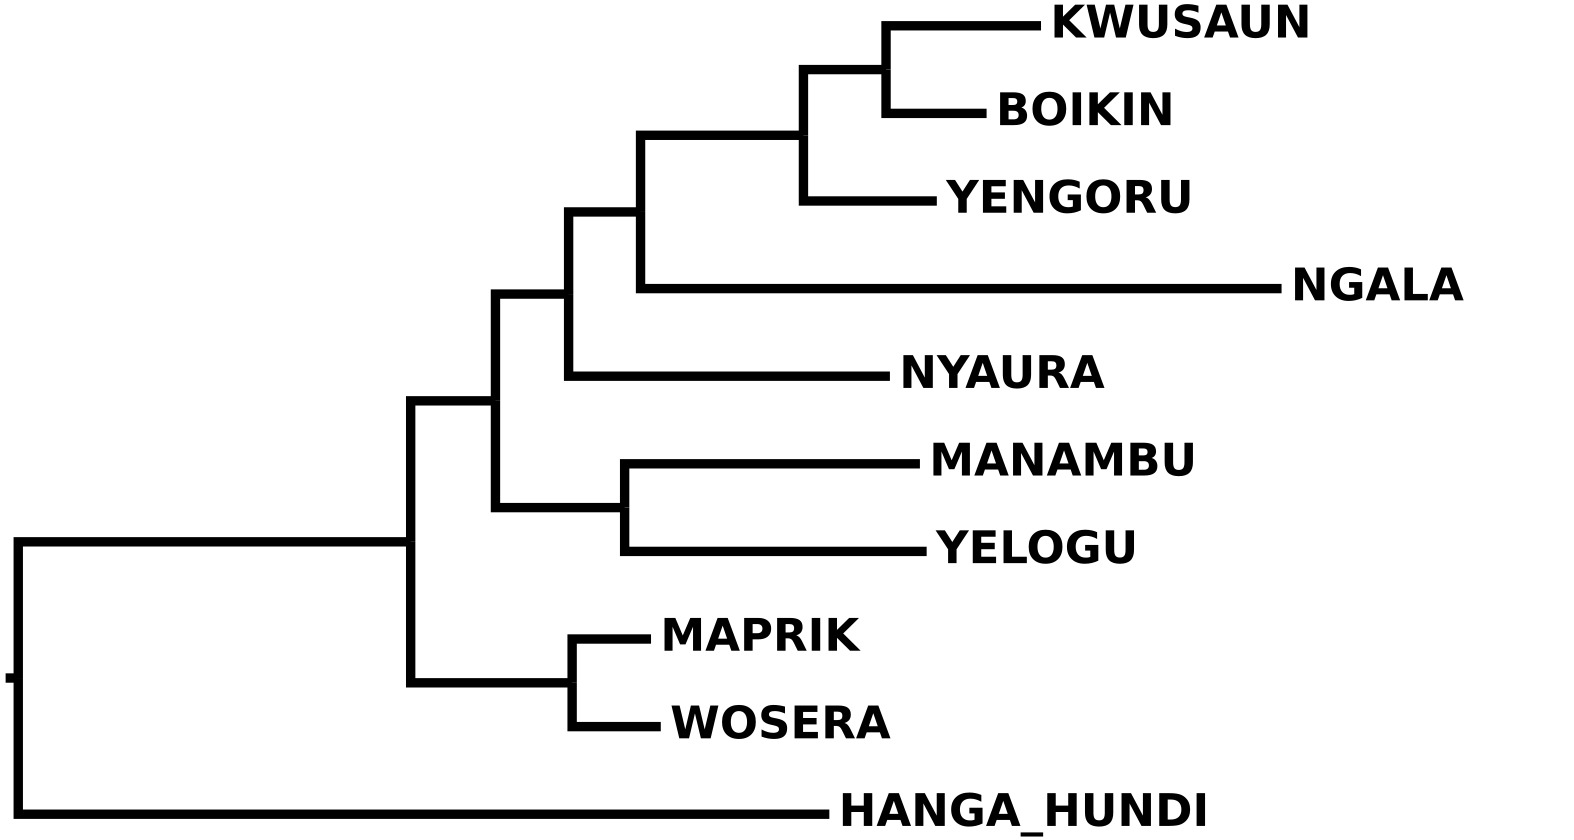
\includegraphics[width=5.21875in,height=2.78125in]{images/Ndu.madRooted.jpg}}

{The outgroup-rooted tree:}

{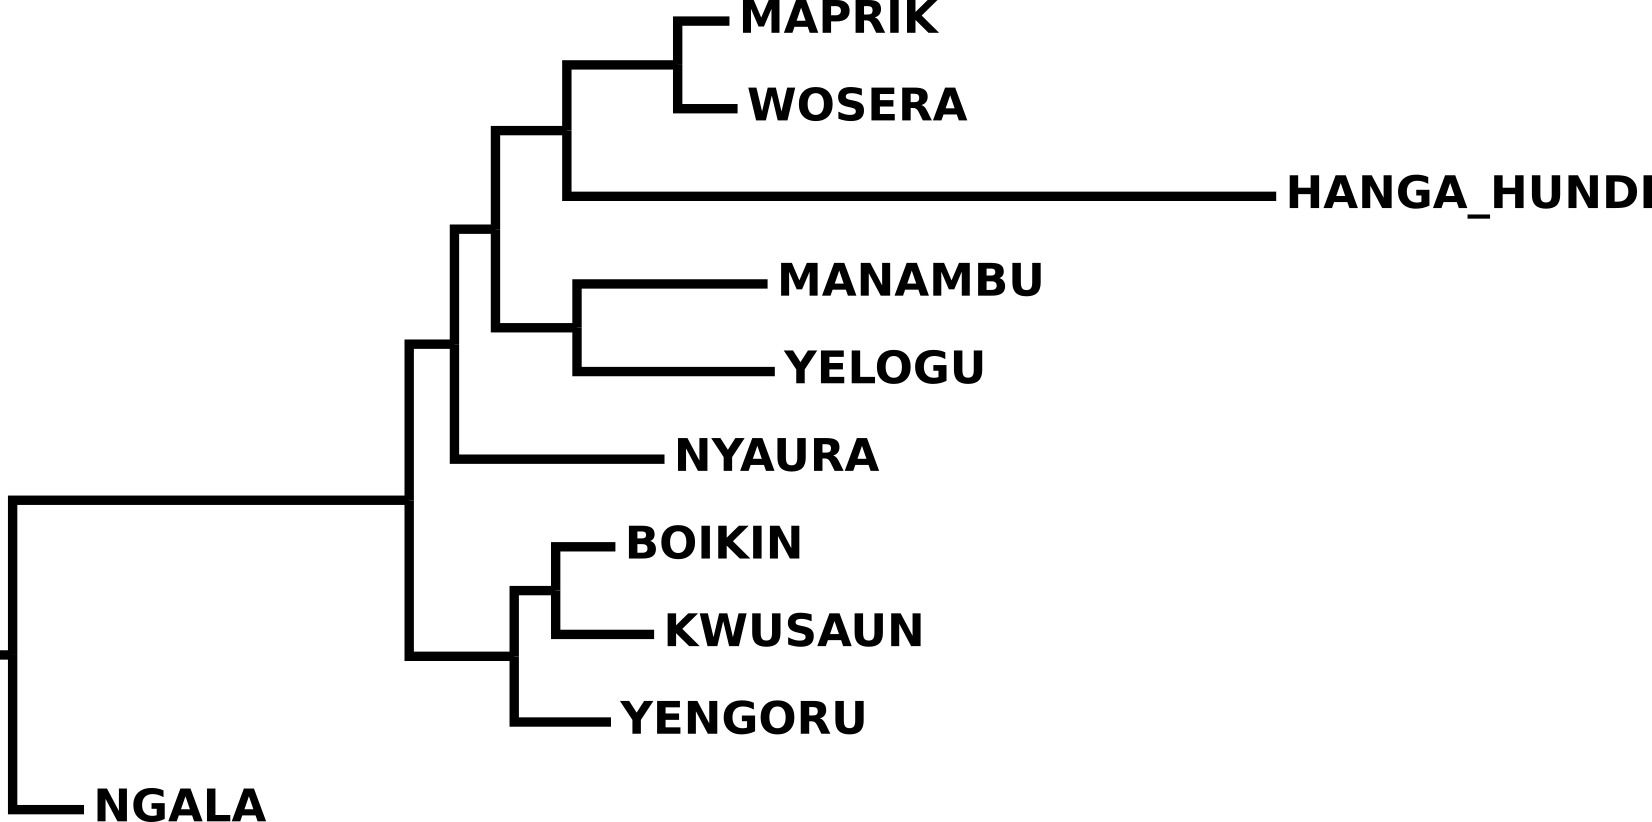
\includegraphics[width=5.20833in,height=2.59375in]{images/Ndu.outgroupRooted.jpg}}

{And the Yule-rooted version:}

{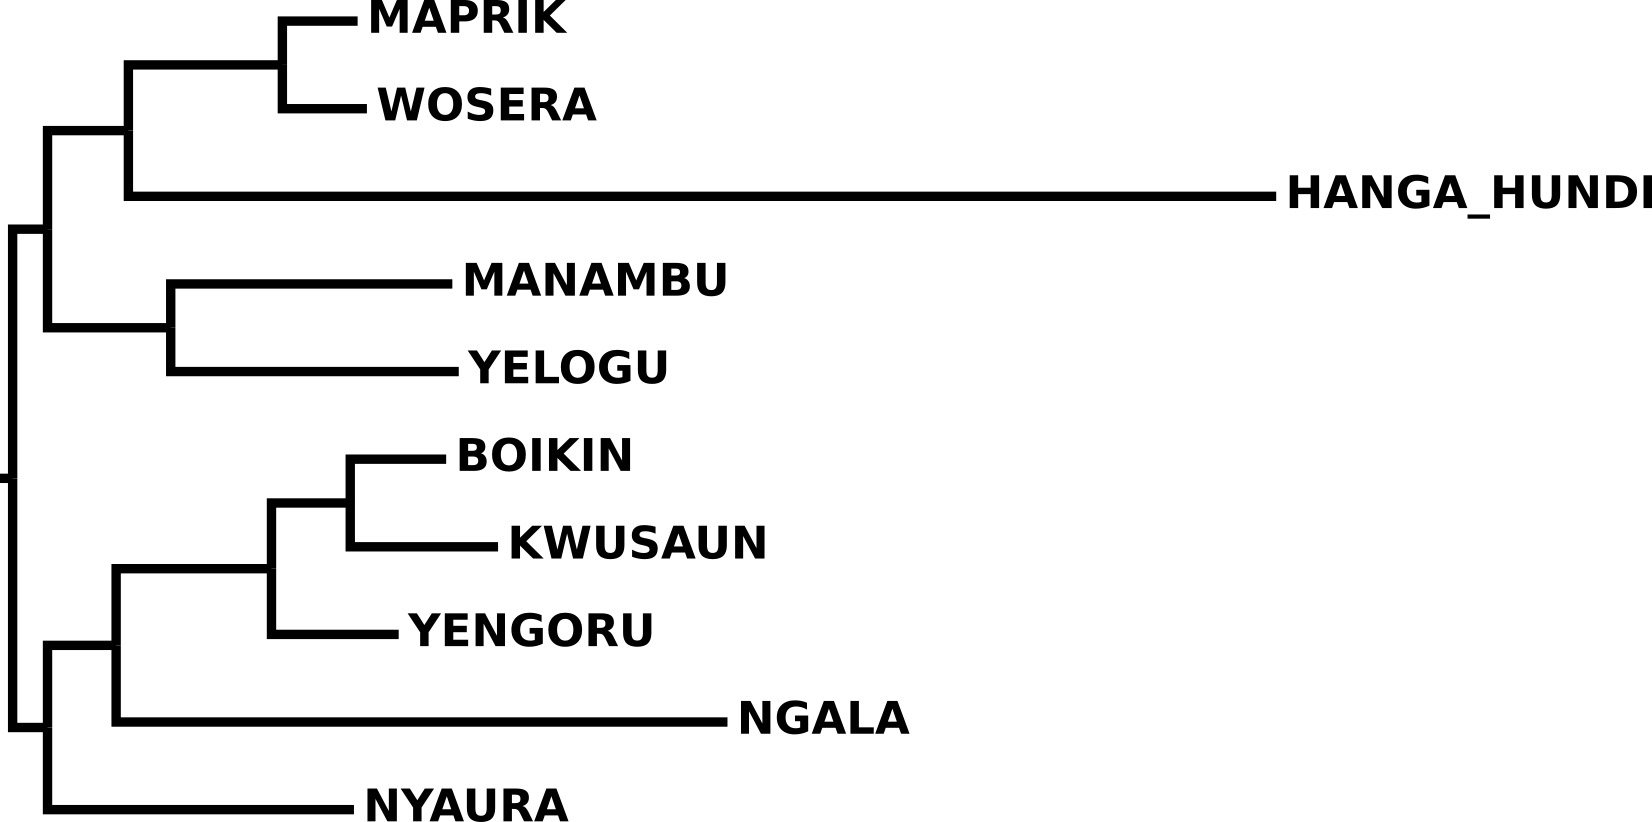
\includegraphics[width=5.22917in,height=2.60417in]{images/Ndu.yuleRooted.jpg}}

{Outgroup rooting is the only method here that produces a tree
consistent with the goldstandard. The GTDs are}

\begin{enumerate}
\def\labelenumi{\arabic{enumi}.}
\item
  {MAD: 0.61}
\item
  {midpoint: 061}
\item
  {outgroup: 0.00}
\item
  {Yule: 0.21}
\end{enumerate}

{It seems that both MAD and midpoint rooting are thrown off-stride here
by the extra-long branch extending to Hanga Hundi.}

{When we perform this comparison over all 64 families, we get a
different picture though:}

\begin{longtable}[]{@{}ll@{}}
\toprule
& {mean GTD}\tabularnewline
\midrule
\endhead
{\emph{MAD}} & {0.0704}\tabularnewline
{\emph{midpoint}} & {0.0941}\tabularnewline
{\emph{outgroup}} & {0.1437}\tabularnewline
{\emph{Yule}} & {0.1771}\tabularnewline
\bottomrule
\end{longtable}

{These numbers indicate quite clearly that MAD and midpoint rooting are
superior to both outgroup and Yule rooting. The difference between MAD
and midpoint rooting seems to be small, but closer examination reveals
that MAD is in fact substantially better than midpoint rooting.} - {MAD
rooting achieved a GTD of 0.0 (meaning: finds a root fully consistent
with the goldstandard) for 42 families (66\%), but midpoint rooting only
for 35 families (55\%).}- {Both MAD and midpoints rooting have a median
of 0, but the 75th quantile for MAD is at 0.10, and for midpoint at
0.16).}

{The difference is also clearly visible in the boxplots:}

{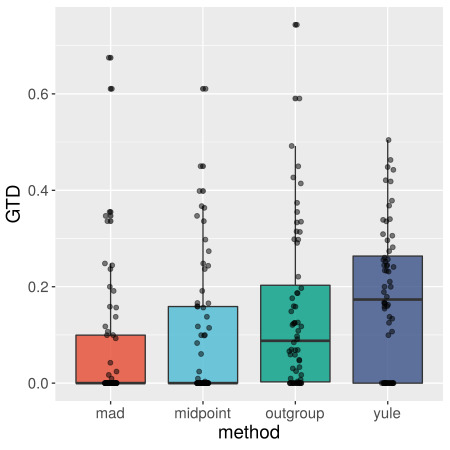
\includegraphics[width=4.75in,height=4.75in]{images/boxplots.jpg}}

{To conclude, \emph{Minimal Ancestor Deviation} rooting seems to be
better suited to root language phylogenies than more established
methods. The usual disclaimers apply -- we cannot be sure how much of
these results depend on the particular data and phylogenetic inference
method I used here. Different data might produce different results.
Still, MAD rooting deserves to be included into the standard toolbox of
phylogenetic linguistics.}

{Code and data, including all trees and the complete evaluation results,
are available at
\url{https://github.com/gerhardJaeger/competititiveRooting.git} .}

\subsection*{References}

\nopagebreak\hangindent=0.7cm {\small Jäger, G. (2018): Global-scale phylogenetic linguistic inference
from lexical resources, Scientific Data 5, 180189. URL:
https://doi.org/10.1038/sdata.2018.189 }

\nopagebreak\hangindent=0.7cm {\small Kümmel Tria, F. D., Landan, G., and T. Dagan (2017): Phylogenetic
rooting using minimal ancestor deviation. Nature Ecology and Evolution.
URL: http://dx.doi.org/10.1038/s41559-017-0193 }

\nopagebreak\hangindent=0.7cm {\small Pompei, S., Loreto, V., \& Kümmel Tria, F. D. (2011): On the
accuracy of language trees. \emph{PloS one} , \emph{6} (6), e20109. }

\nopagebreak\hangindent=0.7cm {\small Steel, M., \& McKenzie, A. (2001): Properties of phylogenetic trees
generated by Yule-type speciation models. \emph{Mathematical
biosciences} , \emph{170} (1), 91-112. }

\nopagebreak\hangindent=0.7cm {\small Sand et al.~(2014): tqDist: a library for computing the quartet and
triplet distances between binary or general trees, Bioinformatics,
30.14, 2079--2080. }

\nopagebreak\hangindent=0.7cm {\small Wichmann, Søren, Eric W. Holman, and Cecil H. Brown, eds., 2016. The
ASJP Database, version 17. URL: https://asjp.clld.org }

\vskip 2em
\framebox{\tabular{p{0.95\textwidth}}\textbf{Cite this article as}:
Gerhard J\"{a}ger,
\enquote{Rooting MADness,}
in \emph{Computer-Assisted Language Comparison in Practice},
22/05/2019,
\url{https://calc.hypotheses.org/1899}.\endtabular}


\newpage
\section*{Behind the Sino-Tibetan Database of Lexical
Cognates: Concept selection}
\phantomsection\addcontentsline{toc}{section}{Behind the Sino-Tibetan Database of Lexical
Cognates: Concept selection (Johann-Mattis List)}

Johann-Mattis List (26/06/2019)

\emph{Categories}: Primer

\emph{Tags}: code example, concept list, Concepticon, database,
Sino-Tibetan

\begin{center}\rule{0.5\linewidth}{1pt}\end{center}

One of the crucial steps in creating a database of lexical cognates is
the selection of concepts one wants to use for a given study. While many
scholars use the classical
\href{https://concepticon.clld.org/contributions/Swadesh-1952-200}{Swadesh
list of 200 items} ) (
\href{http://bibliography.lingpy.org?key=Swadesh1952}{Swadesh 1952} )
for this purpose, or the combined
\href{https://concepticon.clld.org/contributions/Comrie-1977-207}{list
of 207 items} , in which the former has been merged with Swadesh's
updated list of
\href{https://concepticon.clld.org/paramters/Swadesh-1955-100}{100
items} ( \href{http://bibliography.lingpy.org?key=Swadesh1955}{Swadesh
1955} ), and which is often mistakenly attributed to Swadesh himself,
although the first official reference seems to be
\href{http://bibliography.lingpy.org?key=Comrie1977}{Comrie (1977)} , it
is useful to give the selection of concepts some more thought initially.

What scholars underestimate usually in this context is that there are
quite different reasons why the classical Swadesh lists, or any
pre-compiled concept lists, may not be apt for the investigation of a
given language family. Apart from the obvious reason that a concept list
may contain terms that cannot be found in the target languages,
additional problems resulting from concept choice result from
language-specific characteristics of lexical typology, such as: (A)
sound symbolism, which may differ across languages, (B) compoundhood,
which also shows language-specific patterns, (C) polysemy or homophony,
which both may show areal or family-specific aspects.

In addition, one should not underestimate the importance of data
availability. Given that the majority of lexical databases are not
compiled from scratch, but derived from existing data collections which
serve as some kind of the backbone of the database, one should make sure
to check which concepts have been recorded in the major sources upon
which one wants to base the database.

When compiling the
\href{https://dighl.github.io/sinotibetan}{Sino-Tibetan Database of
Lexical Cognates} for our study on the origin of Sino-Tibetan (
\href{http://bibliography.lingpy.org?key=Sagart2019}{Sagart et al. 2019}
, we had to struggle with all of the above-mentioned points. Since our
initial goal was to create a database of \emph{high mutual coverage} in
terms of attested words per language (see
\href{http://bibliography.lingpy.org?key=List2018d}{List et al. 2018}
for a discussion of this concept), we had to pay specific attention to
the problem of data availability. For this reason, we started from an
initial comparison of concepts available different sources (including
those digitized by the STEDT project,
\href{http://bibliography.lingpy.org?key=Matisoff2015}{Matisoff 2015} ).
To compare the concepts available in the different sources, we made use
of the Concepticon project (
\href{https://concepticon.clld.org}{concepticon.clld.org} ,
\href{http://bibliography.lingpy.org?key=List2016a}{List et al. 2016} ,
see \href{http://bibliography.lingpy.org?key=List2018h}{List 2018} for
an introduction to the goals of the project) and the
\passthrough{\lstinline!pyconcepticon!} library, which offers quick
access to the resources offered by Concepticon.

When having installed the \passthrough{\lstinline!pyconcepticon!}
package, following the instructions provided at the project's
\href{https://github.com/concepticon/pyconcepticon/}{GitHub repository}
, one can easily check the overlap between several concept lists using
the \passthrough{\lstinline!intersection!} command that can be invoked
from the terminal (you have to replace \passthrough{\lstinline!PATH!}
with the path to your local Concepticon repository):

\begin{lstlisting}
$ concepticon --repos=PATH intersection Yakhontov-1991-35 Swadesh-1952-200 Swadesh-1955-100 Dolgopolsky-1964-15
1 EYE [1248]
2 I [1209]
3 LOUSE [1392]
4 NAME [1405]
5 THOU [1215]
6 TONGUE [1205]
7 TOOTH [1380]
8 TWO [1498]
9 WATER [948]
\end{lstlisting}

This code example checks which of the concepts given in the concept
lists by Swadesh (100 and 200) plus the lists by
\href{https://concepticon.clld.org/contributions/Yakhontov-1991-35}{Yakhontov}
(published in {[}Starostin 1991{]}) and
\href{https://concepticon.clld.org/contributions/Dolgopolsky-1964-15}{Dolgopolsky}
( \href{http://bibliography.lingpy.org?key=Dolgopolsky1964}{1964} )
recur in all lists, and outputs them both with their Concepticon Gloss,
and their Concepticon IDs. Note that you do not need to use the lists
that are provided by Concepticon alone, you can also compare with your
own concept lists, and this is exactly what we did, as we wanted to work
with data that was not yet officially linked to Concepticon (see the
\href{https://github.com/digling/edictor-tutorial}{tutorial} by
\href{http://bibliography.lingpy.org?key=List2017LECTUREd}{List 2017}
for more information).

While our first concept list consisted of as many as 250 concepts, we
had to reduce it further, once we started to add more languages to our
sample. Often, we ran into simple coverage problems, as some of the
concepts we thought would be useful turned out to be missing from
sources, and other concepts, like, e.g.,
\href{https://concepticon.clld.org/parameters/1509}{MOSQUITO} , were not
lexified in some regions of the Himalaya.

As a result, our final \enquote{master list}, which we used for the
phylogenetic analyses, only comprises 180 concepts. The criteria for
exclusion of concepts was strictly technical. We ranked all concepts by
their coverage with respect to the languages in our sample, and set up a
coverage of at least 80\% (each concept should be reflected in at least
80\% of our languages). We further removed some remaining concepts from
the list which had been shown to be problematic with respect to
compoundhood, sound symbolism, and polysemy.

Using Concepticon to check for coverage and overlap across concept lists
turned out to be very efficient, as it helped us to avoid to include
data into our database which did not provide enough coverage. To
illustrate how this can be done, we can compare the coverage of our
current list of 250 concepts in the database with the coverage of a
resource that we might want to add to our database in the future. This
resource is the database of cognates in Kho-Bwa languages, compiled by
T. A. Bodt (available from
\href{http://bibliography.lingpy.org?key=Bodt2019}{Bodt and List 2019}
). As Bodt's data and our data are linked to Concepticon (following the
recommendations of the \href{https://cldf.clld.org}{CLDF} initiative,
\href{http://bibliography.lingpy.org?key=Forkel2018a}{Forkel et al.
2018} ), we can compare their intersection with a simple command from
the terminal, in which we combine the original
\passthrough{\lstinline!intersection!} command of
\passthrough{\lstinline!pyconcepticon!} with the
\passthrough{\lstinline!wc!} command shipped with all Unix terminals by
using the famous and incredibly useful \passthrough{\lstinline!pipe!}
\passthrough{\lstinline!|!} :

\begin{lstlisting}
$ concepticon --repos=PATH intersection Sagart-2018-250.tsv Bodt-2019-664.tsv | wc -l
202
\end{lstlisting}

To run this code as illustrated here, the concept lists need to show a
certain format. You can check this out yourself by installing
\passthrough{\lstinline!pyconcepticon!} , downloading the Concepticon
data, and the two concept lists, which I have all uploaded to
\href{https://gist.github.com/LinguList/fa93b0829fede0d6cbb01f4ca5f5b864}{this
GitHub Gist}.

\subsection*{References}

\nopagebreak\hangindent=0.7cm {\small Bodt, Timotheus A. and List, Johann-Mattis (2019): Testing the
predictive strength of the comparative method: An ongoing experiment on
unattested words in Western Kho-Bwa langauges. Papers in Historical
Phonology 4.1. 22-44. }

\nopagebreak\hangindent=0.7cm {\small Comrie, Bernard and Smith, Norval (1977): Lingua Descriptive Series:
Questionnaire. Lingua 42. 1-72. }

\nopagebreak\hangindent=0.7cm {\small Dolgopolsky, Aron B. (1964): Gipoteza drevnejšego rodstva jazykovych
semej Severnoj Evrazii s verojatnostej točky zrenija {[}A probabilistic
hypothesis concering the oldest relationships among the language
families of Northern Eurasia{]}. Voprosy Jazykoznanija 2. 53-63. }

\nopagebreak\hangindent=0.7cm {\small Forkel, Robert and List, Johann-Mattis and Greenhill, Simon J. and
Rzymski, Christoph and Bank, Sebastian and Cysouw, Michael and
Hammarström, Harald and Haspelmath, Martin and Kaiping, Gereon A. and
Gray, Russell D. (2018): Cross-Linguistic Data Formats, advancing data
sharing and re-use in comparative linguistics. Scientific Data 5.180205.
1-10. }

\nopagebreak\hangindent=0.7cm {\small List, Johann-Mattis and Cysouw, Michael and Forkel, Robert (2016):
Concepticon. A resource for the linking of concept lists. In:
Proceedings of the Tenth International Conference on Language Resources
and Evaluation. 2393-2400. }

\nopagebreak\hangindent=0.7cm {\small List, Johann-Mattis (2017): Historical Language Comparison with
LingPy and EDICTOR {[}Historischer Sprachvergleich mit LingPy und
EDICTOR{]}. Department of Linguistic and Cultural Evolution: Max-Planck
Institute for the Science of Human History. }

\nopagebreak\hangindent=0.7cm {\small List, Johann-Mattis and Walworth, Mary and Greenhill, Simon J. and
Tresoldi, Tiago and Forkel, Robert (2018): Sequence comparison in
computational historical linguistics. Journal of Language Evolution 3.2.
130--144. }

\nopagebreak\hangindent=0.7cm {\small List, Johann-Mattis (2018): Towards a history of concept list
compilation in historical linguistics. History and Philosophy of the
Language Sciences 5.10. 1-14. }

\nopagebreak\hangindent=0.7cm {\small Matisoff, James A. (2015): The Sino-Tibetan Etymological Dictionary
and Thesaurus project. Berkeley:University of California. }

\nopagebreak\hangindent=0.7cm {\small Sagart, Laurent and Jacques, Guillaume and Lai, Yunfan and Ryder,
Robin and Thouzeau, Valentin and Greenhill, Simon J. and List,
Johann-Mattis (2019): Dated language phylogenies shed light on the
ancestry of Sino-Tibetan. Proceedings of the National Academy of Science
of the United States of America 116. 10317--10322. DOI:
\href{https://doi.org/10.1073/pnas.1817972116}{10.1073/pnas.1817972116} }

\nopagebreak\hangindent=0.7cm {\small Swadesh, Morris (1952): Lexico-statistic dating of prehistoric
ethnic contacts. With special reference to North American Indians and
Eskimos. Proceedings of the American Philosophical Society 96.4.
452-463. }

\nopagebreak\hangindent=0.7cm {\small Swadesh, Morris (1955): Towards greater accuracy in lexicostatistic
dating. International Journal of American Linguistics 21.2. 121-137. }

\vskip 2em
\framebox{\tabular{p{0.95\textwidth}}\textbf{Cite this article as}:
Johann-Mattis List,
\enquote{Behind the
Sino-Tibetan Database of Lexical Cognates: Concept selection,}
in \emph{Computer-Assisted Language Comparison in Practice},
26/06/2019,
\url{https://calc.hypotheses.org/1933}.\endtabular}


\newpage
\section*{Using the Waterman-Eggert algorithm for
sentence alignment}
\phantomsection\addcontentsline{toc}{section}{Using the Waterman-Eggert algorithm for
sentence alignment (Johann-Mattis List)}

Johann-Mattis List (15/07/2019)

\emph{Categories}: Code

\emph{Tags}: code snippet, sentence alignment, sequence alignment,
Waterman-Eggert algorithm

\begin{center}\rule{0.5\linewidth}{1pt}\end{center}

During the 24th International Conference of Historical Linguistics, I
was asked by a colleague whether I would know a good way to align and
scores sentences available in form of phonetic transcriptions. While it
is clear that one can roughly compare the difference between sequences
rather easily by aligning them, and calculating, for example, the edit
distance between them, it is clear that the task of sentence alignment
could be done in a somewhat more subtle way.

The first obstacle that we may meet when trying to align sentences is
that a completely linear alignment may yield problems, since sentences
may contain the same or similar words, but differ with respect to word
order. The first alignment algorithm that comes to mind when trying to
deal with this question is the so-called
\href{http://www.bioinformatics.nl/cgi-bin/emboss/help/matcher}{Waterman-Eggert
algorithm} , first proposed and named after
\href{http://bibliography.lingpy.org?key=Waterman1987}{Waterman and
Eggert (1987)} .

Long time ago, I provided an implementation of this algorithm as part of
the LingPy package. The basic idea compared to traditional alignment
algorithms is to expand upon local alignment when searching for optimal
subsequences between two strings. While local alignment stops after
having identified the longest similar subsequence between two strings,
the Waterman-Eggert algorithm does not stop, but instead continuous
searching for more similar subsequences in the data, just until all of
them have been readily identified.

This is not the place to get into the details of the algorithmics here.
For those interested in the topic, I recommend to have a look at
\href{http://bibliography.lingpy.org?key=List2014d}{List (2014)} , where
the major algorithms for alignment analyses have been rdescribed and
discussed for usability in linguistic applications. To get a sbrief
glimpse at the crucial difference between Waterman-Eggert and the famous
local alignment algorithm by Smith-Waterman (
\href{http://bibliography.lingpy.org?key=Smith1981}{Smith and Waterman
1981} ), let us open a terminal and test the Waterman-Eggert algorithm
in a short \href{http://lingpy.org}{LingPy} session (
\href{http://bibliography.lingpy.org?key=List2018i}{List et al. 2018} ).

\begin{lstlisting}
>>> from lingpy import *
>>> for a, b, c in we_align('abcd', 'cdab'):
...     print(' '.join(a))
...     print(' '.join(b))
...     print('-')
a b
a b
-
c d
c d
\end{lstlisting}

What should be clear from this illustration is that the algorithm does
not simply align strings locally, but instead that it searches for
substring matches. This is internally done by identifying the
highest-scoring subsequence in the alignment matrix at first, and then
searching again for the next-high-scoring subsequence, until none are
left.

To use this for sentence alignment of sentences provided in phonetic
transcription, we can write a wrapper function that makes use the
Waterman-Eggert implementation given in LingPy. In addition to simply
aligning two sentences, however, we would also like to score them, and
we will soon see how this can be done. We first start by loading a patch
for the Waterman-Eggert algorithm, since I realized that the current
LingPy implementation contains a bug. This patch is provided along with
the code in a
\href{https://gist.github.com/LinguList/8189f06f231909fbf1d1eed30998bd83}{GitHub-Gist}
accompanying this post.

We start our script by loading the libraries. Here, we load LingPy, the
patch (which will soon be included when we do the next update), and the
\passthrough{\lstinline!product!} function from itertools, which we need
to populate our scoring dictionary.

\begin{lstlisting}
from lingpy import *
from patch_we_align import we_align
from itertools import product
\end{lstlisting}

We now start by defining our function. It has a rather simple call
signature with a few parameters. The first parameters are the sentences,
which should be given in IPA transcription without any punctuation
marks. The gap penalty is the classical gap penalty passed to the
alignment algorithm. The model refers to the sound class model, i.e., it
determines how we represent sounds internally in our function. The
default is the \passthrough{\lstinline!sca!} model also widely used in
LingPy. The limit-argument tells the function which subsequences it
should still accept as matches. I think, for initial tests, subsequences
of length two seem like a good start here.

\begin{lstlisting}
def salign(
        senA,
        senB,
        gap=-1,
        model='sca',
        limit=2
        ):
    """Align and score two sentences"""
\end{lstlisting}

In the next step, we convert the sentences into sound classes, using the
sound class model. To do so, we first tokenize them, i.e., we determine
what should count as a sound. This function will treat combinations of
base-letters and diacritics as one sound. If you do not want to use it,
just provide your data already in space-segmented form, and this
function won't do anything. We then convert the segmented data (a Python
list as data type) into sound class representations.

\begin{lstlisting}
    # retrieve sound class model
    if not hasattr('scorer', model):
        model = Model(model)
    # convert to sound classes
    tokA, tokB = list(map(
        lambda x: ipa2tokens(
            x.replace(' ', '_')),
        [senA, senB]))

    # assume segmentation by underscore
    clsA, clsB = list(map(
        lambda x: tokens2class(
            x,
            model
            ),
        [tokA, tokB]
        ))
\end{lstlisting}

Before we can now align the data with the Waterman-Eggert algorithm, we
need to create a scorer that tells the algorithm how segments should be
compared with each other. Here, we simply use the built-in scorer
provided along with the LingPy package, setting the matching of
\passthrough{\lstinline!\_!} with itself to \passthrough{\lstinline!0!}
, because we do not want to enourage the algorithm to align too many
boundary markers with each other.

\begin{lstlisting}
    scorer = {(a, b): -1 if \
            (a != b or '_' in (a, b)) \
            else 1 for a, b in product(
            set(clsA+clsB),
            set(clsA+clsB))
        }
    # make sure boundaries don't score
    scorer['_', '_'] = 0
\end{lstlisting}

We can now start to compute the alignments. While doing so, we iterate
over each identified segment and store their similarity in a specific
list, so we can later used it for scoring the similarity of the
sentences. Our patch has the advantage of offering a detailed index of
which elements have been aligned (different from the original call
signature). We use this to extract the original transcriptions as
alignments, rather than the aligned sound classes.

\begin{lstlisting}
    out, scores = [], []
    for a, b, score, iA, iB in we_align(
        clsA, clsB, scorer=scorer, gap=gap
        ):
        if len(a) < limit:
            pass
        else:
            out += [
                    (a, b, score)
                    ]
            scores += [score]
\end{lstlisting}

While we could already output the data as is, it would be useful to
score the data as well, in order to offer us a way to retrieve some
general distance between the two sentences. In order to do so, we just
follow \href{http://bibliography.lingpy.org?key=Downey2008}{Downey et
al. (2008)} in computing a normalized distance score from the similarity
scores that we retrieve for each aligned subsequence in comparison with
the alignments of each sentence with itself.

\begin{lstlisting}
    # compute self-scores
    sA = sum([scorer[a, a] for a in clsA])
    sB = sum([scorer[a, a] for a in clsB])
    sAB = sum(scores) / len(scores)

    score = 1 - (2 * sAB / (sA + sB))
    return out, score
\end{lstlisting}

Equipped with this code, we can now carry out our first sentence
alignment. Let's compare two random sentences from German with each
other in which we deliberately re-arrange some words.

\begin{lstlisting}
alms, scores = salign(
        'mainəʁuː.ɪsthɪnsainhɛrt͡s',
        'hɛrt͡smainʁuː.əsain',
        gap=-2
        )
for a, b, score in alms:
    print(' '.join(a))
    print(' '.join(b))
    print('{0:.2f}'.format(score))
print('{0:.2f}'.format(scores))
\end{lstlisting}

The output of this comparison (the first sentence is inspired by
Goethe's \enquote{Meine Ruh' ist hin}) yields the following results:

\begin{lstlisting}
H E R C
H E R C
4.00
S A N
S A N
3.00
M A N E R Y
M A N - R Y
3.00
0.38
\end{lstlisting}

In total, the algorithm yields three blocks, which correspond to four
words in the original data, with the third block (corresponding to
\enquote{meine Ruh}) showing the same order in both test sequences. The
last score, 0.38, is the overall distance of the two sequences, which is
rather low, given the high number of words occuring in the sequence.

It is clear that more can be done to arrive at a good sentence
alignment. This post was not meant to present a complete solution to the
problem, it was rather intended to illustrate how we can use the tools
we offer in libraries such as LingPy to carry out quick tests on new
topics that have so far not yet been thoroughly discussed in the field
of comparative linguistics. Code and patch are available in form of a
GitHub Gist, which you can download from
\href{https://gist.github.com/LinguList/8189f06f231909fbf1d1eed30998bd83}{here}.

\subsection*{References}

\nopagebreak\hangindent=0.7cm {\small Downey, Sean S. and Hallmark, Brian and Cox, Murray P. and Norquest,
Peter and Lansing, Stephen (2008): Computational feature-sensitive
reconstruction of language relationships: developing the ALINE distance
for comparative historical linguistic reconstruction. \emph{Journal of
Quantitative Linguistics} 15.4. 340-369. }

\nopagebreak\hangindent=0.7cm {\small List, Johann-Mattis (2014): Sequence comparison in historical
linguistics. Düsseldorf:Düsseldorf University Press. }

\nopagebreak\hangindent=0.7cm {\small List, Johann-Mattis and Greenhill, Simon and Tresoldi, Tiago and
Forkel, Robert (2018): LingPy. A Python library for quantitative tasks
in historical linguistics. Max Planck Institute for the Science of Human
History. Jena: \href{//lingpy.org”}{http://lingpy.org} . }

\nopagebreak\hangindent=0.7cm {\small Smith, T. F. and Waterman, M. S. (1981): Identification of common
molecular subsequences. \emph{Journal of Molecular Biology} 1.
195-197. }

\nopagebreak\hangindent=0.7cm {\small Waterman, M. S. and Eggert, M. (1987): A new algorithm for best
subsequence alignments with application to tRNA-rRNA comparisons.
\emph{Journal of Molecular Biology} 197. 723-728. }

\vskip 2em
\framebox{\tabular{p{0.95\textwidth}}\textbf{Cite this article as}:
Johann-Mattis List,
\enquote{Using the
Waterman-Eggert algorithm for sentence alignment,}
in \emph{Computer-Assisted Language Comparison in Practice},
15/07/2019,
\url{https://calc.hypotheses.org/1941}.\endtabular}


\newpage
\section*{Feature-Based Alignment Analyses with
LingPy and CLTS (1)}
\phantomsection\addcontentsline{toc}{section}{Feature-Based Alignment Analyses with
LingPy and CLTS (1) (Johann-Mattis List)}

Johann-Mattis List (19/08/2019)

\emph{Categories}: Code

\emph{Tags}: alignment, cross-linguistic transcription systems,
distinctive features, phonetic alignment, Python, scoring function

\begin{center}\rule{0.5\linewidth}{1pt}\end{center}

In the past, people have repeatedly asked me how they could use their
own scoring functions in combination with LingPy's alignment algorithms.
Their major concern was that the sound-class-based scoring systems we
use in LingPy might fail to reflect true phonetic similarity of sounds,
specifically also because they are not informed by classical ideas about
distinctive features in phonology. As described in detail in
\href{http://bibliography.lingpy.org?key=List2014d}{List (2014)} ,
LingPy converts sounds in phonetic transcription to an internal alphabet
of less than 30 letters, to which the alignment algorithms are then
applied in a second stage.

What my colleagues wanted to do instead was to test feature-based
scoring systems
(e.g.~\href{http://bibliography.lingpy.org?key=Chomsky1968}{Chomsky and
Halle 1968} ) and then use these features to derive distance or
similarity scores between phonetic segments which would then be used to
carry out the alignment analysis. In addition, some colleagues had
created their own similarity matrix, and wanted to apply it more
flexibly to other datasets (see, for example,
\href{http://bibliography.lingpy.org?key=Jaeger2015}{Jäger 2015} ). My
answer was usually, that this could be done in principle, but that it
would require some amount of data preprocessing, depending on what data
one wants to align. Not many colleagues asked me a second time, maybe
because they thought it would be too complicated to use their own
distance or similarity scores in LingPy.

When I recently started working on a modified alignment algorithm
myself, I had to work on the same question again, and I figured, that it
is in fact not that difficult to use a custom scoring function in
Lingpy. Most of the things one needs to use LingPy along with custom
scoring functions are already in place. Furthermore, with our recently
published \href{https://github.com/cldf/clts}{pyclts} package,
underlying the \href{https://clts.clld.org}{Database of Cross-Linguistic
Transcription Systems} (see
\href{http://bibliography.lingpy.org?key=Anderson2018}{Anderson et al.
(2018)} for an overwiew), there is now even a large collection of sounds
for which we have distinctive feature sets. The major reason why I never
tested feature-based alignment methods so far, was that I could not find
a feature-system that would offer feature for all the sounds I usually
find in linguistic datasets. Even datasets like
\href{https://phoible.org}{Phoible} (
\href{http://bibliography.lingpy.org?key=Moran2014}{Moran et al. 2014}
), which offers huge amounts of transcriptions barely touch the surface
of the variation one encounters when working with real transcriptions.

Luckily, our CLTS system has shown to be very robust so far. It
understands some 8000 different phonetic segments, including clicks,
tones, dipththongs, and certain consonant clusters, and we have
developed first approaches to convert a given dataset into a form of IPA
that CLTS accepts. For the conversion, we now use \emph{orthography
profiles} ( \href{http://bibliography.lingpy.org?key=Moran2018}{Moran
and Cysouw 2018} ), which I have presented in past tutorials (
\href{http://bibliography.lingpy.org?key=List2017LECTUREd}{List 2017} ),
and for which I recently also wrote an implementation in JavaScript,
called \href{http://calc.digling.org/}{SegmentsJS} .

I therefore think that it is time to get back to my colleagues' request
and illustrate how one can first create a custom, feature-based scoring
function with help of CLTS, and then use this scoring function to carry
out pairwise alignments of phonetic sequences. Given my limited time to
write tutorial blogposts, I furthermore decided to divide this post into
two (potentially three) posts, and discuss the creation of the scoring
function in this post, while I will get back to the question of how to
use LingPy's methods for sequence comparison in one or two follow-up
posts.

Before we start with the actual code, it is important to understand how
scoring functions work. Basically there are two different kinds of
scoring functions: those based on \emph{distances} between segments, and
those based on \emph{similarities} between segments. One may intuitively
think that there is no real difference with respect to the use of
similarities or distances. When looking closer into the algorithmics
underlying the sequence alignment problem, however, this assumption is
not correct, since only similarity-based scoring functions allow for
both semi-global and local alignment analyses (for details on these
problems, compare
\href{http://bibliography.lingpy.org?key=List2014d}{List 2014} , where
all algorithms are described in detail).

For this reason, it is not useful to start from the computation distance
scores for phonetic segments. Instead, I recommend everybody who wishes
to work seriously on phonetic alignment algorithms to work with those
algorithms that make use of similarities between segments. While
distance scores are probably easy to understand, since we can think of
them in form of distance in space, or distance along pathways, or
distance in trees. Distance between identical objects is always 0, and
the more dissimilar two objcts become, the higher the distance score
between them. Similarity scores, on the other hand, assume some high
score for the identity of objects, which may vary, depending on the
object under question, and smaller scores for dissimilar objects, with
scores beyond zero being reserved for those objects that have almost
nothing in common.

In order to derive a \emph{distance score} between two sound segments
which are defined by a given feature system, the easiest and seemingly
most straightforward way (recommended and defended by some colleagues in
personal communication) is to compute the so-called \emph{Hamming
distance} (
\href{http://bibliography.lingpy.org?key=Hamming1950}{Hamming 1950} .
This distance reflects the proportion of features where two segments
differ. Turning the Hamming distance into a similarity score is
straightforward, since we only need to calculate the proportion of
features where two segments are identical.

If we look at the CLTS feature system, we find 37 features in total,
which cover three major classes of sounds, \emph{consonants} ,
\emph{vowels} , and \emph{tones} , which themselves may vary with
respect to the features that define them. The features themselves can be
binary or have multiple values. Retrieving the features of a given sound
linked to the CLTS system is straightforward. The features can be found
in the \passthrough{\lstinline!featuredict!} attribute of a
\passthrough{\lstinline!Sound!} object.

\begin{lstlisting}
from pyclts import TranscriptionSystem
bipa = TranscriptionSystem('bipa')
sound = bipa['ts']
for i, (k, v) in enumerate(sorted(sound.featuredict.items())):
    print('{0:5} | {1:22} | {2:10}'.format(i+1, k, v or '-'))
\end{lstlisting}

When you type in this code in your commandline (provided you have
installed the \href{https://pypi.org/project/pyclts/}{pyclts} package,
e.g., with help of \passthrough{\lstinline!pip!} , by typing
\passthrough{\lstinline!pip install pyclts!} ), you will receive the
output shown in the following table in text form.

\begin{longtable}[]{@{}lll@{}}
\toprule
No. & Feature & Value\tabularnewline
\midrule
\endhead
1 & articulation & --\tabularnewline
2 & aspiration & --\tabularnewline
3 & breathiness & --\tabularnewline
4 & creakiness & --\tabularnewline
5 & duration & --\tabularnewline
6 & ejection & --\tabularnewline
7 & glottalization & --\tabularnewline
8 & labialization & --\tabularnewline
9 & laminality & --\tabularnewline
10 & laterality & --\tabularnewline
11 & manner & affricate\tabularnewline
12 & nasalization & --\tabularnewline
13 & palatalization & --\tabularnewline
14 & pharyngealization & --\tabularnewline
15 & phonation & voiceless\tabularnewline
16 & place & alveolar\tabularnewline
17 & preceding & --\tabularnewline
18 & raising & --\tabularnewline
19 & relative \passthrough{\lstinline!\_!} articulation --
&\tabularnewline
20 & release & --\tabularnewline
21 & sibilancy & sibilant\tabularnewline
22 & syllabicity & --\tabularnewline
23 & velarization & --\tabularnewline
24 & voicing & --\tabularnewline
\bottomrule
\end{longtable}

We can see from the output that CLTS currently uses as many as 24
different features to define consonants, which mostly reflect the
traditional way in which sounds are defined by the International
Phonetic Alphabet (
\href{http://bibliography.lingpy.org?key=IPA1999}{IPA 1999} ). You can
apply the same procedure to check for the vowel and the tone features
applied by CLTS, by replacing the line
\lstinline!sound = bipa['ts']! by the line
\lstinline!sound = bipa['a']! or
\lstinline!sound = bipa['⁵⁵']! , respectively.

With our feature vector and a system like CLTS which offers feature
values, it is straightforward to write a short function that allows us
to compare the hamming distance between different sounds transcribed in
\emph{Broad IPA} ( \passthrough{\lstinline!bipa!} ) system offered by
the CLTS database.

We start by defining our function for scoring two sound segments. This
function accepts two paremeters (the sound segments, passed as strings),
and three keywords, \passthrough{\lstinline!bipa!} (referring to the
\passthrough{\lstinline!bipa!} transcription system offered by the
\passthrough{\lstinline!pyclts!} package),
\passthrough{\lstinline!classes!} (a function that defines to which
score we want to normalize our Hamming similarities), and
\passthrough{\lstinline!features!} , the list of feature vectors, as
offered per class in our transcription system.

\begin{lstlisting}
from pyclts.transcriptionsystem import TranscriptionSystem
from itertools import combinations

def score_sounds(
        a,
        b,
        features=None,
        classes=None,
        bipa=None
        ):
    """
    Score sounds with Hamming distance from feature system.
    """
    # load bipa object
    bipa = bipa or TranscriptionSystem('bipa')

    # define the features
    features = features or {
        "consonant": list(
            bipa['t'].featuredict),
        "vowel": list(
            bipa['a'].featuredict),
        "tone": list(
            bipa['⁵⁵'].featuredict)
        }
    # define base score for the classes
    classes = classes or {
        "consonant": 1,
        "vowel": 1,
        "tone": 1
        }
\end{lstlisting}

You can see from this first code block that I was lazy and did not spell
out the feature systems, but retrieved them from dummy sounds. As we
will see later, however, we will usually create our feature vectors
before and pass them to the method via the keywords, also to avoid that
the Broad IPA is loaded on every call, which will drastically influence
the performance of this method.

Our next step consists in the conversion of our sounds to our
\passthrough{\lstinline!TranscriptionSystem!} in CLTS, and to check for
dipthongs or clusters. Dipthongs and clusters are not defined by their
own features in CLTS, but rather have separate features for the first
and the second sound, which can be accessed through their attributes
\passthrough{\lstinline!from\_sound!} and
\passthrough{\lstinline!to\_sound!} . To keep the demonstration simple
for the time being, we will for now simply represent the complex sounds
by their first sound.

\begin{lstlisting}
    # convert sounds to transcription system
    sA, sB = bipa(a+' '+b)

    # check for diphthongs or clusters
    if hasattr(sA, 'from_sound'):
        sA = sA.from_sound
    if hasattr(sB, 'from_sound'):
        sB = sB.from_sound
\end{lstlisting}

Now we make sure to return a high negative value in those cases where
the base classes for all sounds in CLTS turn out to be different. This
score is in fact arbitrary, as long as it is low enough, since we want
to avoid no matter what, that alignments mix the sound classes (some
colleagues were not happy with this decision in the past, but my
experience clearly shows that not separating classes leads to an
unexpected alignment behavior that is extremely difficult to control).

\begin{lstlisting}
    # return -10 if classes don't match
    if sA.type != sB.type:
        return -10
\end{lstlisting}

Now, we are almost done with our function that calculates segment
similarities based on distinctive feature systems. In order to compute
the Hamming similarity, we first define the base similarity, which is
reflecting the size of the feature vector, and then calculate the factor
needed to normalize the data consistently. According to our defaults,
which we wrote into the function, the highest similarity score for all
sound classes is 1, so normalization will yield scores between 0 and 1
for our Hamming similarities.

\begin{lstlisting}
    # base score is the number of features
    sim = len(features[sA.type])

    # normalization factor
    normalize = classes[sA.type] / sim

    # return in case of identity
    if a == b:
        return sim * normalize

    # reduce similarity in case of mismatch
    for feature in features[sA.type]:
        if sA.featuredict[feature] != sB.featuredict[feature]:
            sim -= 1
    return sim * normalize
\end{lstlisting}

Now that we can compute our Hamming similarities, we can test this
function directly by feeding it different sounds. In order to get a
full-fledged scoring dictionary, however, which we will need to carry
out a phonetic alignment analysis, it is useful to write another
function that takes a couple of sounds as input and returns a scoring
dictionary in which all sounds are compared with each other. The
function takes a bunch of letters as parameter, and also the three
keywords, which we already defined for the
\passthrough{\lstinline!score\_sounds!} function.

\begin{lstlisting}
def get_scorer(
        letters,
        bipa=None,
        classes=None,
        features=None
        ):
    """
    Retrieve a scoring dictionary for alignment algorithms.
    """
    # load bipa object
    bipa = bipa or TranscriptionSystem('bipa')

    # define the features
    features = features or {
        "consonant": list(
            bipa['t'].featuredict),
        "vowel": list(
            bipa['a'].featuredict),
        "tone": list(
            bipa['⁵⁵'].featuredict)
        }
    # define base score for the classes
    classes = classes or {
        "consonant": 1,
        "vowel": 1,
        "tone": 1
        }
\end{lstlisting}

After this boring part, where we repeat the same code (this may
definitely be enhanced further, but for demonstration purposes, it is
surely enough), we can now compute the scorer. This can be done in a
very straightforward way with help of the
\passthrough{\lstinline!combinations!} method offered by the
\passthrough{\lstinline!itertools!} module, which is part of Python.

\begin{lstlisting}
    scorer = {}
    bipa = bipa or TranscriptionSystem('bipa')
    for a, b in combinations(letters, r=2):
        scorer[a, b] = scorer[b, a] = score_sounds(a, b, bipa=bipa)
        scorer[a, a] = score_sounds(a, a, bipa=bipa)
        scorer[b, b] = score_sounds(b, b, bipa=bipa)

    return scorer
\end{lstlisting}

Now, we can finally start and see, how well this approach works. For
convenience, I use the tabulate package for printing of tables, and
define a couple of sounds whose similarity I want to investigate.

\begin{lstlisting}
from tabulate import tabulate
cons = ['p', 't', 'b', 'd', 'pʰ', 'tʰ']
vows = ['a', 'e', 'i', 'o', 'u']
scorer = get_scorer(cons+vows)
\end{lstlisting}

When retrieving the similarity matrix from the scorer now, we can easily
construct a matrix, which illustrates the difference between the sounds
in our sample.

\begin{lstlisting}
matrix = [[1 for x in cons] for y in cons]
for (i, a), (j, b) in combinations(enumerate(cons), r=2):
    matrix[i][j] = matrix[j][i] = round(scorer[a, b], 2)
for i, (c, r) in enumerate(zip(cons, matrix)):
    matrix[i] = [c]+r
print(tabulate(matrix, headers=cons, tablefmt='pipe'))
\end{lstlisting}

The matrix for the consonants in our sample is shown in the following
table.

\begin{longtable}[]{@{}lrrrrrr@{}}
\toprule
\endhead
& \textbf{p} & \textbf{t} & \textbf{b} & \textbf{d} & \textbf{pʰ} &
\textbf{tʰ}\tabularnewline
\textbf{p} & 1 & 0.96 & 0.96 & 0.92 & 0.96 & 0.92\tabularnewline
\textbf{t} & 0.96 & 1 & 0.92 & 0.96 & 0.92 & 0.96\tabularnewline
\textbf{b} & 0.96 & 0.92 & 1 & 0.96 & 0.92 & 0.88\tabularnewline
\textbf{d} & 0.92 & 0.96 & 0.96 & 1 & 0.88 & 0.92\tabularnewline
\textbf{pʰ} & 0.96 & 0.92 & 0.92 & 0.88 & 1 & 0.96\tabularnewline
\textbf{tʰ} & 0.92 & 0.96 & 0.88 & 0.92 & 0.96 & 1\tabularnewline
\bottomrule
\end{longtable}

By replacing the \passthrough{\lstinline!cons!} variable by
\passthrough{\lstinline!vows!} , we can produce the same matrix for our
vowels.

\begin{longtable}[]{@{}lrrrrr@{}}
\toprule
\endhead
& \textbf{a} & \textbf{e} & \textbf{i} & \textbf{o} &
\textbf{u}\tabularnewline
\textbf{a} & 1 & 0.95 & 0.95 & 0.85 & 0.85\tabularnewline
\textbf{e} & 0.95 & 1 & 0.95 & 0.9 & 0.85\tabularnewline
\textbf{i} & 0.95 & 0.95 & 1 & 0.85 & 0.9\tabularnewline
\textbf{o} & 0.85 & 0.9 & 0.85 & 1 & 0.95\tabularnewline
\textbf{u} & 0.85 & 0.85 & 0.9 & 0.95 & 1\tabularnewline
\bottomrule
\end{longtable}

Those experience in phonetics and distinctive features and historical
sound change may find the results strange, especially those for the
consonants. We see that \passthrough{\lstinline![!} p
\passthrough{\lstinline!]!} is as similar to a
\passthrough{\lstinline![!} t \passthrough{\lstinline!]!} as to a
\passthrough{\lstinline![!} b \passthrough{\lstinline!]!} , although
most scholars would usually say that \passthrough{\lstinline![!} p
\passthrough{\lstinline!]!} and \passthrough{\lstinline![!} b
\passthrough{\lstinline!]!} are much closer to each other. The problem,
and this is also one of the challenges when using feature systems for
alignment analyses, is that all features are given the same weight by
our Hamming similarity approach. When comparing the features by which
\passthrough{\lstinline![!} p \passthrough{\lstinline!]!} ,
\passthrough{\lstinline![!} t \passthrough{\lstinline!]!} , and
\passthrough{\lstinline![!} d \passthrough{\lstinline!]!} differ,
according to the CLTS feature system, we can see that
\passthrough{\lstinline![!} p \passthrough{\lstinline!]!} and
\passthrough{\lstinline![!} t \passthrough{\lstinline!]!} differ by one
feature (\enquote{place}), and \passthrough{\lstinline![!} p
\passthrough{\lstinline!]!} and \passthrough{\lstinline![!} b
\passthrough{\lstinline!]!} differ by another feature
(\enquote{voicing}). Since the similarity measure presented here does
not allow for a differential weighting of features and feature values,
it yields the same similarity of 0.96, since both sounds differ in one
out of 24 features.

\subsection*{References}

\nopagebreak\hangindent=0.7cm {\small Anderson, Cormac and Tresoldi, Tiago and Chacon, Thiago Costa and
Fehn, Anne-Maria and Walworth, Mary and Forkel, Robert and List,
Johann-Mattis (2018): A Cross-Linguistic Database of Phonetic
Transcription Systems. \emph{Yearbook of the Poznań Linguistic Meeting}
4.1. 21-53. }

\nopagebreak\hangindent=0.7cm {\small Chomsky, Noam and Halle, Morris (1968): The sound pattern of
English. New York and Evanston and London:Harper and Row. }

\nopagebreak\hangindent=0.7cm {\small Hamming, Richard W. (1950): Error detection and error detection
codes. \emph{Bell System Technical Journal} 29.2. 147--160. }

\nopagebreak\hangindent=0.7cm {\small (1999): . Cambridge:Cambridge University Press. }

\nopagebreak\hangindent=0.7cm {\small Jäger, Gerhard (2015): Support for linguistic macrofamilies from
weighted alignment. \emph{Proceedings of the National Academy of
Sciences} 112.41. 12752--12757. }

\nopagebreak\hangindent=0.7cm {\small List, Johann-Mattis (2014): Sequence comparison in historical
linguistics. Düsseldorf:Düsseldorf University Press. }

\nopagebreak\hangindent=0.7cm {\small List, Johann-Mattis (2017): Historical Language Comparison with
LingPy and EDICTOR {[}Historischer Sprachvergleich mit LingPy und
EDICTOR{]}. Department of Linguistic and Cultural Evolution: Max-Planck
Institute for the Science of Human History. }

\nopagebreak\hangindent=0.7cm {\small Steven Moran and Daniel McCloy and Richard Wright (eds.) (2014):
PHOIBLE Online. Max Planck Institute for Evolutionary Anthropology.
Leipzig: \href{//phoible.org/”}{http://phoible.org/} . }

\nopagebreak\hangindent=0.7cm {\small Moran, Steven and Cysouw, Michael (2018): The Unicode Cookbook for
Linguists: Managing writing systems using orthography profiles.
Berlin:Language Science Press. }

\subsection*{Supplementary Information}

The code demonstrated here can be found on this
\href{https://gist.github.com/LinguList/7fac44813572f65259c872ef89fa64ad}{GitHub
Gist}.

\vskip 2em
\framebox{\tabular{p{0.95\textwidth}}\textbf{Cite this article as}:
Johann-Mattis List,
\enquote{Feature-Based
Alignment Analyses with LingPy and CLTS (1),}
in \emph{Computer-Assisted Language Comparison in Practice},
19/08/2019,
\url{https://calc.hypotheses.org/1962}.\endtabular}


\newpage
\section*{Feature-Based Alignment Analyses with
LingPy and CLTS (2)}
\phantomsection\addcontentsline{toc}{section}{Feature-Based Alignment Analyses with
LingPy and CLTS (2) (Johann-Mattis List)}

Johann-Mattis List (16/09/2019)

\emph{Categories}: Code

\emph{Tags}: algorithm, distinctive features, phonetic alignment

\begin{center}\rule{0.5\linewidth}{1pt}\end{center}

Having seen how we can obtain a simple scorer derived from the feature
system in \href{https://clts.clld.org}{CLTS} (
\href{http://bibliography.lingpy.org?key=CLTS}{List et al. 2019} ) in
\href{https://calc.hypotheses.org/1962}{last month's post} , what is
missing now, in order to use the scorer for alignment analyses, is an
alignment function which can take the scorer as an argument. If one does
not have higher ambitions with respect to the alignment function itself,
this step can be achieved in a very straightforward way with help of
\href{http://lingpy.org}{LingPy's} (
\href{http://bibliography.lingpy.org?key=LingPy}{List et al. 2018} )
\href{http://lingpy.org/reference/lingpy.algorithm.cython.html\#lingpy.algorithm.cython.malign.nw_align}{\passthrough{\lstinline!nw\_align()!}}
or
\href{http://lingpy.org/reference/lingpy.algorithm.cython.html\#lingpy.algorithm.cython.malign.sw_align}{\passthrough{\lstinline!sw\_align()!}}
method. As can be seen from the documentation, this method takes as
input two sequences (i.e., lists of sounds), along with a scoring
function. Obviously, all we need to do now is to create our specific
scorer based on the CLTS features, and then pass this scoring function
along with our sequences to the function.

Let's test this by writing a small function that takes two sequences as
input and then (a) creates the scorer using the procedure we illustrated
in the preceding post, and (b) aligns the sequences, using either the
Needleman-Wunsch algorithm (
\href{http://bibliography.lingpy.org?key=Needleman1970}{Needleman and
Wunsch 1970} ) for global alignment, or the Smith-Waterman algorithm (
\href{http://bibliography.lingpy.org?key=Smith1981}{Smith and Waterman
1981} ) for local alignment. We start by importing the
\passthrough{\lstinline!malign!} package of LingPy which offers simple
alignment methods, as well as LingPy proper, and adding this to the
start of our file \passthrough{\lstinline!features.py!} which we used
last time.

\begin{lstlisting}
from lingpy.algorithm.cython import malign
\end{lstlisting}

We can now define our alignment function. Following general LingPy
nomenclature, we distinguish between global and local alignment as
different \emph{alignment modes} (see
\href{http://bibliography.lingpy.org?key=List2014d}{List 2014} for
details on alignment modes). We just write this function below the
functions for scoring elements and for creating the scorer in our
script.

\begin{lstlisting}
def feature_align(seqA, seqB, mode='global', gap=-1):
    if mode == 'global':
        align = malign.nw_align
    elif mode == 'local':
        align = malign.sw_align
    scorer = get_scorer(list(set(seqA+seqB)))
    return align(seqA, seqB, scorer, gap)
\end{lstlisting}

In order to run this function, we must input the data as a list. This
can be done by splitting IPA sequences with help of LingPy's
\href{http://lingpy.org/reference/lingpy.sequence.html\#lingpy.sequence.sound_classes.ipa2tokens}{\passthrough{\lstinline!ipa2tokens!}}
function, or by using software specifically devoted to segmentation,
such as the \href{https://github.com/cldf/segments}{segments} package,
that uses \emph{orthography profiles} to split data into segments (
\href{http://bibliography.lingpy.org?key=Moran2018}{Mora and Cysouw
2018} ), of which I recently produced a JavaScript version for
demonstration purposes, called
\href{http://calc.digling.org/profile/}{SegmentsJS} .

For a first test, we simply segment the data directly.

\begin{lstlisting}
seqA = 'tʰ ɔ x t ɐ'.split()
seqB = 'd ɔː t ə r'.split()
almA, almB, score = feature_align(seqA, seqB)
print('\t'.join(almA))
print('\t'.join(almB))
print('{0:.2f}'.format(score))
\end{lstlisting}

From the output, we can see, that the method correctly aligns the two
sequences.

\begin{lstlisting}
tʰ  ɔ   x   t   ɐ   -
d   ɔː  -   t   ə   r
-1.00
\end{lstlisting}

What you may find to be strange is the negative score for this
alignment. But as the alignment itself is correct, we do not need to
worry about this too much. The alignment has two gaps, and our gap
penalty is \passthrough{\lstinline!-1!} . This will result in a score of
\passthrough{\lstinline!-2!} for the gaps alone. Since each perfect
match scores with \passthrough{\lstinline!1!} as well, and we have only
one perfect match, the rest of the scores cannot outweigh the penalties
introduced by the gap score. This shows, as we will try to look at in a
follow-up post, that we need to re-design our scoring function to
account more properly for the specific needs of alignment algorithms.

But let us now make a general test of the feature-based alignment method
by using it to align all the sequences in a benchmark. Here, we use the
benchmark proposed by
\href{http://bibliography.lingpy.org?key=Covington1996}{Covington
(1996)} , which is available from the
\href{http://alignments.lingpy.org}{Benchmark Database of Phonetic
Alignments} (BDPA,
\href{http://bibliography.lingpy.org?key=List2014e}{List and Prokić
2014} ). We use this dataset for convenience, because it is small, and
can therefore easily be added to a GitHub Gist repository. Interested
users can easily obtain the more elaborated and larger benchmark data
from the BDPA and test the algorithm on more and more challenging
datasets.

To load the data from the benchmark, we first download the data and
extract the file \passthrough{\lstinline!covington.psa!} , which
contains the alignments in the \enquote{PSA} format that LingPy uses for
partial alignments. This format is outdated for different reasons.
First, because the main interest of LingPy's algorithms has now shifted
to cognate detection and multiple alignments, and pairwise alignments
are no more considered the key task of the library. Second, with new
standards such as \href{https://cldf.clld.org}{CLDF} (
\href{http://bibliography.lingpy.org?key=Forkel2018a}{Forkel et al.
2018} ), we are generally re-evaluating the usefulness of formats that
are too idiosyncratic. Third, with LingPy's wordlist format, that has
been offering for a long time now the possibility to store multiple
alignments, and to also edit them with the
\href{http://edictor.digling.org}{EDICTOR} tool (
\href{http://bibliography.lingpy.org?key=List2017d}{List 2017} ), we do
no longer need specific formats, but could render the same data without
problem in a multi-lingual wordlist, even if it only consists of aligned
pairs.\\
But since LingPy has not yet abandoned the PSA format and can readily
read it, we can use it now to read in the file, align the data, and
check if the alignment matches the gold standard. To evaluate the
alignments, we simply score the number of \emph{perfect alignments}
which are identical with the gold standard.

\begin{lstlisting}
psa = PSA('covington.psa')
scores = []
for i, (seqA, seqB) in enumerate(psa.tokens):
almA, almB, score = feature_align(seqA, seqB)
if almA == psa.alignments[i][0] and almB == psa.alignments[i][1]:
    scores += [1]
else:
    scores += [0]
print('{0:.2f}'.format(sum(scores)/len(scores)))
\end{lstlisting}

As we can see from the output, the algorithm reaches a score of 0.82,
that is, 82\% of the alignments are identical with the gold standard. In
total, these are 67 out of 82 alignments in the benchmark. With this
score, the feature-based alignment in this form shows a very mediocre
performance, as we can see when comparing with scores reported for other
alignment algorithms, specifically SCA (
\href{http://bibliography.lingpy.org?key=List2014d}{List 2014} ) with 80
perfect alignments (98\%), Kondrak's ALINE (
\href{http://bibliography.lingpy.org?key=Kondrak2000}{Kondrak 2000} with
78 perfect alignments (95\%), or Covington's algorithm (1996) with 68.8
perfect alignments (84\%).

From these results, we can thus see what was already mentioned in last
month's post: by simply computing the Hamming distances of distinctive
feature systems, we do not necessarily arrive at linguistically
meaningful alignments, similarities, or distances. In a follow-up blog
post, I will try to show what we can do to cope with the problems
introduced by naive Hamming distances for feature vectors. The code
accompanying this post is again available in form of a
\href{https://gist.github.com/LinguList/ce6da48112018365bccb94bcbec891b1}{GitHub
Gist} repository.

\subsection*{References}

\nopagebreak\hangindent=0.7cm {\small List, Johann-Mattis and Anderson, Cormac and Tresoldi, Tiago and
Rzymski, Christoph and Greenhill, Simon and Forkel, Robert (2019):
Cross-Linguistic Transcription Systems. Jena:Max Planck Institute for
the Science of Human History. }

\nopagebreak\hangindent=0.7cm {\small Covington, Michael A. (1996): An algorithm to align words for
historical comparison. \emph{Computational Linguistics} 22.4.
481-496. }

\nopagebreak\hangindent=0.7cm {\small Forkel, Robert and List, Johann-Mattis and Greenhill, Simon J. and
Rzymski, Christoph and Bank, Sebastian and Cysouw, Michael and
Hammarström, Harald and Haspelmath, Martin and Kaiping, Gereon A. and
Gray, Russell D. (2018): Cross-Linguistic Data Formats, advancing data
sharing and re-use in comparative linguistics. \emph{Scientific Data}
5.180205. 1-10. }

\nopagebreak\hangindent=0.7cm {\small Kondrak, Grzegorz (2000): A new algorithm for the alignment of
phonetic sequences. In: Proceedings of the 1st North American chapter of
the Association for Computational Linguistics conference. 288-295. }

\nopagebreak\hangindent=0.7cm {\small List, Johann-Mattis and Greenhill, Simon and Tresoldi, Tiago and
Forkel, Robert (2018): LingPy. A Python library for quantitative tasks
in historical linguistics. Version 2.6.4. Max Planck Institute for the
Science of Human History. Jena: \href{//lingpy.org”}{http://lingpy.org}
. }

\nopagebreak\hangindent=0.7cm {\small List, Johann-Mattis (2014): Sequence comparison in historical
linguistics. Düsseldorf:Düsseldorf University Press. }

\nopagebreak\hangindent=0.7cm {\small List, J.-M. and Prokić, Jel (2014): A benchmark database of phonetic
alignments in historical linguistics and dialectology. In: Proceedings
of the Ninth International Conference on Language Resources and
Evaluation. 288-294. }

\nopagebreak\hangindent=0.7cm {\small List, Johann-Mattis (2017): A web-based interactive tool for
creating, inspecting, editing, and publishing etymological datasets. In:
Proceedings of the 15th Conference of the European Chapter of the
Association for Computational Linguistics. System Demonstrations.
9-12. }

\nopagebreak\hangindent=0.7cm {\small Moran, Steven and Cysouw, Michael (2018): The Unicode Cookbook for
Linguists: Managing writing systems using orthography profiles.
Berlin:Language Science Press. }

\nopagebreak\hangindent=0.7cm {\small Needleman, Saul B. and Wunsch, Christan D. (1970): A gene method
applicable to the search for similarities in the amino acid sequence of
two proteins. \emph{Journal of Molecular Biology} 48. 443-453. }

\nopagebreak\hangindent=0.7cm {\small Smith, T. F. and Waterman, M. S. (1981): Identification of common
molecular subsequences. \emph{Journal of Molecular Biology} 1.
195-197. }

\vskip 2em
\framebox{\tabular{p{0.95\textwidth}}\textbf{Cite this article as}:
Johann-Mattis List,
\enquote{Feature-Based
Alignment Analyses with LingPy and CLTS (2),}
in \emph{Computer-Assisted Language Comparison in Practice},
16/09/2019,
\url{https://calc.hypotheses.org/1971}.\endtabular}


\newpage
\section*{Biological metaphors and methods in
historical linguistics (2): Words and genes}
\phantomsection\addcontentsline{toc}{section}{Biological metaphors and methods in
historical linguistics (2): Words and genes (Nathanael E. Schweikhard)}

Nathanael E. Schweikhard (18/09/2019)

\emph{Categories}: Theory

\emph{Tags}: analogies, biology, historical linguistics

\begin{center}\rule{0.5\linewidth}{1pt}\end{center}

As was mentioned in the introduction to this series of blogposts, both
species and languages are often presented in a tree model. In biology,
trees of each individual gene are created in order to account for
horizontal transmission and other processes in which the history of a
gene differs from the general history of its genome. From the sum of
these trees, the species trees are then derived, a method called
\emph{gene} \emph{tree reconciliation} (Nakhleh 2013). In linguistics on
the other hand, phylogenetic trees normally are built on cognate sets of
related words, from which the most likely tree of the languages is
calculated. A closer equivalent however would be to describe the history
of each individual word or word form, including regular sound change,
irregular changes to its form, semantic changes, borrowings, and
processes of word formation, and to derive the language tree based on
the sum of the word histories (Gray, Greenhill, and Ross 2007, 15).
Unlike its biological equivalent, this is normally done manually.

While anthropological, including linguistic, data behaves more like
phenotype data than like genotype data in biology (Morrison 2014), the
mechanisms themselves seem much more directly comparable between genes
and language data since phenotypes would add an unnecessary layer of
complexity, being expressions of genes, while genes are what is
replicated from one generation to the next.

Similarly, Stevick, while maintaining the general equation between
species and languages, suggests that it would be better to compare
actual utterances with individual organisms (Stevick 1963, 161) or their
genomes, since language is replicated through its use in communication.
In this model, gene replication with mutation corresponds to
communication (i.e.~word exchange) with innovation (Pagel 2009, 406,
408).

One obvious difference is that in genetic, i.e.~sexual, reproduction,
the whole genome is recombined, whereas in each instance of
communication, only part of the mental lexicon is typically affected, an
exception being systemic changes like the change of one set of phonemes
to another set. These systemic changes are another difference: in the
genome, most genes are fairly independent, but a change to one word in
the lexicon can easily reflect a wide-reaching change to many parts of
the lexicon as in regular sound change.

Besides these systemic changes, words in the lexicon can also influence
each other and cause sporadic changes called \emph{analogy} , which is
typically based on the meanings of the words. This is comparable to
linked loci in the genome, even if the underlying mechanisms are ­­---
of course --- entirely different (Nakhleh 2013, 720, 726). From this,
one can conclude that word-meaning-pairs (what Gévaudan 2007 refers to
as \enquote{lexikalische Einheit}, i.e., \enquote{lexical unit}, on page
28), and not word forms on their own, correspond to individual genes
coupled either with their function or with their position in the genome.

While individuals and not whole species reproduce, evolutionary biology
normally treats the samples taken from individuals as representing the
species as a whole. Similarly, linguists normally talk about language
stages being derived from previous language stages spoken at least a
generation before, more typically several centuries:~ they do not put
much focus on how language usage changes during the course of the life
of a person beyond the language acquisition phase (but see e.g.~Labov
1981 as an influential exception).

To go even a level deeper, some scholars compare the amino acids that
make up a gene with the phonemes that make up a given word (Hruschka et
al.~2015, 1), but while this may seem to make sense in the context of
the other metaphors mentioned, I have not yet found a way to apply this
equation in our research. More interesting in this regard is that the
distribution of morphemes in a given language can be modeled in a
similar manner as the distribution of protein domains within genomes
(Keller and Schultz 2014).

At times, whole sequences of genes have been likened to words. This is a
methodologically valid comparison,~ as in both disciplines, sequences of
genes on the one hand and sequences of sound strings denoting the same
concept on the other hand can be aligned in order to gain insights into
the likelihood that a given gene or word is orthologous or cognate with
another (Koonin 2005, 217f; List et al.~2016, 6), even if it otherwise
does not fit well into the metaphors employed here. An important
difference in that regard is also that while gene sequences consist of
the same four nucleotides, words of different languages more typically
make use of different sets of phonemes. For example click sounds
famously can be found in some languages of southern Africa, but are
almost missing in most other parts of the world (Trask 2007, 12).

Overall, one can conclude that despite some similarities, the research
objects of linguists and biology are obviously very different and it
therefore should depend on the fruitfulness of the research method
whether adopting a given metaphor makes sense or not. Nevertheless,
thinking about these metaphors can support finding potential methods to
adopt, also by pointing out which approaches one takes for granted in
one's own field but which might be handled differently in another.

\subsection*{References}

\nopagebreak\hangindent=0.7cm {\small Gévaudan, Paul. 2007. \emph{Typologie} \emph{d} \emph{es} \emph{l}
\emph{exikalischen Wandels: Bedeutungswandel, Wortbildung} \emph{u}
\emph{nd Entlehnung} \emph{a} \emph{m Beispiel} \emph{d} \emph{er}
\emph{r} \emph{omanischen Sprachen} . Stauffenburg-Linguistik ; 45.
Tübingen: Stauffenburg. }

\nopagebreak\hangindent=0.7cm {\small Gray, Russell D., Simon J. Greenhill, and Malcolm D. Ross. 2007.
\enquote{The Pleasures and Perils of Darwinzing Culture (with
Phylogenies).} \emph{Biological Theory} 2 (4): 360--75. }

\nopagebreak\hangindent=0.7cm {\small Hruschka, D. J., S. Branford, E. D. Smith, J. Wilkins, A. Meade, M.
Pagel, and T. Bhattacharya. 2015. \enquote{Detecting Regular Sound
Changes in Linguistics as Events of Concerted Evolution.} \emph{Current
Biology} 25 (1): 1--9. }

\nopagebreak\hangindent=0.7cm {\small Keller, Daniela Barbara, and Jörg Schultz. 2014. \enquote{Word
Formation Is Aware of Morpheme Family Size.} \emph{PLoS ONE} . }

\nopagebreak\hangindent=0.7cm {\small Koonin, Eugene V. 2005. \enquote{Orthologs, Paralogs, and
Evolutionary Genomics.} \emph{Annual Review of Genetics} 39: 309--38.
\href{https://doi.org/10.1146/annurev.genet.39.073003.114725}{https://doi.org/
{[} 10.1146/annurev.genet.39.073003.114725 {]}}. }

\nopagebreak\hangindent=0.7cm {\small Labov, William. 1981. \enquote{Resolving the Neogrammarian
Controversy.} Language 57(2): 267--308. JSTOR: 413692. }

\nopagebreak\hangindent=0.7cm {\small List, Johann-Mattis, Jananan Sylvestre Pathmanathan, Philippe Lopez,
and Eric Bapteste. 2016. \enquote{Unity and Disunity in Evolutionary
Sciences: Process-Based Analogies Open Common Research Avenues for
Biology and Linguistics.} \emph{Biology Direct} 11 (39): 1--17. }

\nopagebreak\hangindent=0.7cm {\small Morrison, David A. 2014. \enquote{Are Phylogenetic Patterns the Same
in Anthropology and Biology?} \emph{bioRxiv} .
\url{https://doi.org/10.1101/006486}. }

\nopagebreak\hangindent=0.7cm {\small Nakhleh, Luay. 2013. \enquote{Computational Approaches to Species
Phylogeny Inference and Gene Tree Reconciliation.} \emph{Trends in
Ecology and Evolution} 28 (12): 719--28. }

\nopagebreak\hangindent=0.7cm {\small Pagel, Mark. 2009. \enquote{Human Language as a Culturally
Transmitted Replicator.} \emph{Nature Reviews. Genetics} 10: 405--15. }

\nopagebreak\hangindent=0.7cm {\small Stevick, Robert D. 1963. \enquote{The Biological Model and
Historical Linguistics.} \emph{Language} 39 (2): 159--69.
\url{https://www.jstor.org/stable/411199} . }

\nopagebreak\hangindent=0.7cm {\small Trask, Robert L. 2007. \emph{Language and Linguistics: The Key
Concepts.} Abingdon: Routledge. }

\newpage
\section*{Illustrating linguistic data reuse: a modest
database for semantic distance}
\phantomsection\addcontentsline{toc}{section}{Illustrating linguistic data reuse: a modest
database for semantic distance (Tiago Tresoldi)}

Tiago Tresoldi (30/10/2019)

\emph{Categories}: Code, Dataset, Organization

\emph{Tags}: colexification network, fair data, semantic distance

\begin{center}\rule{0.5\linewidth}{1pt}\end{center}

Besides new algorithms and tools that facilitate established workflows,
one change prompted by computer-assisted approaches to language
comparison is a distinct relationship between scientists and their data.
A critical part of our work, and perhaps the one with the most lasting
impact, is to promote an approach in which the data life-cycle is not
constrained within the limits of planning and publishing a study. Data
are organized and planned for reuse in investigations perhaps not even
considered during collection, with the output of one project becoming
the input of another.

An ongoing project at our department, the Cross-Linguistic Data Formats
( \href{https://cldf.clld.org}{CLDF} ) initiative (Forkel et al.~2018),
embodies this life cycle of data in line with the FAIR principles of
data management (Wilkinson et al., 2016). Part of the ambitious umbrella
project \href{https://glottobank.org/}{Glottobank} , a global research
consortium to document and understand linguistic diversity and
evolution,~ datasets collected in CLDF formats can be quickly aggregated
from different sources to form new datasets. An example of how CLDF
stands at the heart of a data life-cycle is our
\href{https://matthew.clld.org/clics/}{CLICS project} (Rzymski, Tresoldi
et al., 2019), in which we carry out a comprehensive analysis of
colexifications (i.e., words used to express two different concepts,
either due to polysemy or to homonymy), automatically inferred from
lexical sources that we converted to CLDF format and aggregated. CLICS
is a derivative database, and the success and interest among the public,
from psycholinguists to conlangers, also owes to the coding framework
that backs it. Using the Python APIs that we have developed, anybody can
recompute the network of colexifications and its clusters, experiment
with other designs and algorithms, or apply the published network to
alternative objectives.

We can illustrate this progression with the case of a less ambitious
personal project in which, for two distinct goals, I lacked some measure
of semantic distance (however approximate) between pairs of concepts
from our \href{https://concepticon.clld.org/}{Concepticon project} (List
et al.~2019). I needed distances both for predicting the
\href{https://speakerdeck.com/tresoldi/a-cross-linguistic-computational-approach-on-chance-resemblances}{prevalence
of accidental resemblances} (Tresoldi, 2019), and for simulating
linguistic change to test novel phylogenetic techniques. There are
several interpretations of \enquote{semantic distance,} as in hierarchic
or otherwise structural ontologies (for example, the amount of nodes
that needs to be traversed in
\href{https://wordnet.princeton.edu/}{WordNet} , cf.~Princeton
University, 2010) or in complementary occurrences in corpora (as in
vogue with \href{https://en.wikipedia.org/wiki/Word_embedding}{word
vectors} , in the often repeated \enquote{king -- man + woman = queen}
equation, but see Nissim 2019). Neither method was adequate because,
more as with typologies presented in semantics and semiology
(cf.~Traugott \& Dasher 2001, Bloomfield 1933, Blank 1999), I needed an
approximate probability for a word changing its meaning following a
given \enquote{semantic path} (as in \enquote{awesome}, formerly
\enquote{inspiring awe} and now \enquote{exciting}, or
\enquote{villain}, formerly \enquote{countryman} and now \enquote{vile})
as well as the chance for apparently unrelated lexemes having a common,
albeit remote, source (such as \enquote{mouse} and \enquote{muscle}). A
network linking all concepts, but where the path between WOOD and TREE
was shorter than the one between CUSHION and COOKING.

Before running community detection algorithms such as \enquote{infomap}
(Rosvall et al.~2009), CLICS first normalizes lexeme transcriptions and
then imposes thresholds of occurrence. These steps and limits are
helpful in a study for establishing global and areal patterns, but
results in a graph with singletons (words not linked to any other) and
independent subgraphs. There is no guarantee that it will link all
concept pairs, no matter how long the path between them. Likewise, edge
weights are computed for the same goal of community identification
rather than for approximate semantic closeness.

As a tool developed with principles of FAIR data in mind, the CLICS
library allows to deal with the first issue by allowing to collect any
and every occurrence of colexification. The table below presents a
sample of the output, with each pair of concepts followed by its counts,
ranging from the most common, MOON/MONTH, to spurious associations (like
LOOK/BURNING, but notice how, among the minimum counts, we find
semantically similar concepts, such as FLOWER/SPROUT (VERB)):

\begin{longtable}[]{@{}lllll@{}}
\toprule
\endhead
Concept A & Concept B & Family count & Language count & Word
count\tabularnewline
MOON & MONTH & 57 & 320 & 328\tabularnewline
WOOD & TREE & 57 & 298 & 405\tabularnewline
CLAW & FINGERNAIL & 55 & 217 & 225\tabularnewline
\ldots{} & \ldots{} & \ldots{} & \ldots{} & \ldots{}\tabularnewline
LOOK & BURNING & 1 & 1 & 1\tabularnewline
STEPDAUGHTER & CHILD-IN-LAW & 1 & 1 & 1\tabularnewline
FLOWER & SPROUT (VERB) & 1 & 1 & 1\tabularnewline
\bottomrule
\end{longtable}

This new output, in a textual tabular format, can be combined with the
communities published with CLICS to get the desired distance matrix.
With the \href{https://github.com/tresoldi/semantic_distance}{script
available on GitHub} , we can define different correction parameters for
the counts of each pair (favoring families over languages, and languages
​​over words), as well as reducing the distance between concepts of the
same cluster. The result is what we call for: a graph of which all
Concepticon concepts are a part (i.e., a partially connected network),
with edge weights based on colexification counts and corrected according
to cluster membership. The hypothesis is that meanings change according
to semantic distance, with changes within the same cluster meaning more
likely. Our script generates a file in standard GML format, available
\href{https://github.com/tresoldi/semantic_distance/blob/master/output/graph.gml}{here}
which can be explored with ordinary graph tools.

Despite not all concept pairs being linked by means of a single edge, it
is now possible to find a path between every pair, with the distance
between the concepts, taken as a surrogate for the semantic distance,
corresponding to the sum of the edge weights involved. We can obtain the
shortest and best path, or even sub-optimal ones, with pathfinding
algorithms such as the ones of Dijkstra (1959) and Yen (1971). Computing
the shortest path for the over 3 million pairs in this experiment is not
particularly useful, as many of the links would be spurious and an
actual account would need to look for the mean distance of
non-overlapping shortest path (as performed in network analysis).
However, it is still fun to play and look for the distance between a
handful of random pairs (here the defined as the mean distance of the
three shortest paths), along with the best overall solution for each
pair:

\begin{longtable}[]{@{}lllll@{}}
\toprule
\endhead
Concept A & Concept B & Distance & Shortest Path & Steps in shortest
path\tabularnewline
BALL & HALF & 36.70 & BALL/INSIDE/CENTER OR MIDDLE/HALF &
2\tabularnewline
FODDER & MAPLE TREE & 188.73 & FODDER/HIDE/FEAR (TO BE AFRAID)/MAPLE
TREE & 2\tabularnewline
COCONUT & FINE (PENALTY) & 154.25 & COCONUT/WET/ANSWER/FINE (PENALTY) &
2\tabularnewline
BOLT (MOVE IN HASTE) & CABBAGE & 326.74 & BOLD (MOVE IN
HASTE)/FALL/FRUIT/VEGETABLE/CABBAGE & 3\tabularnewline
BRAID (VERB) & SLEEP & 155.17 & BRAID (VERB)/SWALLOW/SLEEP &
1\tabularnewline
\bottomrule
\end{longtable}

While these semantic distances are tentative and far from ideal, as a
quick exploration can confirm, it is worth looking at how FAIR data made
it feasible to promptly and easily obtain a database to test both the
prototypes mentioned in the beginning. As part of a scientific cycle, it
not only suggested that it was worth to continue investing both ideas,
but it further allowed to generate data that other scientists can use
just as promptly and quickly, spending even less time in data collection
and processing (thus also saving computing power). We could use these
data, for example, to bootstrap projects for developing~ similar but
better data, perhaps combining the different approaches to
\enquote{semantic distance} mentioned above, and which likewise would
not need to be restricted within the boundaries of a single publication.

\subsection*{References}

\nopagebreak\hangindent=0.7cm {\small Blank, Andreas. 1999. \enquote{Why do new meanings occur? A
cognitive typology of the motivations for lexical semantic change} in
Blank, Andreas; Koch, Peter (eds.), \emph{Historical Semantics and
Cognition} . Berlin/New York: Mouton de Gruyter, pp.~61-90. }

\nopagebreak\hangindent=0.7cm {\small Bloomfield, Leonard. 1933. \emph{Language} . New York: Allen \&
Unwin. }

\nopagebreak\hangindent=0.7cm {\small Dijkstra, Edsger W. 1959. \enquote{A note on two problems in
connexion with graphs.} \emph{Numerische mathematik} 1, no. 1:
269-271. }

\nopagebreak\hangindent=0.7cm {\small Forkel, Robert; List, Johann-Mattis; Greenhill, Simon J.; Rzymski,
Christoph; Bank, Sebastian; Cysouw, Michael; ammarström, Harald;
Haspelmath, Martin; Kaiping, Gereon A.; and Gray, Russell D. 2018.
\enquote{Cross-Linguistic Data Formats, advancing data sharing and
re-use in comparative linguistics.} \emph{Scientific data} 5. }

\nopagebreak\hangindent=0.7cm {\small List, Johann Mattis; Greenhill, Simon J.; Rzymski, Christoph;
Schweikhard, Nathanael; Forkel, Robert (eds.). 2019. Concepticon 2.1.0.
Jena: Max Planck Institute for the Science of Human History. (Available
online at http://concepticon.clld.org, Accessed on 2019-10-28.) }

\nopagebreak\hangindent=0.7cm {\small Nissim, Malvina; van Noord, Rik; van der Goot, Rob. 2019. \emph{Fair
is Better than Sensational:Man is to Doctor as Woman is to Doctor} .
arXiv:1905.09866 }


\nopagebreak\hangindent=0.7cm {\small Princeton University \enquote{About WordNet.} \emph{WordNet} .
Princeton University. 2010. }

\nopagebreak\hangindent=0.7cm {\small Rosvall, Martin; Axelsson, Daniel; and Bergstrom, Carl T. 2009.
\enquote{The map equation.} in \emph{The European Physical Journal
Special Topics} 178, no. 1: 13-23. }

\nopagebreak\hangindent=0.7cm {\small Rzymski, C., T. Tresoldi, S. Greenhill, M. Wu, N. Schweikhard, M.
Koptjevskaja-Tamm, V. Gast, T. Bodt, A. Hantgan, G. Kaiping, S. Chang,
Y. Lai, N. Morozova, H. Arjava, N. Hübler, E. Koile, S. Pepper, M.
Proos, B. Epps, I. Blanco, C. Hundt, S. Monakhov, K. Pianykh, S. Ramesh,
R. Gray, R. Forkel, and J. List. 2019. The Database of Cross-Linguistic
Colexifications, reproducible analysis of cross-linguistic polysemies.
Manuscript. 1-24. Preprint, currently under review. }

\nopagebreak\hangindent=0.7cm {\small  Traugott, Elizabeth C.; Dasher, Richard B. 2001. \emph{Regularity in
Semantic Change} . Cambridge: Cambridge University Press. }

\nopagebreak\hangindent=0.7cm {\small Tresoldi, T. 2019. \enquote{A cross-linguistic computational
approach on chance resemblances}. Presented at the workshop
\emph{Computer-assisted approaches in historical and typological
language comparison, organized as part of the Annual Meeting of the
Societas Linguistica Europea} (2019/08/21-24, Leipzig). }

\nopagebreak\hangindent=0.7cm {\small Wilkinson, Mark D., Dumontier, Michel; Aalbersberg, IJsbrand J.;
Appleton, Gabrielle; Axton, Myles; Baak, Arie; Blomberg Niklas et al.
2016. \enquote{The FAIR Guiding Principles for scientific data
management and stewardship.} in \emph{Scientific data} , 3. }

\nopagebreak\hangindent=0.7cm {\small Yen, Jin Y. 1971. \enquote{Finding the k shortest loopless paths in
a network.} \emph{Management Science} 17, no. 11: 712-716. }

\vskip 2em
\framebox{\tabular{p{0.95\textwidth}}\textbf{Cite this article as}:
Tiago Tresoldi,
\enquote{Illustrating linguistic data reuse: a modest database for semantic distance,}
in \emph{Computer-Assisted Language Comparison in Practice},
30/10/2019, \url{https://calc.hypotheses.org/1980}.\endtabular}

\newpage
\section*{Biological metaphors and methods in
historical linguistics (3): Homology and
homoplasy}
\phantomsection\addcontentsline{toc}{section}{Biological metaphors and methods in
historical linguistics (3): Homology and
homoplasy (Nathanael E. Schweikhard)}

Nathanael E. Schweikhard (20/11/2019)

\emph{Categories}: Theory

\emph{Tags}: analogies, language change, phylogenetic reconstruction,
word formation, word trees

\begin{center}\rule{0.5\linewidth}{1pt}\end{center}

As we have seen in previous instances of this blog post series, there
are many parallels but also many differences between the evolutionary
branches of biology and of linguistics. In the following, I will present
a comparison of the causes due to which two related inheritable entities
(e.g.~two words or two genes of different languages or species) may
differ from each other, or two unrelated ones resemble each other. The
linguistic categories presented here can also be found in List (2016)
whereas the biological categories are largely based on Koonin (2005).

\subsection*{Common ancestry}

Genes that are related to each other are called \emph{homologues}.
There is no well-established linguistic catch-all term for words that are related to each other,
but they could be said to have an \emph{etymological relation}. The most common causes due to which such related entities differ from each other in related languages or species are the processes of regular sound change and random gene mutation, respectively. Both of these happen all the time, and affect all words or genes in the same way (with certain exceptions), and can therefore be considered the default baseline process that does not demand a different name for the type of homology (Gévaudan 2007, 14). Only their absence (as in for example certain iconic words
that did not take part in regular sound change, like English \emph{peep} /piːp/ having retained its Middle English form instead of turning into /paɪp/ (Flaksman 2017, 17)) or irregular cases of sound change caused by frequency effects (Bybee 2017) or analogy, or areas of the genome especially prone to mutation may warrant new terms.

There are also other processes that can be involved in the relation between individual genes or words
but they are quite different from each other in the different fields and cannot as easily be equated
with each other. For language, there are the various kinds of \emph{word formation}
processes in which a new word is derived based on existing words. The closest counterpart in genetics
is \emph{gene duplication} (List 2014, 40), in which the same gene is included twice, thereby increasing the amount of genes in the genome. As with word formation products, duplicate genes then continue evolving more or less independently from each other but still may have an influence on each other’s future evolution. This is related to their functional similarity in the genome (Koonin 2005, 318, 323), and to processes of analogy in the lexicon.

However, a product of word formation rarely has the same shape as the word it is derived from (the only exception being the process of conversion), whereas duplicated genes initially are the same, only later they may diverge by mutation. Additionally, word formation processes normally involve either more than one word or morpheme as the input (e.g. in compounding or affixation) or at least combine a word with a pattern to derive the new word. The processes in biology most similar to that are
\emph{fusion} and \emph{fission}, i.e. the merger of two genes and the split of a gene into two, but here the original genes cease to exist, whereas for example compounding does not cause the simplexes to stop being part of the lexicon. These different processes nevertheless share the fact that they challenge the established types of homology (Koonin 2005, 327) and cognacy, respectively.

\emph{Xenology} is a special type of homology in which a horizontal transmission was involved
(Koonin 2005, 315). This happens either in the context of hybridization, when genomes of
different species are combined by interspecies reproduction, or, in microbes, by a variety of
mechanisms. In the tree model it leads to reticulation. Its obvious linguistic equivalent are
\emph{borrowings} from one language to another (Atkinson and Gray 2005, 513). Hybrids could be likened to creole languages (Gray et al. 2007, 10).

In natural species there are normally only four letters of the genetic alphabet, the four chemicals guanine, cytosine, adenine and thymine. Yet also artificial new letters have been created (Hoshika et al. 2019). Once these molecules undergo reproduction, the replication mechanism might encounter problems interpreting them and treat them like errors (Ledbetter et al. 2018). Similar things happen in language: Since different languages normally have different phoneme systems, the shape of a borrowed word is typically adapted to the phoneme system of the borrowing language (see for example Lin (2008) on the adaptation of English words borrowed into Mandarin). Yet overall linguistic change is much less restricted.

To summarize, in regards to homology, only a few corresponding processes can be found when comparing evolutionary genetics and linguistics, even though the basic ideas are the same.

\subsection*{Other factors of similarity}

Common ancestry is not the only possible cause of similarities. Two of the causes most frequently considered are
\emph{chance resemblances} and \emph{universal tendencies}. Both of these are called
\emph{homoplasy}, making this the complement term to homology as it describes similarity independent of common ancestry.

If languages or species are only very distantly related, similarities between them are usually
considered \emph{chance resemblances}. In languages, words can with reasonable certainty be proven to go back to a common ancestor by searching for patterns of regular sound correspondences between the languages (Lass 1997, 129). Failing to find any regular sound correspondences that would explain the similarity between two words does however not necessarily disprove their relatedness as it can be confounded by processes of analogy and word formation. On the other hand, in some cases actual homoplasies are not purely due to chance, but may result from
\emph{universal tendencies} (List 2016, 120), e.g. high vowels being associated with smallness (Sidhu and Pexman 2018) or words derived from baby-talk having simple syllable structures. As a third possibility, a borrowing can be postulated as the cause.

In a comparable way to linguists putting their trust in regular sound correspondences over surface similarity, biologists tend to trust comparisons on the genetic more than comparisons on the phenetic (morphological) level, the latter of which tend to suffer from increased degrees of homoplasy, as in the very basic example of both birds and bats developing wings. Also in the evolution of species, universal tendencies are at play, meaning the same evolutionary development might occur independently in different species based on universal or environment-specific demands on natural life. Therefore, phenetic similarity is mainly considered in those cases where genetic data is not available (e.g. in fossiles).

But also closely related languages or species may share characteristics independent of any of the
causes mentioned thus far even though it is known that their common ancestor did not have them.
This is called \emph{parallel evolution}, or, in linguistics, \emph{drift}. It means that both descendants
changed an ancestral characteristic in a \emph{parallel} fashion. This is believed to be
caused by interdependencies within the \emph{system} of a given language or genome that cause them to evolve in similar directions independent from each other, combined with universal tendencies (List et al. 2016, 9f). One basic linguistic example for this are processes of word formation. The same derivation, especially in the case of the ubiquitous process of compounding, can easily be formed independently in the same manner in two related languages and it is often difficult to determine whether the word formation in question was already created in the ancestor or only in the daughter languages (or both).

What may result in a pattern in the data similar to homoplasy is the phenomenon of
\emph{incomplete lineage sorting}. Here, a \emph{polymorphism} (i.e. different members of a population having partially different genes) in the ancestor species is resolved in different directions in daughter species (Nakhleh 2013, 721; List et al. 2016, 6f; Jacques and List 2019, see also
\href{https://panchr.hypotheses.org/3025}{the recent post by Jacques}) which can mean that more distantly related branches share homologous characteristics that their respective closer relatives are missing.

This has been thus far mostly ignored in computational linguistics even though examples for polymorphisms can also be found in language evolution. A language may have two synonymous words, while each of its two daughter languages loses a different synonym. Or it may have suppletive forms in a paradigm that either end up spreading out onto the whole paradigm and removing the regular word forms, or getting replaced by regular word forms. Unlike in species, the polymorphism occurs not in different organisms but within the same lexicon, potentially within the same utterance. A polymorphism between different mental lexicons of the same population on the other hand is exhibited by sociolects, in which speakers utilize slightly different languages depending on the social context.

If these reasons for similarities can be excluded, the shared innovations may be interpreted to point towards a closer relationship between the descendants sharing them.

\subsection*{Conclusion}

Linguistics tends to work with much less data than genetics, so shortcomings of the model that genetics can simply skip over due to the large amount of data they have will come much more to the forefront in linguistics, forcing us to be very clear in what we are actually trying to model. Whether we adopt biological methods in linguistics or develop linguistic models for computational approaches independently, describing the differences and similarities in the way I tried to do in this blogpost can serve as a new perspective to see which aspects may have been neglected.

\subsection*{References}


\nopagebreak\hangindent=0.7cm {\small
Atkinson, Quentin D., and Russell D. Gray. 2005. “Curious Parallels and Curious Connections: Phylogenetic Thinking in Biology and Historical Linguistics.” Systematic Biology 54 (4): 513–26. http://www.jstor.org/stable/20061257.
}

\nopagebreak\hangindent=0.7cm {\small
Bybee, Joan L. 2017. “Grammatical and Lexical Factors in Sound Change: A Usage-Based Approach.” Language Variation and Change 29: 273–300.
}

\nopagebreak\hangindent=0.7cm {\small
Flaksman, Maria. 2017. “Iconic Treadmill Hypothesis: The Reasons Behind Continuous Onomatopoeic Coinage.” In Dimensions of Iconicity, edited by Angelika Zirker, Matthias Bauer, Olga Fischer, and Christina Ljungberg, 15–38. John Benjamins Publishing Company. https://doi.org/10.1075/ill.15.02fla.
}

\nopagebreak\hangindent=0.7cm {\small
Gévaudan, Paul. 2007. Typologie des lexikalischen Wandels: Bedeutungswandel, Wortbildung und Entlehnung am Beispiel der romanischen Sprachen. Stauffenburg-Linguistik ; 45. Tübingen: Stauffenburg.
}

\nopagebreak\hangindent=0.7cm {\small
Gray, Russell D., Simon J. Greenhill, and Malcolm D. Ross. 2007. “The Pleasures and Perils of Darwinzing Culture (with Phylogenies).” Biological Theory 2 (4): 360–75.
}

\nopagebreak\hangindent=0.7cm {\small
Hoshika, Shuichi, Nicole A. Leal, Myong-Jung Kim, Myong-Sang Kim, Nilesh B. Karalkar, Hyo-Joong Kim, Alison M. Bates, et al. 2019. “Hachimoji DNA and RNA: A Genetic System with Eight Building Blocks.” Synthetic Biology 363: 884–87.
}

\nopagebreak\hangindent=0.7cm {\small
Jacques, Guillaume, and Johann-Mattis List. 2019. “Save the Trees: Why We Need Tree Models in Linguistic Reconstruction (and When We Should Apply Them).” Journal of Historical Linguistics 9 (1): 128–67. https://doi.org/10.1075/jhl.17008.mat.
}

\nopagebreak\hangindent=0.7cm {\small
Koonin, Eugene V. 2005. “Orthologs, Paralogs, and Evolutionary Genomics.” Annual Review of Genetics 39: 309–38. https://doi.org/10.1146/annurev.genet.39.073003.114725.
}

\nopagebreak\hangindent=0.7cm {\small
Lass, Roger. 1997. Historical Linguistics and Language Change. Cambridge: Cambridge University Press.
}

\nopagebreak\hangindent=0.7cm {\small
Ledbetter, Michael P., Rebekah J. Karadeema, and Floyd E. Romesberg. 2018. “Reprograming the Replisome of a Semisynthetic Organism for the Expansion of the Genetic Alphabet.” Journal of the American Chemical Society 140: 758–65.
}

\nopagebreak\hangindent=0.7cm {\small
Lin, Yen-Hwei. 2008. “Patterned Vowel Variation in Mandarin Loanword Adaptation: Evidence from a Dictionary Corpus.” In Proceedings of the 20th North American Conference on Chinese Linguistics (Naccl-20), edited by Marjorie K. M. Chan and Hana Kang, 1:175–87. Columbus, Ohio.
}

\nopagebreak\hangindent=0.7cm {\small
List, Johann-Mattis. 2014. “Sequence Comparison in Historical Linguistics.” PhD thesis, Heinrich-Heine Universität Düsseldorf.
}

\nopagebreak\hangindent=0.7cm {\small
List, Johann-Mattis. 2016. “Beyond Cognacy: Historical Relations Between Words and Their Implication for Phylogenetic Reconstruction.” Journal of Language Evolution 1 (2): 119–36. https://doi.org/10.1093/jole/lzw006.
}

\nopagebreak\hangindent=0.7cm {\small
List, Johann-Mattis, Jananan Sylvestre Pathmanathan, Philippe Lopez, and Eric Bapteste. 2016. “Unity and Disunity in Evolutionary Sciences: Process-Based Analogies Open Common Research Avenues for Biology and Linguistics.” Biology Direct 11 (39): 1–17.
}

\nopagebreak\hangindent=0.7cm {\small
Nakhleh, Luay. 2013. “Computational Approaches to Species Phylogeny Inference and Gene Tree Reconciliation.” Trends in Ecology and Evolution 28 (12): 719–28.
}

\nopagebreak\hangindent=0.7cm {\small
Sidhu, David M., and Penny M. Pexman. 2018. “Five Mechanisms of Sound Symbolic Association.” Psychon Bull Rev 25: 1619–43.
}

\vskip 2em
\framebox{\tabular{p{0.95\textwidth}}\textbf{Cite this article as}:
Nathanael E. Schweikhard,
\enquote{Biological metaphors and methods in historical linguistics (3): Homology and homoplasy,}
in \emph{Computer-Assisted Language Comparison in Practice},
20/11/2019, \url{https://calc.hypotheses.org/2000}.\endtabular}


\newpage
\section*{Linguists love plants, too!}
\phantomsection\addcontentsline{toc}{section}{Linguists love plants, too! (Yunfan Lai)}

Yunfan Lai (11/12/2019)

\emph{Categories}: Methodology

\emph{Tags}: Anthropology, Ethnobotany, fieldwork, Rgyalrongic,
Sino-Tibetan

\begin{center}\rule{0.5\linewidth}{1pt}\end{center}

Linguists can never solely concentrate on language. This is especially
true for field linguists who document a previously unknown language.
Unveiling the charm of an undocumented language requires the researcher
to explore as much as possible about the people, the society, and of
course, the nature around them.

Linguists sometimes (well, sometimes always) do better than
anthropologists when it comes to the interaction between linguistics and
anthropology (change my mind!). Studies on kinship systems are a good
example. A lot of linguists have done researches in this domain, like
Loungsbury (1956), who did a thorough study on Pawnee (
\href{https://glottolog.org/resource/languoid/id/pawn1254}{Caddoan} )
kinship terms, published in Language; Harry Hoijer, a student of Edward
Sapir, published in the same year a paper on
\href{https://glottolog.org/resource/languoid/id/atha1247}{Athapaskan}
kinship terms (Hoijer 1956). Returning from the good old days, recent
years see the emergence of interest in anthropological issues among
linguists who study Sino-Tibetan languages.
\href{https://panchr.hypotheses.org}{Guillaume Jacques} published a
paper in 2012, on the kinship system in
\href{https://glottolog.org/resource/languoid/id/tang1334}{Tangut} , an
extinct language once spoken in Today's Ningxia, China (Jacques 2012).
Another exciting work comes from my colleague,
\href{https://inalco.academia.edu/zhangshuya}{Zhang Shuya} , has been
interested in Kinship systems of Rgyalrong languages (Sino-Tibetan,
spoken in Sichuan, China). Rgyalrong languages in general exhibit
complex phonology (see the descriptions in Hsie 1999, Jacques 2004 and
Jacques 2008), and for untrained ears, distinguishing phonemes with
subtle differences would be a pain in the neck. In Bragbar
\href{https://glottolog.org/resource/languoid/id/situ1238}{Situ} (an
Eastern Rgyalrong language), kinship terms are full of similar but
distinctive phonemes that if we aren't able to make the distinction, we
risk making serious errors.

For example, the prefixes \emph{tɐ-} and \emph{ta-} are different in
that their vocalisms annotate the gender, \emph{tɐ-} for female and
\emph{ta-} for male: \emph{tɐ-\enquote{tsi-pu* 'mother's sister's
brother} vs }ta-kə-pō* \enquote{mother's brother's sister}. Further,
historical linguistic analyses can help us understand how kinship
systems changed in time, comparing the different systems of a few
dialects and observing the semantic changes of cognates. I would doubt
that an anthropologist can figure all these things out without
collaborating with an experienced field linguist. If you are interested
in this study, please wait impatiently for Shuya's forthcoming paper,
Brag-bar kinship system in synchronic and diachronic perspectives, to
appear next year in BSOAS.

This post, however, is not about kinship terms, but about plant terms,
which is arguably a greater challenge than kinship terms. This summer
(June -- August 2019), I went on a field trip with Shuya to document
plant terms in two of the Rgyalrongic languages, Brag-bar Situ and
Siyuewu Khroskyabs
\href{https://glottolog.org/resource/languoid/id/siya1242}{Khroskyabs} .

The languages in question are spoken in the mountainous regions in the
highlands of Western Sichuan. The area is covered by two vegetation
zones, the mid-mountain vegetation zone in the southeast margin and the
alpine canyon vegetation zone in the southeast. You can find a good
number of species there, from evergreen broad-leaved forests to alpine
shrub meadows. The high botanical diversity are pretty much comparable
to the linguistic diversity there. Native speakers, quite imaginably,
live in interactions with the natural environment, and their minds could
well be an encyclopedia of local plants.

\leavevmode\hypertarget{attachment_2143}{}%
\begin{figure}
\centering
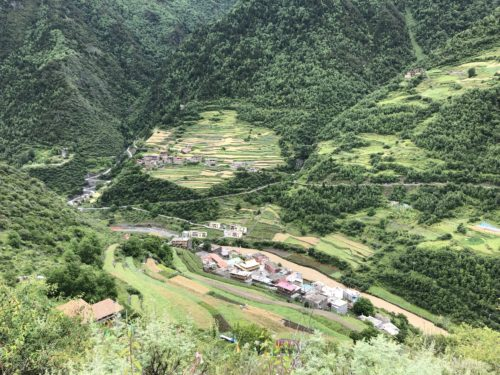
\includegraphics[width=5.20833in,height=3.90625in]{images/IMG_7199-500x375.jpg}
\caption{The Siyuewu village}
\end{figure}

The Siyuewu village

We are both botany laymen, so we collaborated with botanists from Yunnan
University of Traditional Chinese Medicine, in order to accomplish our
goal.

We went into the mountains together and learn from one another. The
field work is generally accompanied by one or several native speaker(s),
who identify plants and tell us about them: the name in the local
language, the morphology, and the uses.

\leavevmode\hypertarget{attachment_2139}{}%
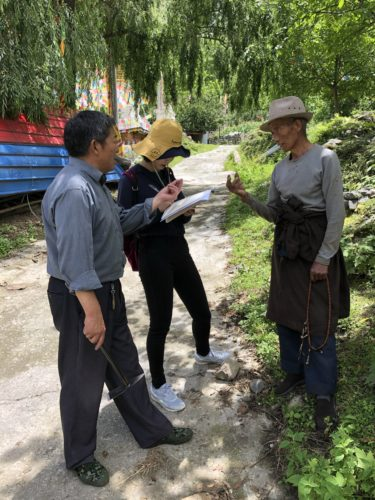
\includegraphics[width=3.90625in,height=5.20833in]{images/IMG_2558-375x500.jpg}

Shuya taking notes from native speakers

\leavevmode\hypertarget{attachment_2131}{}%

\includegraphics[width=5.20833in,height=3.90625in]{images/IMG_7418-500x375.jpg}

bsang gsol (bsang offering)

The botanists help us collect specimens, and teach us how to conserve
them. Normally, it is best to have flowers or fruits on the specimens,
so the botanists can make accurate identifications. But not everyone of
them happens to bloom or bear fruit within a given period of a year, and
that means we need field trips in different seasons. Summer is good
enough, anyway, as you can see most of the flowers and the weather is
pleasant.

\leavevmode\hypertarget{attachment_2135}{}%
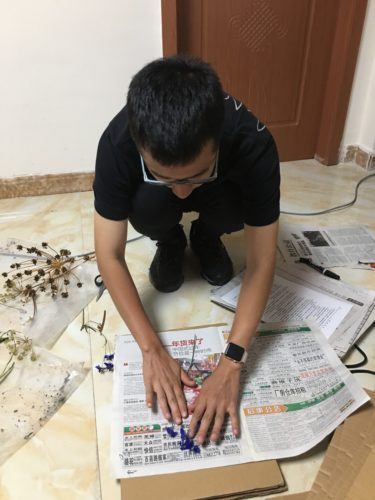
\includegraphics[width=3.90625in,height=5.20833in]{images/IMG_7423-e1575732106557-375x500.jpg}

Me making specimens

\leavevmode\hypertarget{attachment_2147}{}%
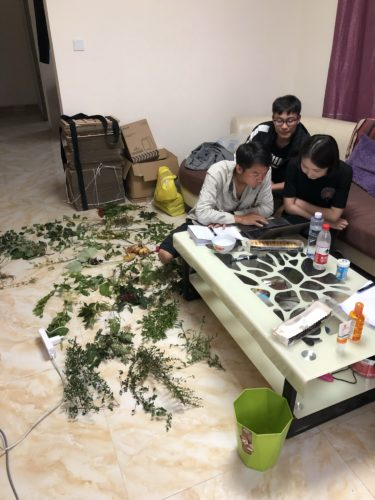
\includegraphics[width=3.90625in,height=5.20833in]{images/IMG_9705-375x500.jpg}

Shuya learning from the botanists

The specimens were then brought back to Yunnan, where the botanists are
based. They may have some secret weapon to help identify the species and
report us back with the scientific names. And us, the linguists, stayed
in the Rgyalrongic speaking regions to do our job: recording and
transcribing. Several native consultants are needed, as they might make
mistakes with the plant terms.

Some terms are quite funny. The burdock ( \emph{Arctium lappa L.} ), is
called \emph{pəɟə-rtsôs} in Brag-bar Situ. Literally, \emph{pəɟə̄} means
\enquote{mouse} and \emph{rtsôs} means \enquote{to touch}, so the term
globally means \enquote{touch by the mouse}.

\leavevmode\hypertarget{attachment_2159}{}%
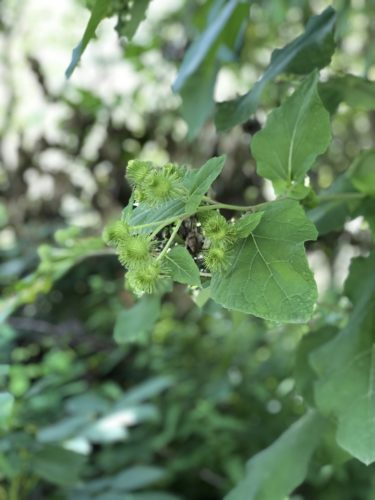
\includegraphics[width=3.90625in,height=5.20833in]{images/IMG_7164-e1575732684598-375x500.jpg}

Burdock

The Khroskyabs term \emph{mɑ̂venono} , literally meaning
\enquote{grandmother's breasts}, designates the flower of Salvia
przewalskii Maxim, as the purple flowers, accordingly, look like female
breasts with ptosis as they age.

\leavevmode\hypertarget{attachment_2167}{}%
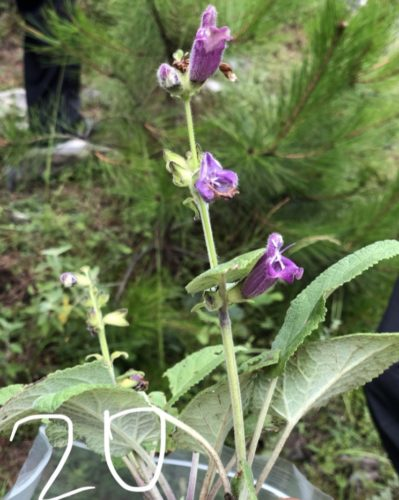
\includegraphics[width=4.15625in,height=5.20833in]{images/2711575733084_.pic_hd-399x500.jpg}

Salvia przewalskii Maxim

So, what could we do with linguistic ethnobotany? There could be many
benefits, both synchronically and diachronically, linguistically and
non-linguistically.

By comparing cognates between plant terms, we may get a better idea
about the sound correspondences across different Rgyalrongic languages
and improve our understanding of Rgyalrongic historical linguistics.
That some of the terms can be reconstructed into the proto-language
implies that the ancestors of all Rgyalrongic people already knew and
probably made use of those plants. Terms borrowed from other languages
can be sorted by layers, according to different stages of sound change.
We know that sound correspondences are always messy in Sino-Tibetan
languages, but plant term comparisons may tidy up the mess, and we can
also implement automatic methods (see for example {[}this post{]}) So it
is not impossible to know the relative chronology of plants known by
native speakers. Inference of the Proto-Rgyalrongic life could well be
made based on historical linguistic analyses (of course, we need more
cognates!). The table below shows the cognates found in the field work
this year.

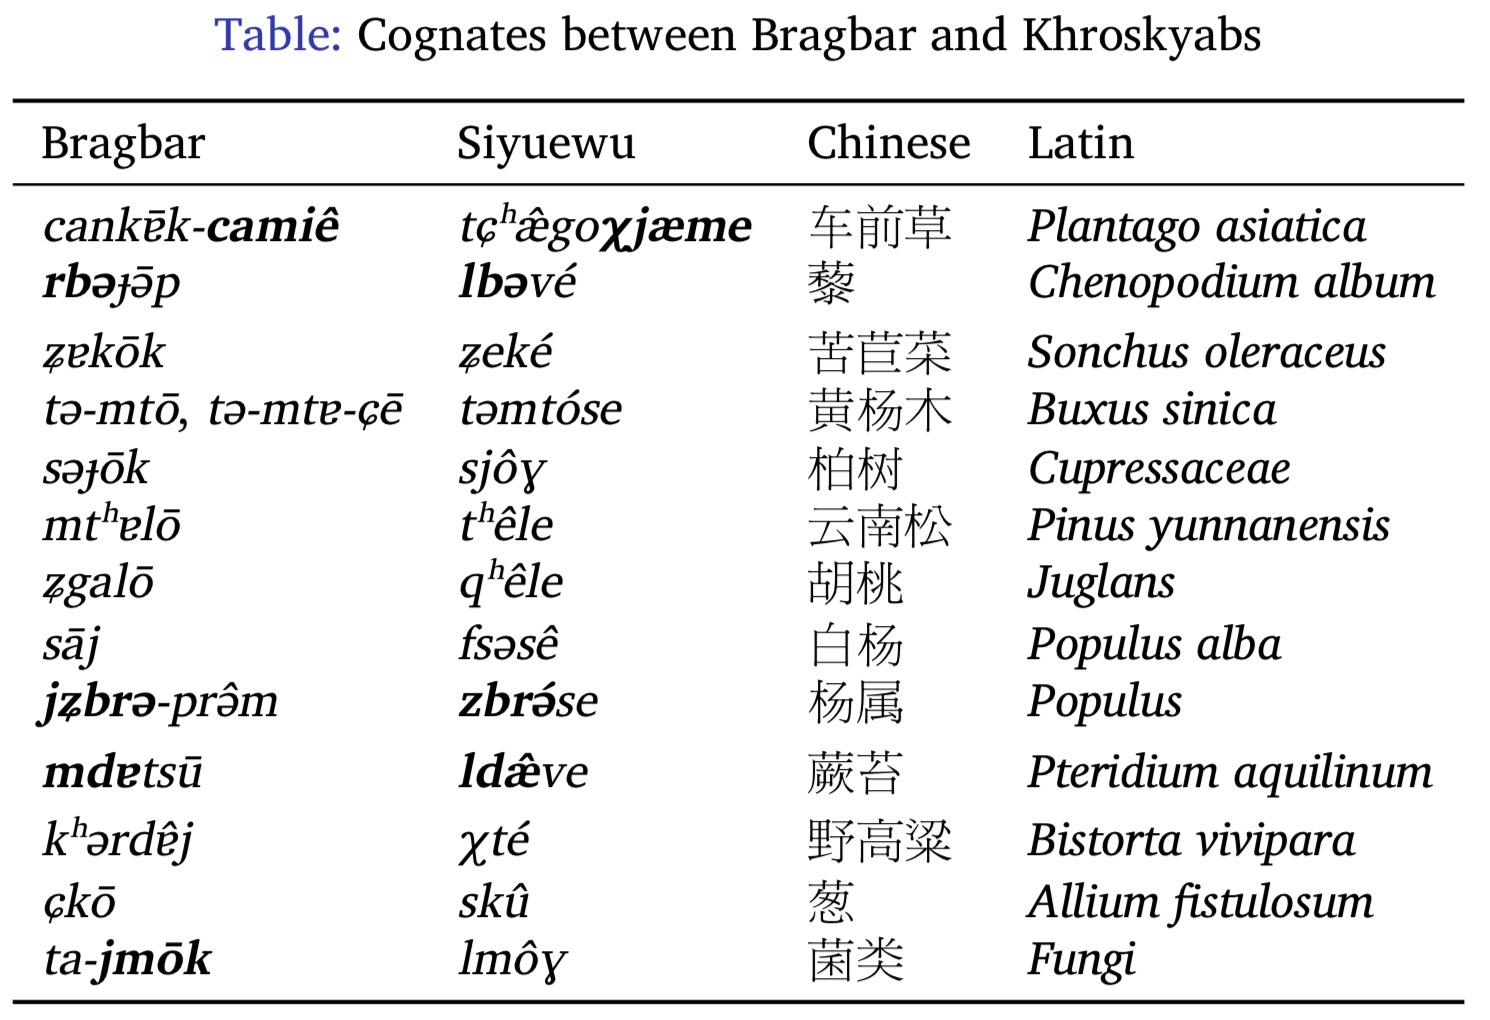
\includegraphics[width=5.29167in,height=3.625in]{images/2691575731829_.pic_hd.jpg}

Plant terms are a key to synchronic analyses of nominal constructions in
the modern languages. They cover nearly all kinds of nominal morphology,
commonly or rarely found in other nominals. From unanalysable terms, to
various types of compounding. Shuya and I gave a talk on this subject in
Tianjin this year (Lai and Zhang 2019). I am also looking forward to use
the method of word formation handling, when I have enough material,
developed by Nathanael, with his excellent paper accepted, Schweikhard
and List (forthcoming). The table below shows the cases of Tatpuruṣa in
Siyuewu Khroskyabs.

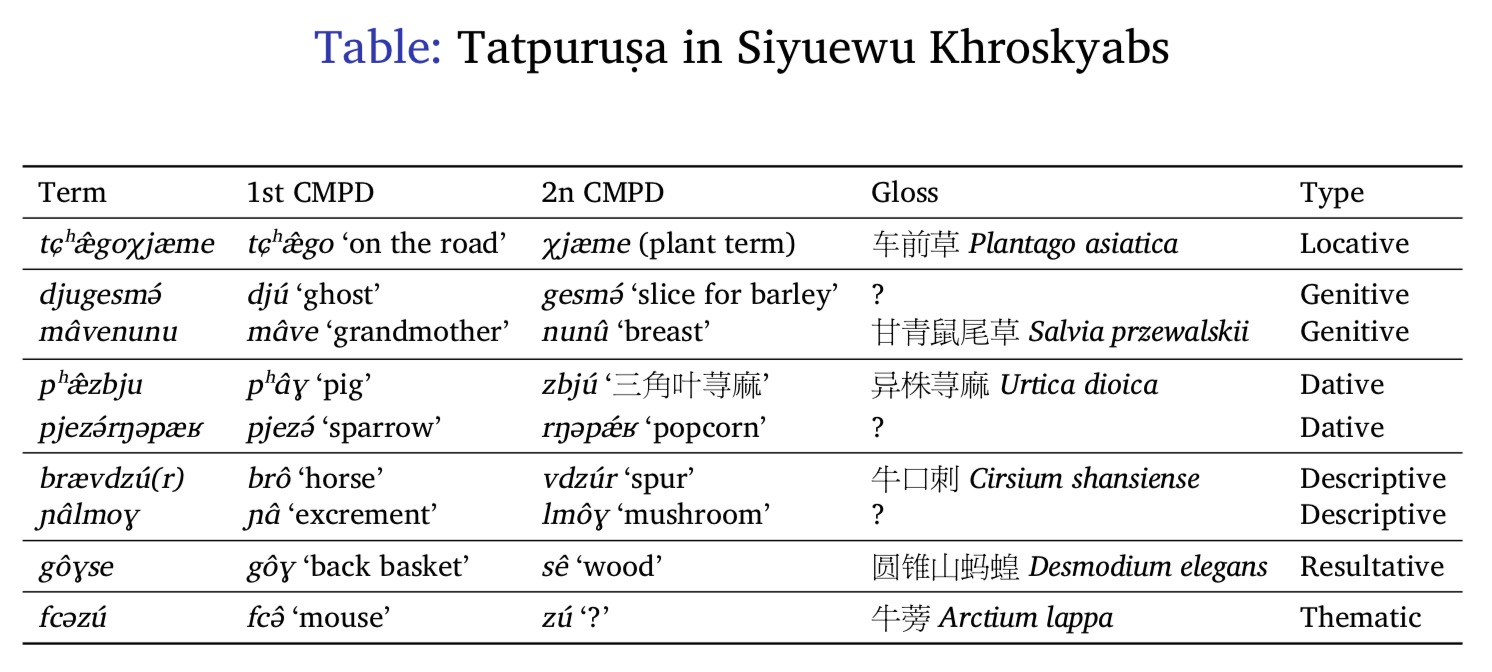
\includegraphics[width=6.11458in,height=2.75in]{images/2701575731864_.pic_hd.jpg}

The fruits produced from this project are not only to feed us, the
researchers, but also to be given back to the native speakers and the
entire society. We plan to publish an encyclopedia of local plants with
names, descriptions and sound files in Rgyalrongic languages (Hopefully
three languages, including Guillaume Jacques' Japhug).

\subsection*{References}

\nopagebreak\hangindent=0.7cm {\small Lounsbury, Floyd G. 1956.~A Semantic Analysis of the Pawnee Kinship
Usage. Language 32 (1): 158-194.}

\nopagebreak\hangindent=0.7cm {\small Hoijer, Harry. 1956. \enquote{Athapaskan kinship systems}. American
Anthropologist. 58 (2): 309--333. }

\nopagebreak\hangindent=0.7cm {\small Jacques, Guillaume. 2012d. The Tangut kinship system in Qiangic
per-spective. In Nathan W. Hill (ed.),~Medieval Tibeto-Burman Languages
IV, 211--258. Leiden: Brill. }

\nopagebreak\hangindent=0.7cm {\small Hsieh, Feng-fan. 1999. Theoretical Aspects of Zhuokeji rGyalrong
Phonology. National Tsing Hua University, Taiwan MA thesis. }

\nopagebreak\hangindent=0.7cm {\small Lai, Yunfan and Zhang Shuya. 2019. Plant terms as key to nominal
morphology in Rgyalrongic languages. Paper presented at the he Fourth
Workshop on Sino-Tibetan Languages of Southwest China. August 2019. }

\nopagebreak\hangindent=0.7cm {\small Schweikhard, Nathanael and Johann-Mattis List. under review.
Handling word formation in comparative linguistics. }

\nopagebreak\hangindent=0.7cm {\small  Zhang, Shuya. forthcoming. Brag-bar kinship system in synchronic and
diachronic perspectives. Bulletin of the School of Oriental and African
Studies. }

\vskip 2em
\framebox{\tabular{p{0.95\textwidth}}\textbf{Cite this article as}:
Yunfan Lai,
\enquote{Linguists love plants,
too!,}
in \emph{Computer-Assisted Language Comparison in Practice},
11/12/2019, \url{https://calc.hypotheses.org/2119}.\endtabular}


\end{document}
